% Fractal Intelligence: Conceptual Decomposition

\documentclass[11pt]{article}
\usepackage{emergentwisdom-longform}
\usepackage{xcolor}
\usepackage{hyperref}
\hypersetup{
  hidelinks,
  pdftitle={Fractal Intelligence: Conceptual Decomposition as Problem-Solving Infrastructure},
  pdfauthor={Henrik Westerberg},
  pdfsubject={A theory and architecture for cumulative intelligence through conceptual decomposition},
  pdfkeywords={fractal intelligence, conceptual decomposition, multi-agent systems, cognitive architecture, Solver contracts}
}
\usepackage{booktabs}
\usepackage{array}
\usepackage{float}
\usepackage{enumitem}
\usepackage{tcolorbox}
\tcbuselibrary{skins,breakable}
\usepackage{graphicx}

\usepackage{tikz}
\usepackage{pgfplots}
\pgfplotsset{compat=1.18}
\usetikzlibrary{positioning, shapes, shapes.geometric, arrows.meta, calc, shadows}

% Shared style for the concept-decomposition tree figures (\S\ref{sec:algorithm}).
\tikzset{concepttree/.style={
    concept/.style={rectangle, draw=black!70, thick, rounded corners=3pt, minimum height=0.55cm, align=center, fill=white, drop shadow, font=\scriptsize},
    leaf/.style={rectangle, draw=black!40, rounded corners=2pt, minimum height=0.45cm, align=center, fill=gray!5, font=\scriptsize\itshape},
    edge from parent/.style={thick, -Latex, black!50, draw},
    level 1/.style={sibling distance=4.2cm, level distance=1.4cm},
    level 2/.style={sibling distance=1.8cm, level distance=1.3cm},
}}

\definecolor{nodegray}{HTML}{5A5A6E}
\definecolor{diamondgray}{HTML}{4A4A5E}
\definecolor{accentblue}{HTML}{2979FF}
\definecolor{textwhite}{HTML}{EEEEF0}
\definecolor{labelgray}{HTML}{AAAABC}

\let\oldtexttt\texttt
\renewcommand{\texttt}[1]{\oldtexttt{\small #1}}

\newtcolorbox{rfbox}[1][]{colback=gray!5, colframe=gray!50, fonttitle=\bfseries\small, #1}

\ewlongtitle{Fractal Intelligence}{Conceptual Decomposition as Problem-Solving Infrastructure}
\author{Henrik Westerberg\\
\small{henrik.westerberg@emergentwisdom.org}}
\ewreviseddates{April 7, 2026}{September 10, 2026}

\begin{document}

\maketitle

\begin{abstract}
\noindent Human problem decompositions often inherit path-dependent conventions. Fractal Intelligence asks what a capability is made of, rather than which steps a familiar procedure follows. Reconsidering that structure may reveal inherited assumptions and overlooked concepts and mechanisms. The proposal organizes cumulative intelligence through bounded, concept-defined units that recursively decompose and reframe problems, compose higher-level capabilities, and preserve evaluated structures for reuse and revision across domains and scales.

A root Solver bounds the problem space. The search starts from a specific capability and moves through adjacent, broader parent concepts toward that root. At each step it records the parent kind (genus) and the child's distinguishing features (differentia), and examines sibling alternatives. It then retraces the route before decomposing the capability into contributions tested for necessity, independence, universality, and completeness. Specialization locates kinds; composition identifies what must work together. The Solver Contract gives individual and composite Solvers the same interface. Parent synthesis explains how child work is routed, combined, and checked as one outward capability. Models, humans, programs, or subtrees can perform the internal work, and one Solver may serve several parents without changing its contract. Expected gain relative to cost governs depth; content-addressed Pathway Memory retains evaluated routes to guide reuse and revision. Typed rejection can request a different decomposition; recurring validated structures may become shared reasoning routes. This organization can be distributed across systems, implemented by a single model, or practiced by a person.

Problem-solving benefits remain untested. Tests must assess whether fresh conceptual decompositions outperform equally persistent conventional approaches under matched compute and memory, whether independent decompositions recover recurring structure or useful complementary alternatives beyond arbitrary divergence, and whether reuse improves later problem solving.
\end{abstract}
\keywords{Fractal Intelligence, Conceptual Decomposition, Multi-Agent Systems, Cognitive Architecture, Solver Contracts}

\ewfrontmatterend

%==============================================================================
\section{Introduction}
%==============================================================================

This paper begins with two simple claims. First, solved reasoning should not evaporate. Consider a task-local agent system that discards the structure that produced an answer, or preserves only a transcript that later systems must interpret from scratch. An evaluated solution graph---its concepts, route, outputs, gate results, provenance, and outcome---should remain globally addressable, subject to permissions, so the next relevant problem can begin from what has already been worked out.

Second, the inherited way of cutting problems may not be the best one. A role-based multi-agent workflow can reproduce the task boundaries of human organizations: assess, plan, assign, execute. Those boundaries coordinate people well, but they are path-dependent products of institutions and history. A model trained on human text does not escape them by itself; it inherits the categories as well as the knowledge.

The useful thought experiment is an alien analyst arriving with no business school, ministry, or professional guild to imitate. Asked to understand an economy, it does not begin from our departments or procedures. It asks what an economy is actually made of, moves upward through adjacent abstractions, tests each proposed parent against its siblings, then retraces that route and carves downward from the resulting frame. The thought experiment places an explicit decomposition discipline between inherited convention and the solution while recognizing that any language model remains culturally conditioned.

The four tests developed here---necessity, independence, universality, and completeness---bring together MECE-style partitioning and the Aristotelian search for properties that define every member of a category. They provide one practical discipline, not the only possible method, and do not guarantee a uniquely correct tree. A fresh carve may reveal structure convention missed, or it may re-derive the conventional answer and make its hidden reasoning explicit. The imperative to look is therefore distinct from the empirical claim that looking wins; the latter must be established against equally resourced conventional baselines.

The broader research program distinguishes three complementary motions: \emph{jump farther} by changing the causal premises from which mechanisms are derived, \emph{search wider} by mapping a candidate population and directing generation toward underrepresented mechanism families, and \emph{decompose deeper} by recursively isolating the concepts on which a problem depends. Orthogonal Insight studies one long-range displacement operator~\cite{westerberg2025strangeworlds}; the companion Ontology work studies population-level search state~\cite{westerberg2026ontology}; this paper asks how selective depth, typed composition, and cross-problem persistence can become cumulative intelligence. The studies emphasize different operations and retain different principal objects: a candidate ontology maps proposed interventions, a Solver graph routes concept-defined capabilities, and an evaluated solution graph records what was attempted and checked so useful structure can persist. No experiment has evaluated all three motions together.

Recursive encapsulation is core to this realization: bounded representations and interfaces make lower-level complexity usable at a higher level of cognitive organization. Major evolutionary transitions provide a precedent in which lower-level entities became integrated into higher-level individuals able to function as units at another scale~\cite{west2015transitions,michod2007individuality}. The Solver architecture reverses the order of boundary assignment for engineering: a root Solver encapsulates the complete problem space of its deployment before particular problems are decomposed within it. Section~\ref{sec:emergence} develops this evolutionary precedent and its limits.

There is reason to look. Human expertise is largely implicit: pattern matching, norms, and intuitions accumulated through practice. We rarely write down the \emph{invisible thinking}~\cite{westerberg2026entangled, westerberg2026understanding} that produces a conclusion, and we rarely sustain the deliberate, dimension-by-dimension reasoning Kahneman calls System~2~\cite{kahneman2011}. Machines can sustain it, but only if given structure in which to do so. Instead of asking ``how would a human solve this?'', the architecture asks: ``what is this problem made of?''

Consider creating a restaurant. The conventional approach is a sequence of tasks: research the market, secure funding, find a location, hire a chef, design a menu, build out the space, obtain permits, launch marketing, open. This familiar sequence is useful for coordinating execution, but it describes activities rather than reusable conceptual structure.

A conceptual decomposition instead asks two different questions. First: what does it mean to \emph{create} something? This decomposes into intent, form, realization, fit, and viability---dimensions that apply to creating anything, whether a restaurant, a curriculum, or a building. Second: what \emph{is} a restaurant? This decomposes into nourishment, experience, flow, economics, and identity---candidate differentiated dimensions of the thing itself. Each dimension corresponds to a distinct failure mode: nourishment concerns the primary offering, experience the form of service, and flow the coordination of people and resources. For example, designing a menu gives form to the restaurant's nourishment; checking whether that menu can sustain the business brings viability and economics into the same task. Tasks emerge at the intersection of these two decompositions, but the conceptual structure is what can persist and transfer.

The distinction is relational rather than grammatical. A task decomposition partitions a chosen route to an outcome into actions, stages, or roles. A conceptual decomposition partitions the capability or problem class itself into functions, constraints, or causal dimensions claimed to be constitutive of a qualifying realization. The same word can occur in either: an action may itself become the subject of conceptual decomposition when treated as a capability, while every concept-defined Solver receives concrete Tasks when invoked. Abstract names and persistence alone do not establish the distinction; what matters is whether the children describe a procedure for producing one result or the proposed structure through which many possible procedures and instances can route.

Once decomposed, each dimension can be assigned to a solver isolated behind its own boundary. Flow---how people and resources move through space and time---shares recurring concerns across a restaurant, a hospital, a transit system, and an irrigation network. Recurring dimensions may therefore become permanent infrastructure---reasoning highways---although the further claim that repeated use sharpens them remains untested.

If that wager pays, an AI assistant could consult something larger than itself: a persistent reasoning network, analogous to the internet's relation to any single computer. The network would decompose a submitted problem, solve parts in parallel, and reuse structures developed for earlier problems. The assistant would remain responsible for contextual judgment, weighing what returns and overruling it when necessary. Such a system would provide an internet for reasoning rather than retrieval: problems would be submitted for structured resolution rather than answered from model weights alone.

Human civilization already approximates this pattern: a hospital retains diagnostics, surgery, pharmacology, and rehabilitation as specialist structures through which successive patients route. Each case concludes; the hospital's specialist structures persist. The architecture proposed here makes such structures explicitly composable, content-addressed, and persistent at machine scale.

The remainder of the paper separates four evidential layers. Sections~\ref{sec:algorithm}--\ref{sec:contract} define the architectural core; Sections~\ref{sec:learning}--\ref{sec:substrate} develop proposed protocols, learning dynamics, and long-horizon implications; Section~\ref{sec:prototype} reports structural construction and implementation probes; and Sections~\ref{sec:related}--\ref{sec:limitations} distinguish related work, present evidence, and state the unresolved tests. The breadth of an implication is not evidence that its mechanism has been implemented.

\subsection{The Concept of Fractal Intelligence}
\label{sec:why-fractal}

\begin{quote}
\textbf{Fractal intelligence} \emph{is a form of cumulative intelligence in which bounded, concept-defined units recursively decompose and reframe problems, compose child work into higher-level capabilities, and preserve evaluated structures for reuse or revision across problems, domains, and scales.}
\end{quote}

Put compactly, fractal intelligence is problem solving through conceptual decomposition, with structure that persists and can be restructured. The Solver architecture developed here is one concrete realization of that broader category, using a root boundary, typed contracts, acceptance gates, Pathway Memory, and a marginal-value rule; these mechanisms do not exhaust the category.

The pattern is organizational rather than a claim about deployment scale. A conceptual hierarchy by itself is only a representation, not yet an intelligent problem-solving process. For one active root Task, specialization nodes locate and frame the problem, while each invoked compositional node supplies a bounded contribution to its parent; parent synthesis recursively carries those differentiated contributions toward the root result. Nodes outside the active solution graph need not run. The resulting organization may be distributed across many humans, models, and programs, or one person or model may enact a persistent repertoire of Solver roles internally. In the latter reading, an internal Solver network is an explicit scaffold or functional description of problem solving, not a claim that human cognition literally contains typed Solver Contracts. Because the structure persists, outcome evidence may revise routing, sharpen or replace capabilities, and split, merge, or reparent nodes as described in Section~\ref{sec:learning}. Persistence makes cumulative improvement possible; it does not guarantee it.

In this realization, a composite parent coordinates child work behind one contract boundary, so its subtree presents one Solver interface to the caller. A deployment may use one model or many. Because routing is organized by declared conceptual contracts rather than one fixed domain workflow, the architecture is intended to accept problems from many domains; whether its coverage becomes genuinely general is an empirical question. From the outside, it aims to behave as a single general-purpose problem solver. From the inside, it is specialists all the way down.

The foundation of this realization is first-principles thinking. When a node is decomposed, it asks the same question: what are the irreducible dimensions of this concept relative to its current outward promise and intended range of instances? The term \emph{fractal} is used in an organizational rather than strictly geometric sense: the same relationship recurs at multiple scales. A problem can be decomposed into conceptual subproblems; each subproblem can be decomposed again; and a solved substructure can itself function as a component of a larger one. The five-surface Solver Contract expresses this recurrence uniformly at every level. The resolution increases; the organizational pattern remains.

No individual node needs to be generally intelligent: the intended capability comes from composing specialists through the contract. Typed invocation boundaries can keep the generator's and verifier's working contexts distinct even when both are bound by the same public \texttt{AcceptSpec}; the generator need not receive the verifier's private deliberation or verdict. Section~\ref{sec:synergy} develops this isolation claim and its evidence.

Candidate nodes arise in two ways. Specialization membranes are bounded nodes that locate kinds along the upward abstraction route; compositional Solvers are generated by the downward four-test search operator developed in \S\ref{sec:algorithm}. Evaluated solution graphs enter the archive; recurrent, validated, or uniquely useful subgraphs may be promoted into the active serving layer---the structures selected for routine use. Pathway Memory (\S\ref{sec:partition}) records experience with routes and their quality, depth, and cost, informing later routing under the marginal-value rule (\S\ref{sec:mvr}). The architecture permits alternative search operators, catalogues, and routing policies. The ten protocols are worked examples whose value does not require convergence on a definitive ontology.

\subsection{Theses}
\label{sec:theses}

Seven theses elaborate the two commitments above: retain solved structure, and search for leverage in how problems are decomposed. They do not have the same evidential status; some are architectural claims, others scaling or governance implications. Each is paired with a failure condition. The decisive empirical program has three parts: whether conceptual decomposition beats equally persistent conventional solving at matched compute, whether independently derived carves reveal recurring invariants or complementary utility beyond chance, and whether reuse improves subsequent problem solving. Together, these tests separate architectural feasibility from claims of superior performance, cross-carve invariance, and cumulative benefit.

\emph{Thesis 1: Solved structure should persist, and conceptual structure is the candidate unit of transfer} (\S\ref{sec:algorithm}, \S\ref{sec:topology}, \S\ref{sec:genreduce}--\S\ref{sec:meta-protocols}). An evaluated solution graph should remain available rather than dissolve after execution. Because task plans can also be cached, memory alone does not establish the distinctive thesis: the empirical bet is that conceptual decomposition---what a problem \emph{is made of}, not merely what to do next---produces units that transfer farther across domains than equally persistent task traces. The protocols instantiate candidate units of transfer, while the construction artifact's prompt-conditioned, structurally recorded reuse (\S\ref{sec:prototype}) does not establish superiority. \emph{Falsification:} give concept-decomposed and task-decomposed systems equal global memory, compute, and outcome feedback. If task traces match conceptual graphs in cross-domain reuse and solution quality without implicitly reconstructing concepts, conceptual structure is not a superior transfer unit; the separate value of persistence would remain unresolved.

\emph{Thesis 2: Additional intelligence is found by zooming deeper into the fractal, up to the point where incremental decomposition cost exceeds incremental cognitive gain} (\S\ref{sec:selective-depth}, \S\ref{sec:mvr}, \S\ref{sec:jumps}). Deeper conceptual decomposition can sharpen an analysis by isolating sub-concepts that a shallow treatment blends together. Where a ground truth exists, this may improve accuracy; for normatively contested concepts, it instead yields a more fully mapped disagreement structure. The marginal-value rule bounds the claim. \emph{Scope-limiting result:} if well-tuned uniform-depth or shallower solvers systematically outperform marginal-value-guided deeper decomposition across a problem class, then depth is not a general source of intelligence for that class and the rule must be reformulated.

\emph{Thesis 3: Organizing structure can contribute intelligence beyond the components alone} (\S\ref{sec:contract} and \S\ref{sec:substrate}). Component capability still constrains the whole, but a parent's Tasks, routing, synthesis, and gates coordinate child work and make gate outcomes locally assignable without a shared loss function. \emph{Falsification:} if untyped, loose coordination among the same components, under matched compute and task distribution, produces equivalent compositional gains and equivalent per-node learning, the structure-contributes-intelligence thesis is false.

\emph{Thesis 4: Cognitive isolation enables productive extremes} (\S\ref{sec:synergy}). Competing objectives can compromise one another when they share a forward pass or weights, as the Safety Tax illustrates~\cite{Huang2025}. Contract-bounded Solvers instead separate cognitive modes so generation and verification need not soften toward one another. \emph{Falsification:} if a single monolithic model, trained with equivalent compute and without hidden modular isolation, matches the composition's capability on tasks requiring genuinely competing modes, the productive-extremes thesis is false.

\emph{Thesis 5: Typed rejection turns failure into a structural reframing signal} (\S\ref{sec:seams} and \S\ref{sec:synergy}). A rejection can name a failed structural relation and ask the upstream Solver to change its frame rather than merely produce another answer. The companion study documents an analogous precursor: curator rejection with mechanism-level redirection, followed by a retry that changed the causal relation~\cite{westerberg2026ontology}. It did not isolate that effect or include a matched monolithic baseline. \emph{Falsification:} if an equally resourced retry protocol receiving the same history and pass--fail outcome, but no typed structural diagnosis, matches both the frequency and utility of relation-changing reframes and the resulting outcomes, the stronger reframing-over-retry claim fails.

\emph{Thesis 6: Evaluation is itself a Solver, and the apparent regress terminates} (\S\ref{sec:seams} and \S\ref{sec:meta-protocols}). If gates do cognitive work, evaluation is a cognitive task and every evaluator needs its own evaluator. The Solver Contract terminates this regress at two ends: mechanically decidable checks at the bottom (schema checks, hash matches, test vectors), whose verdicts require no language-model judgment even though their specifications and implementations can still be wrong; and the proposed \texttt{OutcomeArbiterSolver} at the top, grounded in human judgment on open-ended problems and in objective checks on verifiable ones. Evaluation therefore terminates in either mechanically decidable criteria or explicitly identified human judgment. \emph{Failure condition:} if evaluator Solvers cannot be grounded more reliably than monolithic evaluators on matched open-ended and verifiable tasks, then this termination strategy is not an advantage over simpler evaluation architectures. The philosophical grounding of normative judgment at the top remains an open problem regardless of this architecture's choice.

\emph{Thesis 7: A machine-scale realization of fractal intelligence could become a social-organizing principle} (\S\ref{sec:global}). Machine-speed coordination through typed contracts, content-addressed patterns, and persistent reasoning may admit organizational structures not derived from the constraints of biological minds. The promise is compositional intelligence at unprecedented scale; the risk is replacing slow, legible, contestable structures with fast, opaque, optimized ones~\cite{westerberg2026entangled}. \emph{Scope-limiting result:} if large-scale typed-contract coordination offers no capability, efficiency, or reliability beyond biological coordination and conventional software organizations on matched tasks, the claim reduces to an engineering pattern. Whether such coordination would improve or erode institutional legitimacy is an independent normative question.

\subsection{What This Architecture Adds}
\label{sec:adds}

The theses above are claims about what the architecture may produce. This subsection specifies six concrete mechanisms proposed to produce them---the architectural primitives on which the theses rest. Some are exercised by the mandatory-abstraction construction and experimental reference implementation described in Section~\ref{sec:prototype}, while others remain design commitments. The theses define the tests; the mechanisms define the proposed implementation.

\emph{Self-similar contracts.} Every node, whether orchestrator, specialist, or leaf, presents the five-surface Solver Contract (Section~\ref{sec:contract}), with Manifest and Execute mandatory and the other three surfaces optional and discoverable. A leaf and a compatible thousand-node subtree can therefore present the same contract boundary to the caller. Because the boundary is uniform, a compatible subtree that solved a problem at depth~7 can be imported at depth~2; without this recursive closure, the other mechanisms lose their foundation.

\emph{Gates that request conceptual restructuring.} A structural rejection is a typed diagnostic naming the failed relation and asking the upstream Solver to change its approach rather than merely rephrase it. The retirement-system traces in Section~\ref{sec:synergy} illustrate an analogous redirection path; they do not implement a Solver Contract gate or isolate the controller's causal effect from the companion system's other differences.

\emph{Cognitive isolation enabling productive extremes.} Cognitive mode is declared in the Manifest and separated by typed invocation boundaries, so each mode can operate without direct access to the others' invocation context (Thesis~4)~\cite{Huang2025}.

\emph{Economic depth governance.} The marginal-value rule (Section~\ref{sec:mvr}) decides at every node whether the expected gain from further decomposition justifies its incremental cost.

\emph{Persistent decomposition and learning through reuse.} The decomposition crystallizes as a content-addressed pattern importable by hash (Section~\ref{sec:sema}): what persists in that reusable specification is the anatomy of a competence, not an answer. The evaluated solution graph also retains outputs and their evaluation history. The routing layer can direct structurally similar problems to a common Solver through the uniform contract, accumulating cross-domain signal to guide later refinement and the formation of validated reasoning highways (Section~\ref{sec:reuse-measurement}).

\emph{Revisable typed topology.} In the proposed architecture, reviewed evidence can insert a higher parent, retire a shortcut, split a Solver doing two conceptual jobs, or merge duplicate boundaries. Specialization and composition edges retain different meanings, while immutable patches preserve what changed. The construction artifact demonstrates graph construction and higher-parent insertion, not autonomous feedback-driven topology learning; its behavior is reported in Section~\ref{sec:prototype-results}.

\begin{table}[H]
\centering
\small
\caption{Illustrative role-based task pipeline vs.\ the proposed Solver Tree. The pipeline column describes the task-local comparison used here; task workflows can also preserve reusable traces. Reused constituent trees can form a multi-parent graph.}
\begin{tabular}{@{}lp{5cm}p{5.5cm}@{}}
\toprule
& \textbf{Role-Based Task Pipeline} & \textbf{Solver Tree} \\
\midrule
Organizing principle & Actions, stages, or roles in a chosen route & Constitutive capability or dimension (tasks route through it) \\
Identity basis & Assigned role in the workflow (the ``who'') & Concept/Interface (the ``what'') \\
Topology & Usually specified around a workflow & May adapt through observed use \\
Boundaries & Often natural-language handoffs & Typed, gated (reject + diagnosis) \\
Depth allocation & Often stage-based & Selective (marginal-value rule) \\
Failure signal & Often reported at task level & Checked at seams; detected failures may request reframe \\
Cognitive mode & Usually attached to task roles & Declared; separated by typed invocation \\
Output & An answer and any retained task trace & An answer + evaluated conceptual structure \\
Persistence & Often task-local or trace-based & Evaluated structure retained; recurrent patterns addressable \\
\bottomrule
\end{tabular}
\label{tab:pipeline-vs-solver}
\end{table}

\subsection{Contributions}
\label{sec:contributions}

This paper's central contribution is the claim that conceptual decomposition can become cumulative reasoning infrastructure: problems are located through mandatory upward abstraction, decomposed recursively downward into concept-defined Solvers, selectively deepened under a marginal-value rule, and retained as revisable evaluated structures that later problems can reuse. Its components have ancestors in means--ends analysis, division of cognitive labor, hierarchical and modular decomposition, distributed cognition, and cybernetic regulation~\cite{newell1972,babbage1832,simon1962,minsky1986,parnas1972,ashby1956}; self-similar organization~\cite{hewitt1973actor,Warnecke1993,Ryu2003}; contract coordination~\cite{Smith1980,khattab2024dspy,zhuge2024gptswarm,YeTan2026agentcontracts}; morphological analysis~\cite{zwicky1969}; and persistent workflow reuse~\cite{singh2025graphmemoized}. What is distinctive is the proposed combination of mandatory upward abstraction, recursive downward decomposition, contract-bounded composition, structural reframing, and accumulated reuse. Section~\ref{sec:related} develops the comparisons.

The four tests, and the universality test in particular, are intended to produce candidates whose relevance survives changes in concrete task and domain: they search for axes that recur across the range of instances currently claimed for the parent capability. That range is provisional and may widen, narrow, or be reframed. Independent carves may therefore recover common sub-concepts, but convergence is a prediction rather than a guarantee and is not the only possible success. The empirical test must measure both recurring invariants and whether divergent carves add utility beyond arbitrary divergence. In the mandatory-abstraction construction, reuse occurs inside one theory-conditioned graph; it demonstrates structurally accepted routing and higher-parent insertion, not independent discovery or highway formation.

Within the proposed Solver architecture, two complementary frameworks operationalize one route toward that idea: the \textbf{Theory of Depth} (Section~\ref{sec:ri}) governs when and where to decompose, while the \textbf{Solver Contract} (Section~\ref{sec:contract}) specifies how concept-defined Solvers compose through typed surfaces and gates. Orthogonal Insight and ontology-governed expansion are related search methods in the broader program, compatible with this architecture but neither definitions of fractal intelligence nor empirical results of the mandatory-abstraction construction reported here. Consequences of the proposed substrate include productive extremes (Section~\ref{sec:synergy}), localized learning (Section~\ref{sec:learning}), and a possible cognitive commons (Section~\ref{sec:global}).

The contributions occupy different evidential levels: the \emph{formalization} is specified and partly instantiated; the \emph{protocols} are design proposals; and the \emph{unifying claim} that conceptual decomposition enables cross-domain reuse remains an empirical hypothesis for the reproduction study in Section~\ref{sec:limitations}.

%==============================================================================
\section{The Conceptual Decomposition Algorithm}
\label{sec:algorithm}
%==============================================================================

This section makes one first-principles decomposition operator explicit enough to be executed by large language models. The four tests and pseudocode are a starting discipline rather than a complete specification of creative reasoning; practical implementations may use judgment, iteration, hybrid collaboration, or alternative search operators. Three author-designed examples illustrate the intended cross-domain candidates; machine-generated decompositions appear in the canonical mandatory-abstraction construction in Section~\ref{sec:prototype}. The architecture turns first-principles decomposition from an individual reasoning practice into an explicit, inspectable coordination procedure without assuming that this procedure exhausts the possible good carves.

\subsection{Concepts, Capabilities, Tasks, and Context}
\label{sec:concept-task}

A \emph{concept} is a candidate invariant used to organize the problem space: either a kind located through specialization or a constitutive dimension linked through composition. A \emph{capability} is the outward function through which that concept becomes operational. A \emph{Solver} is the contract boundary around an implementation of the capability, whereas a \emph{Task} is one invocation carrying particular inputs, constraints, budget, and acceptance criteria. \emph{Context} comprises the invocation-specific and parent-local conditions required to apply the capability without silently redefining its shared core. A parent's \emph{synthesis} states how its children's differentiated contributions, together with routing and integration, realize the outward capability promised at its own boundary.

The restaurant example above establishes the relational concept--task distinction. Here the further operational distinction is between reuse and transfer: selecting the same stored node or content-addressed Solver again is \emph{structural reuse}; claiming that competence transferred requires stronger evidence that its contract remained valid and its use improved or preserved relevant outcomes in the new context.

The four tests interrogate a \emph{provisional claim frame}: the outward capability being promised, the purpose for which it is being decomposed, and the range of instances over which the carve claims relevance. This frame makes ``necessary,'' ``universal,'' and ``complete'' claims interpretable; it does not fence in candidate generation. Upward abstraction, lateral reframing, or evidence from use may revise any part of the frame, and several incompatible frames or carves may coexist for comparison. The architecture records what each carve claims so that later routing and outcomes can test it. The carve is generative as well as organizational: changing it changes which dimensions receive dedicated reasoning and which mechanisms can be composed, potentially making previously unconsidered solution families locally generable. That possibility is a hypothesis to test, not a consequence of passing the four tests.

\subsection{Mandatory Abstraction Before Decomposition}
\label{sec:mandatory-abstraction}

The four tests answer what a concept is made of after the relevant concept has been located. They do not by themselves answer where a concrete stated problem belongs in a persistent graph. A complete construction pass therefore begins with the most specific reusable capability that frames the problem and follows conceptually adjacent \emph{specialization} relations upward until it reaches \texttt{RootSolver}. At every proposed attachment, the model searches existing and plausible siblings and records the parent genus, the child's differentia, how the higher frame changes the later carve, whether the contracts fit, and whether an informative intermediate parent has been omitted. A broad umbrella is not enough: an intermediate parent is warranted when it changes routing, exposes a reusable invariant, or changes the dimensions visible below.

The resulting ascent is then traversed in exact reverse order. After that traversal reaches the specific composite, the case applies the four-test procedure to ask what the capability is made of and binds the accepted dimensions through \emph{composition} edges. The relation types must not be conflated: specialization says that a child is a kind or realization of its parent and supplies an abstraction route; composition says that a child supplies a differentiated contribution required to realize its parent's outward capability. Specialization remains open-world---sibling search does not claim to enumerate every possible kind---whereas completeness is claimed only for the constitutive composition set. Higher abstraction is mandatory for locating a case; additional downward depth remains governed by the marginal-value rule.

\begin{figure}[!htb]
\begin{rfbox}
\small
\begin{verbatim}
LOCATE_AND_DECOMPOSE(problem, graph, depth_budget):
  subject <- identify_specific_capability(problem)
  ascent <- [subject]
  while last(ascent) != RootSolver:
    parent <- search_adjacent_parent(last(ascent), graph)
    siblings <- search_observed_and_plausible_siblings(parent, graph)
    if an informative intermediate changes routing or the later carve:
      parent <- insert_or_reuse_intermediate(parent, siblings)
    record genus, differentia, reframing effect, contract fit,
           omitted-parent search, and sibling search
    ascent.append(parent)
  route <- reverse(ascent)
  traverse(route)
  axes <- DECOMPOSE_CONCEPT(subject, depth_budget)
  synthesis <- explain_how(axes, realize=subject.outward_capability)
  return route, axes, synthesis
\end{verbatim}
\end{rfbox}
\caption{The complete construction motion. The ascent locates the problem in an abstraction hierarchy; the reverse traversal applies that frame before the downward four-test carve. The required record makes the proposed topology inspectable without claiming access to an oracle's private reasoning.}
\label{fig:locate-and-decompose}
\end{figure}

This procedure constrains the public topology artifact, not the model's hidden sequence of thought. The model remains responsible for semantic judgment; deterministic validation can check rootedness, edge types, exact route reversal, and artifact integrity, but not whether a parent is insightful or true.

\subsection{The Four-Test Search Operator}

When decomposing a concept, the operator does not ask ``what are the steps to accomplish this?'' (that produces a procedural carve). It asks: \emph{what differentiated dimensions must be addressed for this capability to function across the instances it currently claims?} The aim is a candidate low-coupling basis of the capability, not a proof of metaphysically final categories. Four questions generate and criticize candidate dimensions:

\emph{Necessity.} Relative to the outward capability currently being claimed, if you removed this sub-concept, would the parent still function? If removal causes the promise to collapse, the sub-concept is load-bearing. An economy without selection lacks a mechanism for determining what gets produced. Education without assessment lacks a systematic way to determine whether learning occurred.

\emph{Independence.} Can you change or reimplement one sub-concept without forcing the same revision in the others? You can redesign an economy's selection mechanism (from market to planned production) without changing your theory of fairness. You can redesign an educational assessment system without altering the content curriculum. Zero interaction is not required; the practical criterion is lower coupling, visible through counterfactual change propagation, routing overlap, and recurrent joint failures. If two candidates cannot vary or fail separately, merge them, move shared context to their parent, or search for a better cut.

\emph{Universality.} Does every instance in the range currently claimed for the parent capability contain this sub-concept? Candidate economic axes should recur across hunter-gatherer, feudal, capitalist, communist, and post-industrial systems; candidate educational axes should recur across Montessori schools, doctoral programs, and historical apprenticeships. A sub-concept limited to particular implementations, such as stock-market regulation or multiple-choice testing, is not universal over that range---but it may remain a valid specialization under a narrower claim.

\emph{Completeness.} For the current outward promise and analytic purpose, if you addressed all the sub-concepts, would you have a functioning instance of the parent capability? If something is missing, there is an axis, interaction, or framing assumption the carve has not represented.

The procedure combines two related but distinct disciplines. Necessity, independence, and completeness echo the Mutually Exclusive, Collectively Exhaustive principle formalized in Minto's Pyramid Principle~\cite{minto1985pyramid} and earlier decomposition methodology. Upward classification follows the Aristotelian genus-and-differentia form: name the more general kind shared with siblings, then state what distinguishes the selected child~\cite{aristotle_categories}. Downward decomposition uses all four tests; universality has a mathematical analogue in Formal Concept Analysis~\cite{wille1982fca}, where a formal concept's intent is the attributes shared by all objects in its extent. Genus and differentia do not make an observed sibling set complete: specialization is open-world, whereas completeness belongs to a claimed set of constitutive children. The contribution here is to package these disciplines as an LLM-executable construction procedure. Natural human concepts often exhibit graded, prototype-like structure rather than strict necessary-and-sufficient membership~\cite{rosch1978principles}; the tests are disciplines for assessing candidate reusable Solver boundaries, not a descriptive theory of human categorization, an oracle, or a proof of a uniquely correct ontology.

Then recurse: each sub-concept is itself a concept. Apply the same four tests. The recursion terminates when a sub-concept is concrete enough to be addressed directly by a single Solver---the point at which the marginal-value rule (Section~\ref{sec:mvr}) indicates that further decomposition would cost more than it yields.

\begin{figure}[!htb]
\centering
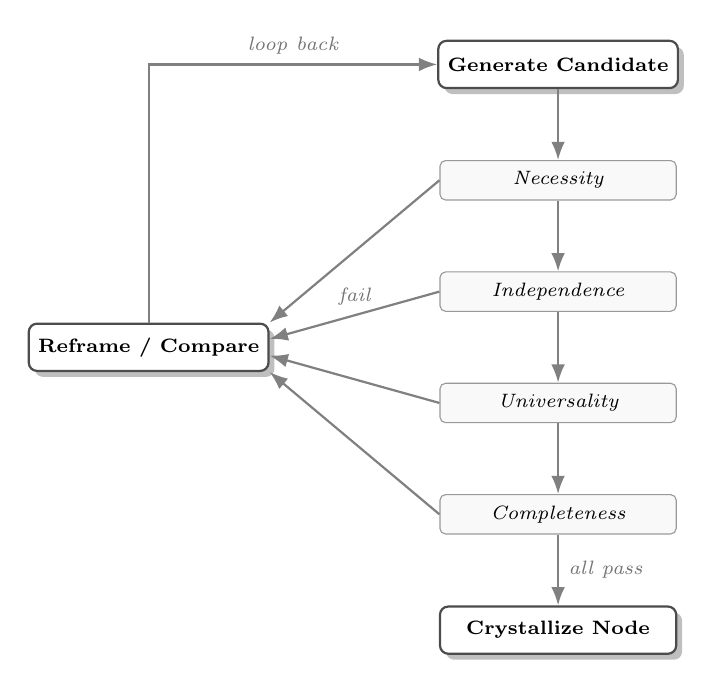
\begin{tikzpicture}[
    node distance=0.9cm,
    >={Latex[length=4pt]},
    proc/.style={
        rectangle, rounded corners=3pt,
        minimum width=3.0cm, minimum height=0.6cm,
        draw=black!70, thick, fill=white, drop shadow,
        align=center, font=\scriptsize\bfseries
    },
    test/.style={
        rectangle, rounded corners=2pt,
        minimum width=3.0cm, minimum height=0.5cm,
        draw=black!40, fill=gray!5,
        align=center, font=\scriptsize\itshape
    },
    arr/.style={thick, -Latex, black!50},
    lbl/.style={font=\scriptsize\itshape, text=black!55},
]

% Main column
\node[proc] (gen) {Generate Candidate};
\node[test, below=of gen] (nec) {Necessity};
\node[test, below=of nec] (ind) {Independence};
\node[test, below=of ind] (uni) {Universality};
\node[test, below=of uni] (comp) {Completeness};
\node[proc, below=of comp] (crys) {Crystallize Node};

% Reframe positioned at the vertical center of the tests, shifted left
\node[proc] at ($(ind)!0.5!(uni) + (-5.2, 0)$) (ref) {Reframe / Compare};

% Main pass flow (straight column, single "pass" label at the end)
\draw[arr] (gen)  -- (nec);
\draw[arr] (nec)  -- (ind);
\draw[arr] (ind)  -- (uni);
\draw[arr] (uni)  -- (comp);
\draw[arr] (comp) -- node[right, lbl] {all pass} (crys);

% Fail arrows: clean fan from each test to Reframe's right edge
\draw[arr] (nec.west)  -- (ref.north east);
\draw[arr] (ind.west)  -- node[above, lbl] {fail} ([yshift=3pt]ref.east);
\draw[arr] (uni.west)  -- ([yshift=-3pt]ref.east);
\draw[arr] (comp.west) -- (ref.south east);

% Loop back from Reframe to Generate
\draw[arr] (ref.north) -- (ref.north |- gen.west) -- node[lbl, above] {loop back} (gen.west);

\end{tikzpicture}
\caption{Serving-path control flow for the downward four-test operator. A failed or uncertain test triggers reframing or comparison and another candidate-generation pass; the carve may also remain a labeled frontier alternative. Figure~\ref{fig:decompose-algorithm} gives one bounded crystallization policy.}
\label{fig:four-test-flow}
\end{figure}

\begin{figure}[!htb]
\begin{rfbox}
\small
\begin{verbatim}
DECOMPOSE_CONCEPT(concept, depth_budget):
  candidates = generate_candidate_dimensions(concept)
  axes = []
  for each candidate:
    verdicts = assess necessity, independence, universality
    if any verdict fails or remains uncertain:
      reframe, narrow the claim, or retain as a labeled frontier alternative
      continue
    axes.append(candidate)
  // Completeness: bounded search (three retries)
  retries = 0
  while NOT complete(concept, axes) AND retries < 3:
    new_candidate = search_for_missing_dimension(concept, axes)
    if new_candidate passes all three tests:
      axes.append(new_candidate)
    retries += 1
  // Routing sanity check: empirical grounding
  test_tasks = generate_sample_tasks(concept, n=3)
  for each task in test_tasks:
    if task cannot route cleanly to exactly one axis:
      reframe axes until routing is clean OR accept with warning
  // Recurse where depth budget permits
  for each axis in axes:
    if marginal_value(axis) > theta:
      axis.children = DECOMPOSE_CONCEPT(axis, depth_budget - 1)
  return axes
\end{verbatim}
\end{rfbox}
\caption{One bounded crystallization policy for the four-test operator. The completeness search is limited to three retries, while failed or uncertain candidates may remain labeled frontier alternatives rather than disappearing. A routing sanity check screens the candidate carve for missing or overlapping dimensions. Recursion depth is governed by the marginal-value rule.}
\label{fig:decompose-algorithm}
\end{figure}

Four implementation notes are critical. First, the four tests
are evaluated by an LLM, which makes them probabilistic judgments rather
than mathematical proofs. Human decomposition likewise involves judgment
about whether a dimension is truly independent or merely appears so. The
algorithm formalizes the structure of that judgment rather than certifying
its outcome. Gate rejections and Pathway Memory provide evidence for later
revision.

Second, low coupling is the operational aim; real concepts leak into each
other. Distribution and Selection in an economy \emph{do} interact. The
algorithm seeks a useful cut, not perfect orthogonality. Candidate carves can
be compared through change propagation, routing ambiguity, and downstream
failure correlation rather than accepted on verbal confidence alone. When leakage
causes downstream failures, the Frame Error mechanism
(Section~\ref{sec:learning}) propagates upward, signaling that the
decomposition itself must be reframed. The leaky seam discussion in
Section~\ref{sec:decomposition-failures} addresses this directly.

Third, the routing sanity check screens candidate decompositions for
functional routing failures. Before a decomposition crystallizes as a Sema pattern (a content-addressed specification, detailed in Section~\ref{sec:sema}),
three concrete domain-specific tasks are generated and routed through
the proposed sub-concepts. If a task cannot find a clean home, that may
indicate a missing dimension. If a task belongs equally to two dimensions,
that may indicate that the axes are not independent enough. This empirical check can reveal
decompositions that are logically elegant but functionally weak before
they enter persistent use.

Fourth, the four tests are an aid to intelligence, not a ceiling on it. A
candidate that fails or unsettles a test can remain in the frontier with its
failed verdict and rationale, be tried under a different claim frame, or be
compared experimentally with the current serving carve. Other decomposition
operators may propose structures the four-test search did not reach. Routing,
gate, and outcome evidence may later promote such an alternative---or reveal
that the test itself encoded the wrong distinction. Crystallization therefore
records the best-supported current hypothesis without equating procedural
conformance with conceptual truth.

In a deployment of the proposed Solver architecture, a \texttt{RootSolver}
first locates a concrete problem through the upward route above; the specific
composite or another parent Solver then applies the four tests when decomposing
its own concept. Large language models can generate candidate dimensions,
evaluate the four tests, and propose reframings; an implementation could
therefore search many candidate decompositions and compare their observed
coupling and outcomes, subject to the compute and evaluation limits developed
below. The model remains responsible for the creative act of proposing a
better frame; the operator makes that proposal inspectable and revisable.

\subsection{Example: Decomposing the Economy}

``Solve the economy'' is the kind of task that seems unapproachably vague. Task decomposition produces project-management artifacts: gather data, consult experts, draft policy, implement, evaluate. Conceptual decomposition asks: what are the differentiated, relatively low-coupling dimensions that every economy in the intended range must address?

\begin{itemize}[leftmargin=1.5em]
\item \textbf{Selection} (what gets produced?): resource allocation, innovation incentive, scarcity resolution.
\item \textbf{Distribution} (who receives the output?): fairness (procedural, distributive, intergenerational), access, transfer efficiency.
\item \textbf{Valuation} (how is worth determined?): price formation, externality accounting, temporal discounting.
\item \textbf{Coordination} (how do actors synchronize?): information flow, trust, incentive alignment.
\item \textbf{Stability} (how does the system handle shocks?): shock absorption, feedback regulation, resilience.
\end{itemize}

\begin{figure}[H]
\centering
\resizebox{\textwidth}{!}{%
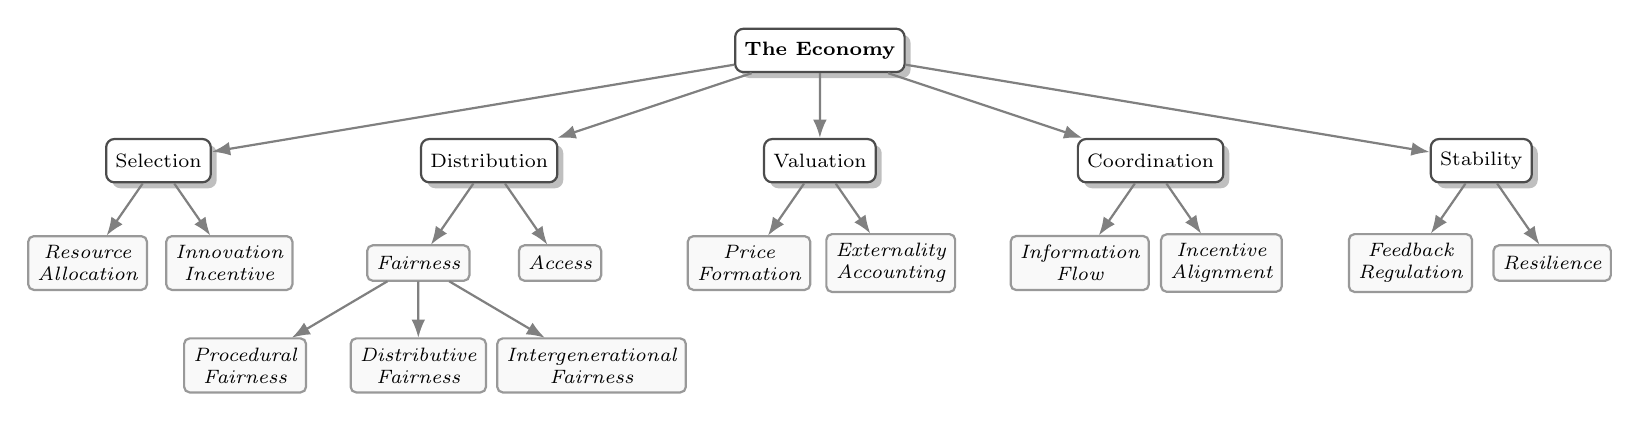
\begin{tikzpicture}[concepttree,
    level 3/.style={sibling distance=2.2cm, level distance=1.3cm}]
    \node[concept, font=\scriptsize\bfseries] {The Economy}
        child { node[concept] {Selection}
            child { node[leaf] {Resource\\Allocation} }
            child { node[leaf] {Innovation\\Incentive} }
        }
        child { node[concept] {Distribution}
            child { node[leaf] {Fairness}
                child { node[leaf] {Procedural\\Fairness} }
                child { node[leaf] {Distributive\\Fairness} }
                child { node[leaf] {Intergenerational\\Fairness} }
            }
            child { node[leaf] {Access} }
        }
        child { node[concept] {Valuation}
            child { node[leaf] {Price\\Formation} }
            child { node[leaf] {Externality\\Accounting} }
        }
        child { node[concept] {Coordination}
            child { node[leaf] {Information\\Flow} }
            child { node[leaf] {Incentive\\Alignment} }
        }
        child { node[concept] {Stability}
            child { node[leaf] {Feedback\\Regulation} }
            child { node[leaf] {Resilience} }
        };
\end{tikzpicture}}
\caption{Proposed conceptual decomposition of the economy, showing selected sub-concepts. White nodes are candidate axes; gray nodes are candidate sub-concepts that may recurse further, as the Fairness branch illustrates.}
\label{fig:economy-tree}
\end{figure}

This proposed carve treats the five axes as load-bearing, jointly covering the concept and analytically distinct although coupled in practice. It permits selection and distribution, and valuation and coordination, to be examined separately. Comparative decompositions can test whether those separations are useful or whether some axes should instead be merged.

The tree omits implementation actions such as raising interest rates, adjusting taxes, creating jobs, or building infrastructure. Those tasks emerge inside the conceptual structure: raising interest rates to stabilize an overheating economy calls on Stability $\to$ Feedback Regulation, while adjusting taxes to change the distribution of burdens calls on Distribution $\to$ Fairness $\to$ Distributive Fairness. Other purposes or coupled effects may call for additional contributions. The actions are economy-specific; the proposed conceptual axes are intended to recur across economic systems.

Now recurse one level. Distribution $\to$ Fairness decomposes into procedural fairness (is the process just?), distributive fairness (is the outcome just?), and intergenerational fairness (is it just across time?). Under this proposed carve, the dimensions are intended to satisfy necessity, independence, and universality. A \texttt{ProceduralFairnessSolver} defined by process justice could be called by economic system design, legal systems, hiring processes, hospital resource allocation, and school admissions. Its proposed transfer value comes from the recurrence of process-justice questions across those settings; whether a common Solver actually improves them remains to be measured.

\subsection{Example: Decomposing Education}

\begin{itemize}[leftmargin=1.5em]
\item \textbf{Content} (what is worth knowing?): knowledge selection, sequencing, relevance.
\item \textbf{Transmission} (how does knowledge transfer?): representation, interaction, scaffolding.
\item \textbf{Assessment} (how do you know learning occurred?): measurement, validity, feedback timing.
\item \textbf{Motivation} (why does the learner engage?): intrinsic drive, extrinsic structure, meaning.
\item \textbf{Adaptation} (how does instruction adjust?): diagnosis, differentiation, pacing.
\end{itemize}

\begin{figure}[H]
\centering
\resizebox{\textwidth}{!}{%
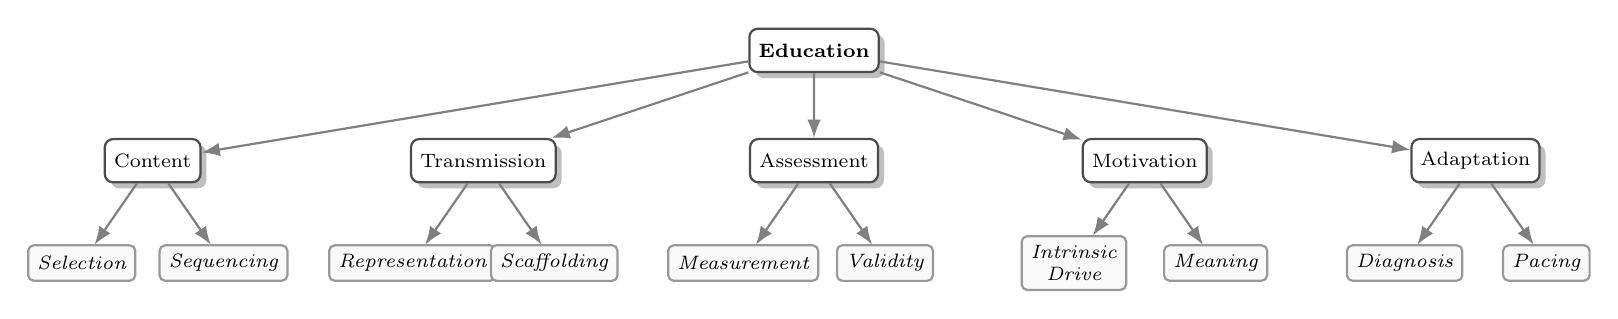
\begin{tikzpicture}[concepttree]
    \node[concept, font=\scriptsize\bfseries] {Education}
        child { node[concept] {Content}
            child { node[leaf] {Selection} }
            child { node[leaf] {Sequencing} }
        }
        child { node[concept] {Transmission}
            child { node[leaf] {Representation} }
            child { node[leaf] {Scaffolding} }
        }
        child { node[concept] {Assessment}
            child { node[leaf] {Measurement} }
            child { node[leaf] {Validity} }
        }
        child { node[concept] {Motivation}
            child { node[leaf] {Intrinsic\\Drive} }
            child { node[leaf] {Meaning} }
        }
        child { node[concept] {Adaptation}
            child { node[leaf] {Diagnosis} }
            child { node[leaf] {Pacing} }
        };
\end{tikzpicture}}
\caption{Proposed conceptual decomposition of education, with selected candidate reusable sub-concepts at depth two.}
\label{fig:education-tree}
\end{figure}

The proposed axes can vary across forms of education, while several sub-concepts suggest cross-domain correspondences. Assessment $\to$ Validity shares the question of whether a measure captures its target with medical diagnostics and software testing. Adaptation $\to$ Diagnosis may share a pattern of locating the relevant state with medical triage and debugging.

\subsection{Example: Decomposing Game Design}

\begin{itemize}[leftmargin=1.5em]
\item \textbf{Agency} (what can the player do?): action space, consequence, expression.
\item \textbf{Challenge} (what resists the player?): difficulty calibration, uncertainty, constraint.
\item \textbf{Feedback} (how does the player know their state?): immediacy, clarity, richness.
\item \textbf{Progression} (how does the experience change?): mastery curve, revelation, pacing.
\item \textbf{Coherence} (why does it hold together?): internal consistency, thematic unity, aesthetic integrity.
\end{itemize}

\begin{figure}[H]
\centering
\resizebox{\textwidth}{!}{%
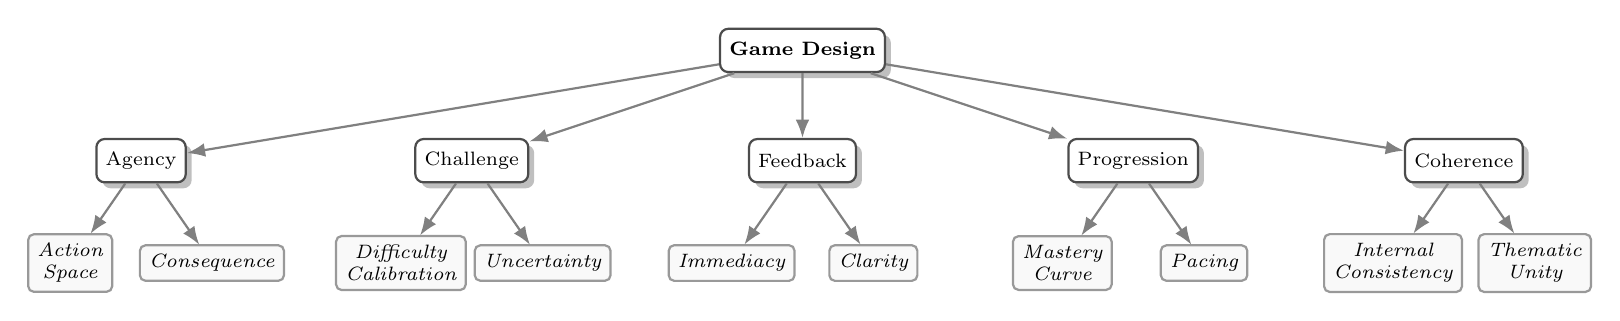
\begin{tikzpicture}[concepttree]
    \node[concept, font=\scriptsize\bfseries] {Game Design}
        child { node[concept] {Agency}
            child { node[leaf] {Action\\Space} }
            child { node[leaf] {Consequence} }
        }
        child { node[concept] {Challenge}
            child { node[leaf] {Difficulty\\Calibration} }
            child { node[leaf] {Uncertainty} }
        }
        child { node[concept] {Feedback}
            child { node[leaf] {Immediacy} }
            child { node[leaf] {Clarity} }
        }
        child { node[concept] {Progression}
            child { node[leaf] {Mastery\\Curve} }
            child { node[leaf] {Pacing} }
        }
        child { node[concept] {Coherence}
            child { node[leaf] {Internal\\Consistency} }
            child { node[leaf] {Thematic\\Unity} }
        };
\end{tikzpicture}}
\caption{Proposed conceptual decomposition of game design into five dimensions, with selected sub-concepts.}
\label{fig:game-tree}
\end{figure}

The proposed dimensions recur across chess, poker, tag, and digital games, although their prominence varies. Even low-challenge or sandbox forms contain agency, constraints, and feedback in attenuated forms. The sub-concepts may transfer as well: difficulty calibration shares structure with instructional pacing and progressive overload.

\subsection{Decomposing Intelligence Itself}
\label{sec:decompose-intelligence}

The operator should apply to its own target. What are the candidate differentiated dimensions of \emph{intelligence}?

No single decomposition is assumed canonical. Intelligence can be decomposed \emph{modally} (changing frames, working within them, bridging between them), \emph{structurally} (building a model, projecting it forward, evaluating outcomes, updating representations), \emph{functionally} (perceiving, acting, communicating), or in other ways. Different cuts may each be complete relative to a stated analytic purpose.

This paper's deepest claim is that intelligence should be modeled not only as a structure but as a process capable of restructuring its own representations in response to evidence. Fixed decompositions can support competence; adaptive restructuring is the additional capability of interest here. It allows a system to reshape the categories it uses for thinking when a problem exposes their limits.

Modular plant growth offers a biological analogy for topology-changing adaptation. Plants adjust to heterogeneous environments through distributed flows of resources and information, changing the persistent structure from which later growth proceeds~\cite{oborny2019plant}. Their form carries consequences of earlier responses and helps condition later ones. The analogy illustrates the difference between choosing actions within a comparatively stable organization and changing the organization through which future conditions are encountered; it is not evidence for the proposed machine architecture.

The proposed architecture instantiates this second mode through co-evolving topology (\S\ref{sec:substrate}), rejection-driven reframing (\S\ref{sec:seams}), ascent from depth (\S\ref{sec:jumps}), and convergence across paths (\S\ref{sec:topology}). The adjective \emph{fractal} refers to the pattern's recurrence across scales: a structure may compose into a larger one while remaining open to decomposition, retention, reuse, and revision.

Concrete decompositions remain useful as tools: modal cuts can assign roles, structural cuts can audit cognitive capacity, and functional cuts can reveal interface gaps. The adaptive-restructuring criterion within fractal intelligence is the capacity to adopt, revise, and discard such cuts as evidence and circumstances change.

\subsection{Cross-Domain Convergence: Why Reasoning Highways Form}
\label{sec:highway-selection}

Across these three domains, several candidate structural correspondences appear:

\emph{Feedback.} Assessment in education, feedback in game design, and feedback regulation inside economic stability each contain a narrower operation: using signals to estimate a system's state. A shared Solver would be justified only if constituent matching and probe routing showed that this operation is genuinely common.

\emph{Engagement.} Incentive alignment in economics and motivation in education may share operations involving intrinsic drivers, extrinsic structures, and meaning, while remaining distinct parent concepts.

\emph{Adjustment.} Adaptation in education and coordination in economics may both include sensing state, adjusting a path, and managing tempo.

\emph{Evaluation.} Validity in educational assessment, internal consistency in game design, and procedural fairness in economic distribution all compare system behavior against a governing criterion, but they remain distinct evaluative concepts.

The four tests explain the intended recurrence. By selecting for necessity, low coupling, universality over a declared range, and completeness relative to an outward capability, they favor abstract dimensions that are candidates for reuse beyond the problem that produced them. If those candidates capture real invariants, the uniform contract gives structurally similar problems a common destination regardless of origin domain. This is the selection account of highway formation; Section~\ref{sec:jumps} gives the ascent account, and Section~\ref{sec:reuse-measurement} the routing-and-credit account. Whether the candidates recur because they are found structure rather than attractive labels requires independent Root-only repetitions plus matched ablations that remove, scramble, or replace the upward-first and four-test operator.

Convergence creates the possibility of compounding, but two claims must be separated. \emph{Within-concept} compounding is a Solver improving through repeated instances of its own concept; the mandatory-abstraction construction records cross-problem and cross-domain structural reuse but not improvement, because it has no independent execution, Pathway Memory, acceptance gates, or outcomes (Section~\ref{sec:limitations}). \emph{Cross-concept} compounding, such as transferring what was learned about uncertainty in weather to finance, is the stronger and least certain extension. The empirical program is to map which concepts transfer, including negative transfer, rather than assume universal compounding.

\subsection{When Decomposition Goes Wrong}
\label{sec:decomposition-failures}

Two archetypal failures deserve attention. A \emph{leaky seam} looks clean on paper but implicit assumptions bleed across the boundary. If a \texttt{SelectionSolver}'s acceptance criteria embed a distributive objective, the distributive assumption has crossed the seam. The remedy is to strengthen the interface so the assumption must be explicitly typed. A \emph{misaligned cut} separates variables that must co-vary; the remedy is to revise or merge the boundary so the coupled variables are handled together.

The cost of a bad cut can be severe. If a parent solver makes a misaligned cut at the root, descendants may inherit a flawed ontology and optimize the wrong variables. The Frame Error mechanism (Section~\ref{sec:learning}) therefore allows leaf-node friction to challenge a parent decomposition. The mandatory-abstraction construction demonstrates higher-parent insertion and multi-parent topology, but its deterministic structural acceptance is not a feedback-triggered Frame Error or semantic repair (Section~\ref{sec:prototype-results}).

\subsection{The Stability of Solved Structure}
\label{sec:stability}

Two kinds of stability must not be conflated. A solved structure should remain addressable: its decomposition, execution route, outputs, gate results, provenance, and observed outcome should not evaporate when the task ends. But persistence does not make its decomposition canonical. The same problem may admit several useful carves, and later evidence may expose a seam that the incumbent missed. Stability belongs first to identity, retention, and learned reuse---not to one immutable ontology.

The architecture therefore separates three layers. An \emph{inclusive archive} retains evaluated solution graphs, including failed routes when they provide negative knowledge. A \emph{selective serving layer} promotes recurrent, validated, or niche-leading nodes and subgraphs into active infrastructure; Pathway Memory learns when to route through each. An \emph{experimental frontier} receives a bounded budget for fresh, convention-resistant carves when similarity is low, routing confidence is poor, frame errors recur, stakes are high, or an exploration schedule fires. Cheap carve sketches can be screened before full execution. This is a portfolio in memory: exclusion from the serving layer does not itself discard an archived alternative. Retention remains subject to permissions and the expiry and deletion requirements discussed in Section~\ref{sec:global}. Familiar problems normally exploit one evidence-backed incumbent rather than execute every retained carve.

Evaluated structures act like maintained roads: tasks generate traffic through them, recurrent routes can become highways, and failed routes can be bypassed or rebuilt. Reuse can amortize decomposition without making its cost disappear. Expected task cost is $C_{\mathrm{route}} + C_{\mathrm{solve}} + p_{\mathrm{explore}}C_{\mathrm{carve}}$: familiar tasks make the exploration probability small; novel or failing tasks make it larger. Whether retained structure lowers total cost enough to justify the archive, routing, and occasional re-carving is an empirical question. Matched-compute evaluation must charge every exploration call rather than declare the overhead negligible by construction.

\subsection{Evolutionary Encapsulation and Emergence in Reverse}
\label{sec:emergence}

For the purposes of this paper, complexity is observer-relative: it is the gap between a system's full internal detail and what an observer can meaningfully describe or hold in mind for the purpose at hand. An exact atomic-scale description of an ordinary macroscopic system is generally too detailed to track, even though compact laws capture many of its regularities. We make such systems cognitively workable through higher-level units such as cells, organs, organisms, and machines. Encapsulation does not remove internal complexity. It gives the system a bounded exterior through which it can participate in organization at another scale.

Natural intelligence is evolutionary in origin. Across major transitions in individuality, entities capable of independent replication became integrated into higher-level individuals. Cooperation, communication, division of labor, mutual dependence, and sufficiently low internal conflict allowed the collective to function as a new unit~\cite{west2015transitions,michod2007individuality}. This makes nested encapsulation an organizational precedent worth examining, not evidence that the Solver architecture works. Simon's stable-intermediate argument explains why such layering can make further complexification more tractable~\cite{simon1962}. Levin's multiscale-competency framework motivates the stronger cognitive hypothesis: cells, tissues, organs, and organisms can exhibit goal-directed competence at nested scales, with a collective presenting as one agent-like unit to the level above~\cite{levin2022tame}.

Seen through this precedent, the Solver architecture can be read as an engineered reversal of boundary assignment. Biological evolution supplies no a priori global contract: in some lineages, lower-level entities became integrated and a higher-level individual emerged. The architecture assigns the maximal boundary first: the \texttt{RootSolver} encapsulates the complete problem space of its deployment, and each submitted problem is selectively decomposed within it. Every child may contain a further Solver tree, yet a leaf and a compatible completed subtree can present the same contract boundary. Recursive closure therefore preserves encapsulation as an interface property. The proposed interface guarantees the form of the boundary, not that the boundary is conceptually correct, that its implementation is independent, or that the work behind it is good.

Contract-bounded Solvers serve as artificial cell-like units: a model, human, program, or team provides the cognitive interior; the contract provides the membrane, and the Manifest its compressed public description. A composite parent translates its obligation into child Tasks, inherited constraints, and acceptance criteria, then routes, synthesizes, and evaluates what returns. Its synthesis obligation is the local membrane contract: it states how the exact active child contributions, in their parent-local roles, plus routing, boundary management, integration, and evaluation realize the single outward capability promised above. A child may recur beneath many parents, remaining addressable while each assigns a different Task and role. Because a composite can itself serve as a child, the same whole--part relation nests recursively. Each composite Solver is thus both a whole relative to its children and a bounded component relative to its parent---what this paper calls \emph{constrained nested emergence}: the parent specifies conditions for coherence without prescribing every internal operation. Declared synthesis is inspectable evidence of a composition design, not proof that useful operational emergence occurred. Feedback may also update routing.

Conventional emergence begins with local entities and rules and yields a higher-order pattern that was not placed directly---flocking from boids, markets from traders, perhaps consciousness from neurons. The surprise is at the top: define the micro, and the macro may astonish. The proposed architecture reverses the direction of boundary assignment. It names the parent-level capability first, while leaving open which child configurations, cross-branch reuse, and routes will eventually sustain it: define the macro, and the micro may astonish. This inversion is why the paper uses the phrase \emph{emergence in reverse}.

That the contract is designed does not by itself disqualify this deliberately weak, operational sense of emergence. A cellular automaton's rules are written, but a glider need not be placed; what matters is whether the higher-order pattern arises from lawful interactions rather than being individually scripted. The analogous claim here is not that the system lacks constraints, but that no designer must specify in advance which compatible configurations persist, which nodes attract enough traffic to become reasoning highways, or how deep each branch will go.

The macro boundary is therefore assigned top-down, while useful routes, candidate higher parents, nodes that densify into highways, and the depth reached by each branch may emerge through use. There is no fixed architectural depth because any Solver may decompose again while remaining one unit to its parent. Every actual execution is nevertheless finite because it runs under a finite budget; the marginal-value rule decides whether further decomposition is worth spending that budget. The mandatory-abstraction construction does not yet establish this phenomenon: it derives a theory-conditioned scaffold and records declared composition rather than independent child action. It shows how the pattern can be represented, not that operational emergence occurred.

At the interface level, this can be read as selective decompression: the marginal-value rule decides where a bounded unit should expose additional internal reasoning. Retention and promotion perform the complementary abstraction by encapsulating recurrent working structure as a new addressable unit. The resulting design rule is to encapsulate a recurring structure when its public obligations are stable enough to name and test, while keeping the unit revisable. A system that never encapsulates risks being overwhelmed by its own interactions; a system that encapsulates too early risks freezing a carve that evidence has not yet earned. When recurrence makes generality earn its name, the structure becomes a candidate for sealing behind a hash (\S\ref{sec:sema}).

%==============================================================================
\section{A Theory of Depth}
\label{sec:ri}
%==============================================================================

Section~\ref{sec:algorithm} defines how to locate a problem upward and decompose it downward; this section governs how deep to go. At every node, the choice between direct solution and further decomposition, repeated across levels~\cite{parnas1972,babbage1832}, produces a \emph{solver tree} in which the same contract applies to workers and orchestrators. The \emph{Universal Solver Tree} is the aggregate of all such solver trees across agents in the system. Its universality concerns the intended breadth of problem coverage, not a uniquely correct ontology. Within each constituent tree, the root states the outward problem scope, while composition exposes the differentiated obligations and internal detail needed to fulfill it. A composition child need not be a subtype of its parent; specialization edges express that separate relation. This is the depth-wise counterpart of selective decompression: broad public claims at the root, selectively exposed detail below. When outcome evidence validates a distinction and later reuse demonstrates transferable value, retention can preserve it as accumulated structural intelligence. Depth alone is structural elaboration, not evidence of intelligence. The aggregate grows through vertical refinement by decomposition and lateral discovery by reframing, with the marginal-value rule deciding when additional depth is expected to pay.


\subsection{Selective Depth}
\label{sec:selective-depth}

Additional depth has costs and can bring diminishing returns, but a useful distinction may appear only after several refinements. Moreover, uncertainty is unevenly distributed. Uniform depth wastes budget on easy spans and starves the hard ones. The remedy is selective depth: concentrate refinement on sub-concepts with high uncertainty, brittle dependencies, or large impact. A \emph{hard seam} is a boundary whose failure could collapse the whole plan. Refining or repairing such a seam can prevent erroneous work from propagating through the subtree below it.

A solver tree provides explicit, asymmetric compute allocation: it can route inference budgets toward hard seams, resolve simpler spans shallowly, and retain an inspectable graph of work. The additional scaling axis proposed here is \emph{composition} across typed boundaries and trust domains, where invocation context can be separated and a detected failure can return a structured request for reframing.

Fractal intelligence can be instantiated by one model simulating a tree or by many specialized models (Section~\ref{sec:scale}). The relevant comparison is with systems that decompose implicitly: the wager is that making decomposition explicit, typed, and persistent enables reuse, localized learning, and cross-organization sharing.

The history of sports analytics illustrates this principle concretely. For decades, baseball evaluated players at a fixed granularity: batting average, runs batted in, earned run average. The Oakland Athletics under Billy Beane decomposed ``player value'' one level deeper---on-base percentage, slugging percentage, plate discipline---and discovered that conventional metrics were masking variables associated with wins. The next generation went deeper still: player-tracking systems decomposed movement into sprint speed, route efficiency, launch angle, spin rate, and defensive range. In the vocabulary of this paper, each variable becomes a candidate sub-concept with its own Solver, acceptance gate, and Pathway Memory. Baseball's unusually decomposable domain and rapid scoreboard limit generalization from the example. The marginal-value rule asks whether a proposed refinement is worth its incremental cost. Its threshold $\theta$ is not a fixed depth limit; another problem or later evidence may justify further detail. The wager is that conventional practice sometimes stops before examining refinements that would pay; Beane found leverage by analyzing player value at a finer conceptual resolution.

\subsection{The Marginal-Value Rule}
\label{sec:mvr}

The economic governor for depth is a ratio test whose lineage runs through information value theory~\cite{howard1966}, ecological foraging~\cite{charnov1976}, and rational metareasoning~\cite{Russell1991, Gershman2015}: deepen if and only if the expected improvement divided by the incremental cost exceeds a domain-appropriate threshold~$\theta$. Formally, at any node~$n$:

\begin{equation}
\frac{\mathbb{E}[V(n_{\text{deep}})] - V(n_{\text{shallow}}) + U(n)}{C(n_{\text{deep}}) - C(n_{\text{shallow}})} > \theta \,.
\end{equation}

Incremental cost includes the \emph{interface load} of an added boundary---translation, serialization, routing, synthesis, monitoring, and semantic loss---while the value term must credit any error or risk reduction that makes such friction worthwhile.

\noindent De Sabbata et al.~\cite{DeSabbata2024} applied this directly to LLM reasoning depth. This paper extends the principle from a single model's reasoning depth to a tree of contract-bounded solvers, governing not just how long to think but where to grow the hierarchy. The bonus term $U(n)$ is an exploration credit inversely proportional to the density of Pathway Memory at node~$n$, in the spirit of the upper-confidence-bound rule of Auer, Cesa-Bianchi, and Fischer~\cite{auer2002ucb}: nodes the system has rarely visited receive a temporary subsidy that converts the rule from pure exploitation into an exploration--exploitation trade-off, with the cold-start probe phase of Section~\ref{sec:cold-start} as its practical implementation.

In practice, an orchestrator implements this through a control loop:

\begin{figure}[H]
\begin{rfbox}
\small
\begin{verbatim}
ALLOCATE-DEPTH(branches, budget, theta):
  while budget > 0:
    ratios <- empty map
    costs  <- empty map
    for each branch b in branches:
      (dV, dC) <- b.Consult("estimate_next_step")
      ratios[b] <- dV / dC
      costs[b]  <- dC
    b_star <- argmax(ratios)
    if ratios[b_star] < theta:
      break
    b_star.Execute()
    budget <- budget - costs[b_star]
  return collect_results(branches)
\end{verbatim}
\end{rfbox}
\caption{The marginal-value rule as a control loop. The Consult surface makes the economic governor computable; the exploration credit $U(n)$ is omitted from the loop for clarity.}
\label{fig:mvr-loop}
\end{figure}

\noindent The Consult surface grounds its estimates in Pathway Memory rather than zero-shot self-evaluation (Section~\ref{sec:partition}). Each Solver maintains structured logs of past executions, recording which problem classes it has seen, what depths yielded improvement, and at what cost. A query like \texttt{estimate\_next\_step} returns a lookup: ``For problems structurally similar to this one, deepening with pattern Y has historically yielded a 12\% quality improvement at cost \$0.05.'' Where historical data is unavailable, the estimate defaults to a calibrated prior; when neither is available, the system allocates a fixed exploration budget to shallow probes before committing depth.

\subsection{Topology Freedom}
\label{sec:topology}

The contract constrains what crosses boundaries (typed artifacts and acceptance gates) but not how Solvers are arranged or sequenced. A task-oriented pipeline typically passes an \emph{instruction} (``do this specific thing''), which tends toward a fixed, sequential topology. A conceptual Solver passes an expression of \emph{intent} (``resolve this concept''). Because intent admits multiple fulfillment strategies, a parent need not prescribe the child's execution path; topology can instead adapt to observed evidence. Two persistent relation types must nevertheless remain distinct. A \emph{specialization} edge says that the child is a kind or realization of the parent and supplies an abstraction route. A \emph{composition} edge says that the child provides a differentiated contribution to the parent's outward capability and may become executable work. Node identity remains the capability contract; relationship meaning and parent-local role belong to the edge. The same contract supports radically different execution topologies:

\emph{Sequential chains}: output from Solver A to Solver B to Solver C.
\emph{Evidence-gated routing}: a parent examines a child's result and decides where to send it based on what the result contains---not based on its position in a sequence.
\emph{Fan-out and fan-in}: parallel solvers pursuing competing hypotheses, synthesized at a typed boundary.
\emph{Cycles}: a creative Solver and a verification Solver cycle repeatedly until the acceptance gate clears or the marginal-value rule halts.
\emph{Flat orchestration}: a parent routes among peers based on evidence, no tree depth.
\emph{Recursive nesting}: any of the above inside a single Solver that presents a single typed interface.

\noindent The term ``Universal Solver Tree'' names decomposition's rooted origin, not the final topology. One unchanged Solver may serve several parents, each supplying a typed \texttt{Task}, constraints, acceptance criteria, and edge-local role; reuse shares the capability, not the parent concepts or invocation contexts. Fan-in and multi-parent reuse therefore produce a directed graph, with $|E| > |V|-1$. The current reviewed concept-topology profile requires a rooted acyclic graph, even though bounded execution protocols may support cycles.

At each level, a parent's routing, synthesis, and evaluation are part of the intelligence under test. Manifest matching proposes compatible Solvers---one implementation could use vector similarity over declared Manifests---while Pathway Memory ranks them from prior evidence. Semantic similarity is a routing heuristic, not proof of contract compatibility. The conceptual structure is the blueprint, while each problem induces a route through it.

Topology freedom extends to the \emph{decomposition path} itself: for a given problem, the tree is not unique. Consider designing a city. One decomposition cuts by \emph{process} and elevates ``flow'' to a top-level sub-concept, with movement-in-homes appearing deep inside the flow branch. Another cuts by \emph{spatial object} and elevates ``buildings'' and ``streets'' at the top, with movement appearing twice in the tree---once inside buildings, once inside streets---without ever being decomposed as a first-order axis. Both decompositions may satisfy the four tests; neither is canonical. At the depth where movement appears, they may converge on the same \texttt{MovementSolver}: by importing its hash where the concept is adopted, or by semantic matching where it was independently derived. Content-addressing guarantees identity of adoption, not collision of derivation; that is the synonymy limit of Section~\ref{sec:limitations}. The hypothesis is therefore \emph{path-indifferent but concept-convergent}: it does not require one canonical tree, but predicts that useful atoms can recur across trees. Path-indifferent here means admissibility, not equal outcomes; the serving layer may learn that one carve helps more. The archive may retain both city graphs when they expose complementary structure.

This is the topological-identity angle of the adoption--discovery distinction; Section~\ref{sec:sema} states the semantic-matching limit, and Section~\ref{sec:reuse-discovery} the independent-reproduction test.

\subsection{Jumps and Reframing}
\label{sec:jumps}

This section gives the ascent account of highway formation, complementing selection in Section~\ref{sec:highway-selection} and routing-and-credit in Section~\ref{sec:reuse-measurement}.

When vertical decomposition bottlenecks---for example, when the marginal-value rule detects a flat improvement trajectory---more computation inside the same invariants may have little value. A lateral jump instead changes the frame so that a different region of solution space becomes locally available.

Alternative interpretations can themselves form a Discovery population (Section~\ref{sec:genreduce}). A \texttt{WhyChainSolver} searches beneath the stated problem, and a \texttt{ConstraintInversionSolver} tests inherited assumptions. Orthogonal Insight is one long-range variance operator available to that protocol: an unrelated seed is elaborated into a coherent causal world by a target-blind World Builder; a fresh Solver receives that world and the target; and a separate bridge compiles the operative relation into a real candidate mechanism~\cite{westerberg2025strangeworlds}. Orthogonal Insight calls the in-world step a \emph{Blind Solve}, meaning purpose blindness: the Solver receives the local target but not the experimental purpose or subsequent bridge task. The world changes what is locally ordinary before the system asks whether the resulting mechanism is useful.

Candidate reframings may then enter the companion ontology controller. Current occupancy and curator judgments can guide further commissions, while a later \texttt{ReduceSolver} could select candidates for downstream decomposability or present their trade-offs for user judgment. Automatic saturation detection and the reduction stage remain proposed controls.

The meta-perspective is maintained through parallel solvers at different levels of abstraction. Parent nodes see how the parts relate; children see how the parts work. Critically, this is bidirectional: a child solver may discover something that reshapes the parent's understanding---the Feedback surface is the channel through which children inform parents. A Frame Error at a child propagates upward as evidence for examining the parent's decomposition, not simply as a request to retry the child.

Mandatory classification ascent (\S\ref{sec:mandatory-abstraction}) is distinct from topology-changing ascent. Every case must locate itself on a specialization route; a new higher parent is added only when sibling comparison, recurrence, or a Frame Error supports a revised topology. This evidence-driven revision of the categories through which work is routed is \emph{ontological accommodation}. Reframing is thus not only lateral; it can also be \emph{ascending}. Topology-changing ascent has two independent triggers, only one of which is failure. The first is the Frame Error above: a child fails, and the failure supports investigating whether the parent's decomposition needs revision. The second is \emph{recurrence recognition}: a child succeeds, but while solving its sub-problem it recognizes that the conceptual structure it is handling is not specific to this branch at all---the same structure recurs across unrelated problems. Nothing has gone wrong; something general has been found. When that investigation or recurrence recognition identifies a reusable higher abstraction, the execution path does not merely descend the current branch; it \emph{teleports} to the newly recognized abstraction, where the pattern becomes a general concept with its own Solver. Subsequent problems encountering similar structure at any depth can now route directly to this elevated Solver, bypassing the decomposition that first discovered it. This is how reasoning highways (\S\ref{sec:reuse-measurement}) emerge at runtime: depth finds the pattern---through failure or through recurrence---ascent generalizes it, and future problems teleport to the generalization rather than re-deriving it. The trajectory through the tree is therefore not a monotonic walk but a graph traversal with occasional vertical jumps; depth and abstraction are coupled, not orthogonal.

%==============================================================================
\section{The Solver Contract}
\label{sec:contract}
%==============================================================================

The Solver Contract specifies how concept-defined abilities compose across boundaries. The distinction between Solver and agent is architectural: an agent is an implementation (a model, a program, a human), while a Solver is the interface that implementation presents to the system. The contract defines a five-surface namespace that may be implemented by a lightweight script, a frontier LLM, or a swarm of thousands. Manifest and Execute form the required core; Consult, Verify, and Feedback are discoverable extensions declared by the Manifest. ``Five-surface'' names the common interface vocabulary, not a claim that every lightweight Solver implements all five.

A Solver specializes through three complementary mechanisms: \emph{weight adaptation} (fine-tuning for a narrow problem class), \emph{tool composition} (invoking external capabilities), and \emph{execution harness} (a deterministic protocol guiding a general model through a domain-specific process). The contract is indifferent to which mechanism operates behind the interface. Section~\ref{sec:behind-solver} develops this opacity in detail: a single agent may implement many Solver contracts, a single Solver may orchestrate many agents internally, and the lifecycle from general-purpose hat to specialized system is governed by the same economic rule that governs depth.

The contract's intellectual ancestry is precise. Hoare~\cite{hoare1969} established verification through preconditions and postconditions. Meyer~\cite{meyer1992dbc} operationalized Design by Contract. Liskov and Wing~\cite{liskov1994} extended behavioral subtyping. Findler and Felleisen~\cite{findler2002} showed that contracts compose for higher-order functions---the recursive pattern Solvers require. The proposed extension here is that the boundary is not merely a validator but can return a typed request for upstream restructuring when the gate rejects. When that request changes the working carve rather than merely triggering another attempt, the boundary participates in ontological accommodation (Section~\ref{sec:jumps}). This states the architectural form of the boundary-as-contributor claim; Section~\ref{sec:synergy} gives its matched test, and Section~\ref{sec:boundary-formalization} its contrast with validator-only contracts. The five surfaces defined by the Solver Contract are shown in Table~\ref{tab:contract}.

\begin{table}[H]
\centering
\small
\caption{The five defined surfaces of the Solver Contract. Manifest and Execute form the required core; the other surfaces are discoverable extensions.}
\label{tab:contract}
\begin{tabular}{@{}llp{9cm}@{}}
\toprule
\textbf{Surface} & \textbf{Core Question} & \textbf{Purpose} \\
\midrule
Manifest & What can you do? & Declares the concept this Solver reasons about, its operations, input/output types, and any extended surfaces. Enables discovery and operation-level compatibility checks. \\
Execute & Can you do the work? & Takes a typed \texttt{Task}, returns a typed \texttt{Result}. The surface that performs conceptual work. \\
Consult & How would you approach this? & Open consultation: cost/quality estimation, clarification, rationale requests, context-sharing. Enables the marginal-value rule. \\
Verify & Why should I trust you? & Post-execution assurance: test vectors, reproduction recipes, verifiable evidence. \\
Feedback & How did you do? & Receives structured evaluation from downstream, or signals a Frame Error requiring a lateral jump. Enables localized learning. \\
\bottomrule
\end{tabular}
\end{table}

\noindent A \emph{core-compliant} Solver implements Manifest and Execute. An \emph{extended} Solver exposes any additional surfaces listed in its Manifest; a \emph{full-surface} Solver exposes all five. Compatibility is evaluated for the operation actually requested rather than inferred from a shared name.

\subsection{Gates That Redirect}
\label{sec:seams}

At each boundary between Solvers, three things happen: (1)~mode is declared (the Solver explicitly states its cognitive stance); (2)~output is typed (the artifact crossing the boundary has explicit structure); (3)~acceptance is gated (an \texttt{AcceptSpec} defines what must be true for the artifact to cross). The strictness of the gate scales with the seam. At soft seams (low-stakes internal handoffs), acceptance may be a lightweight shape check. At hard seams---structurally critical junctures or boundaries crossing trust domains---acceptance is non-compensatory: if any critical criterion fails, the artifact is rejected regardless of other scores.

These create \emph{seams that bite}~\cite{saltzer1984}: boundaries tight enough to maintain distinct cognitive modes, yet flexible enough to preserve internal freedom. Each gate acts as the endpoint of the subtree beneath it, judging that subtree's final artifact. The intended benefit of isolation is to reduce compromise among cognitive modes that would otherwise share one context.

Mode blending remains useful during divergent phases, where soft seams preserve permeable boundaries. Hard seams become relevant during convergence, when candidates must survive adversarial scrutiny. The \texttt{AcceptSpec}'s strictness is therefore a function of the cognitive phase.

\emph{Deterministic gates} evaluate mechanically decidable properties: schema conformance, hash matches, and unit tests. They avoid language-model evaluator error for those checks, but incomplete criteria and implementation defects can still produce false assurance. \emph{Probabilistic gates} rely on LLM evaluation. These inherit evaluator vulnerabilities: sycophancy, laziness, and \emph{evaluator collusion}---where generators and gate evaluators from the same model family share blind spots. A structural mitigation is to use adversarial evaluators at hard seams, potentially from different model families, ensemble juries, or dedicated red-team solvers. The proposed Discovery Protocol (Section~\ref{sec:genreduce}) therefore assigns generation and curation to distinct cognitive roles; whether model-family separation further improves reliability remains an empirical question.

A third outcome complements pass and reject: \emph{override-with-documentation}. When an artifact fails quantitative criteria but the failure reflects the limits of the criteria rather than the limits of the work, the gate permits passage with a typed justification citing what the criteria missed, why it matters, and how to test the override. This prevents deadlocking on problems where quantifiable criteria cannot capture everything. The Ethical Reasoning Protocol (Section~\ref{sec:prediction}) instantiates this mechanism.

The Solver Contract specifies a \emph{floor}, not a ceiling. The acceptance gate verifies the typed artifact (the minimum that must be true) but does not otherwise restrict supplementary material permitted by the Task's information boundaries. A solver can pass its full reasoning tree, rejected alternatives, and confidence distributions alongside the verified output---by reference rather than as raw text, so the receiver need not load everything at once. Material actually inspected still consumes context; the downstream solver selects what helps within its permitted view.

\subsection{The Transaction Model}

The fundamental interaction is a transaction. A Solver receives a \texttt{Task} object and returns a \texttt{Result} object:

\begin{table}[h]
\centering
\caption{The Task--Result transaction.}
\label{tab:transaction}
\small
\begin{tabular}{@{}lp{8cm}@{}}
\toprule
\textbf{Task Fields} & \texttt{operation}, \texttt{inputs} (typed), \texttt{constraints} (inherited obligations), \texttt{acceptance\_criteria} (\texttt{AcceptSpec}), \texttt{budget} (time/cost/compute limits) \\
\midrule
\textbf{Result Fields} & \texttt{outputs} (typed artifact), \texttt{status} (\texttt{success/partial/fail}), \texttt{stop\_reason} (\texttt{completed/budget/quality}) \\
\bottomrule
\end{tabular}
\end{table}

\noindent This forces handoffs to be structurally explicit. A Task payload crossing a hard seam:

\begin{figure}[H]
\begin{rfbox}
\small
\begin{verbatim}
{
  "operation": "sema:Optimize#0921",
  "inputs": {
    "mechanism": "Solid-State Battery Electrolyte",
    "target_metric": "ionic_conductivity"
  },
  "acceptance_criteria": {
    "schema": "sema:AcceptSpec#e4f1",
    "criteria": [
      {"metric": "conductivity_mS_cm", "comparator": ">=", "threshold": 1.0},
      {"metric": "thermodynamics", "status": "pass"}
    ]
  },
  "budget": { "max_compute_usd": 0.50 }
}
\end{verbatim}
\end{rfbox}
\caption{Example Task payload crossing a hard seam, with typed inputs, acceptance criteria referencing a Sema hash, and budget.}
\label{fig:json_payload}
\end{figure}

\noindent The \texttt{schema} field identifies the Sema definition used to interpret the acceptance criteria. Matching that reference establishes identity of the definition, not of the inline criterion values. Immutable agreement on the instantiated criteria requires a content reference that also binds those values, either directly or as part of the canonical Task contract. Identity and integrity do not establish that the criteria are correct or sufficient. The \texttt{status: partial} option supports anytime execution by allowing a Solver to return its best available intermediate result when it stops; returning that artifact does not itself mean that it has passed the caller's acceptance gate.

Figure~\ref{fig:sequence} illustrates a transaction across a hard seam, using the Consult and Feedback extensions when they are exposed by the Manifest.

\begin{figure}[p]
\centering
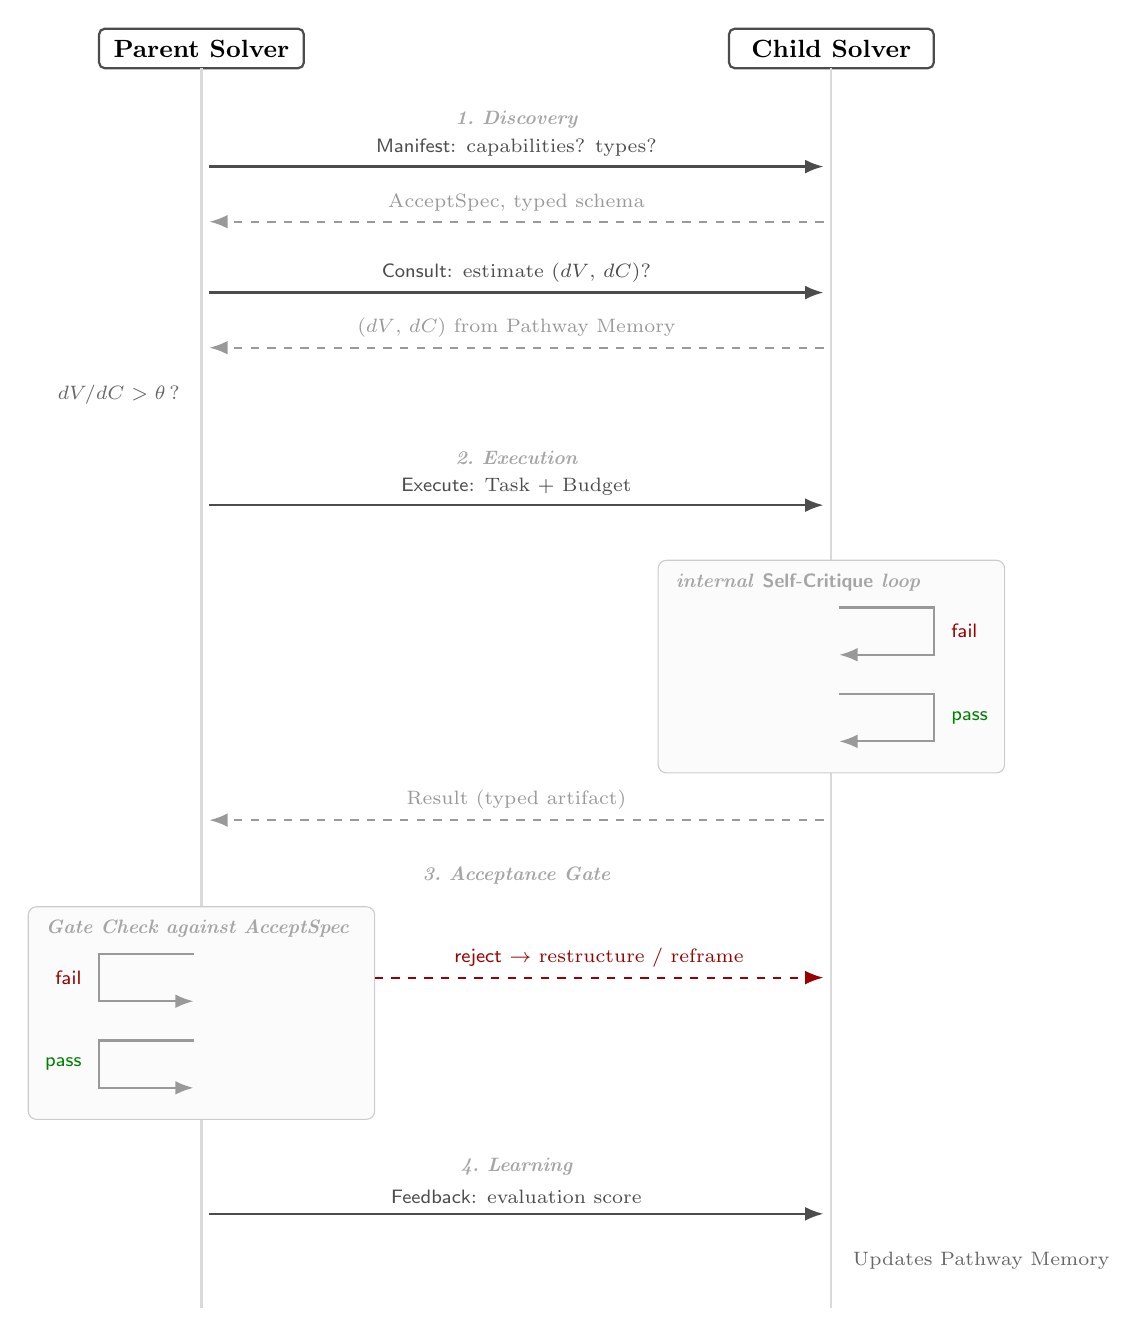
\begin{tikzpicture}[
    actor/.style={rectangle, draw=black!70, thick, rounded corners=2pt, minimum width=2.6cm, minimum height=0.5cm, align=center, fill=white, font=\small\bfseries},
    msg/.style={-Latex, thick, black!70},
    ret/.style={-Latex, thick, black!40, dashed},
    phase/.style={font=\scriptsize\bfseries\itshape, text=gray!70}
]
    \node[actor] (P) at (0, 0) {Parent Solver};
    \node[actor] (C) at (8, 0) {Child Solver};
    \draw[thick, gray!30] (0, -0.25) -- (0, -16.0);
    \draw[thick, gray!30] (8, -0.25) -- (8, -16.0);
    % Phase 1: Discovery
    \node[phase] at (4, -0.9) {1.\ Discovery};
    \draw[msg] (0.1, -1.5) -- node[above, font=\scriptsize] {\textsf{Manifest}: capabilities? types?} (7.9, -1.5);
    \draw[ret] (7.9, -2.2) -- node[above, font=\scriptsize] {AcceptSpec, typed schema} (0.1, -2.2);
    \draw[msg] (0.1, -3.1) -- node[above, font=\scriptsize] {\textsf{Consult}: estimate ($dV$, $dC$)?} (7.9, -3.1);
    \draw[ret] (7.9, -3.8) -- node[above, font=\scriptsize] {($dV$, $dC$) from Pathway Memory} (0.1, -3.8);
    \node[font=\scriptsize, anchor=east, text=black!60] at (-0.15, -4.4) {$dV/dC > \theta$\,?};
    % Phase 2: Execution
    \node[phase] at (4, -5.2) {2.\ Execution};
    \draw[msg] (0.1, -5.8) -- node[above, font=\scriptsize] {\textsf{Execute}: Task + Budget} (7.9, -5.8);
    \draw[rounded corners=3pt, gray!40, fill=gray!3] (5.8, -6.5) rectangle (10.2, -9.2);
    \node[phase, anchor=north west] at (5.9, -6.55) {internal \textsf{Self-Critique} loop};
    \draw[msg, black!40] (8.1, -7.1) -- (9.3, -7.1) -- (9.3, -7.7) -- (8.1, -7.7);
    \node[font=\scriptsize, text=red!60!black, anchor=west] at (9.4, -7.4) {\textsf{fail}};
    \draw[msg, black!40] (8.1, -8.2) -- (9.3, -8.2) -- (9.3, -8.8) -- (8.1, -8.8);
    \node[font=\scriptsize, text=green!50!black, anchor=west] at (9.4, -8.5) {\textsf{pass}};
    \draw[ret] (7.9, -9.8) -- node[above, font=\scriptsize] {Result (typed artifact)} (0.1, -9.8);
    % Phase 3: Acceptance Gate
    \node[phase] at (4, -10.5) {3.\ Acceptance Gate};
    \draw[rounded corners=3pt, gray!40, fill=gray!3] (-2.2, -10.9) rectangle (2.2, -13.6);
    \node[phase, anchor=north west] at (-2.1, -10.95) {Gate Check against AcceptSpec};
    \draw[msg, black!40] (-0.1, -11.5) -- (-1.3, -11.5) -- (-1.3, -12.1) -- (-0.1, -12.1);
    \node[font=\scriptsize, text=red!60!black, anchor=east] at (-1.4, -11.8) {\textsf{fail}};
    \draw[msg, red!60!black, dashed] (2.2, -11.8) -- node[midway, above, font=\scriptsize, text=red!60!black] {\textsf{reject} $\rightarrow$ restructure / reframe} (7.9, -11.8);
    \draw[msg, black!40] (-0.1, -12.6) -- (-1.3, -12.6) -- (-1.3, -13.2) -- (-0.1, -13.2);
    \node[font=\scriptsize, text=green!50!black, anchor=east] at (-1.4, -12.9) {\textsf{pass}};
    % Phase 4: Learning
    \node[phase] at (4, -14.2) {4.\ Learning};
    \draw[msg] (0.1, -14.8) -- node[above, font=\scriptsize] {\textsf{Feedback}: evaluation score} (7.9, -14.8);
    \node[font=\scriptsize, anchor=west, text=black!60] at (8.15, -15.4) {Updates Pathway Memory};
\end{tikzpicture}
\caption{Illustrative Solver transaction across a hard seam. Internal self-critique is one possible harness; Phase~3 is the caller's acceptance gate---the ``seam that bites.'' Rejection can prompt restructuring or reframing. A partial artifact may be returned for inspection without that return constituting acceptance.}
\label{fig:sequence}
\end{figure}

\subsection{Recursive Composition}
\label{sec:recursive-composition}

Any Solver may decompose its Task into sub-Tasks and delegate to child Solvers, applying the marginal-value rule at each level (Figure~\ref{fig:recursive}). Constraints are inherited fully and monotonically: if the root Task specifies ``no network access,'' every descendant inherits that constraint.

The Solver Contract is recursively closed in a structural sense: a composite subtree can present the same boundary as a leaf when the requested operation appears in its Manifest, the Task satisfies its declared input and constraint requirements, every descendant inherits constraints without weakening them, and the composite synthesis returns the declared Result type for evaluation against the caller's referenced \texttt{AcceptSpec}. These are operation-level conformance conditions rather than identity by label. They preserve interface-level encapsulation as the tree deepens but guarantee neither semantic equivalence, correctness, nor faithful execution; those remain the work of decomposition, typed specifications, gates, and outcome evaluation.

\begin{figure}[htbp]
\centering
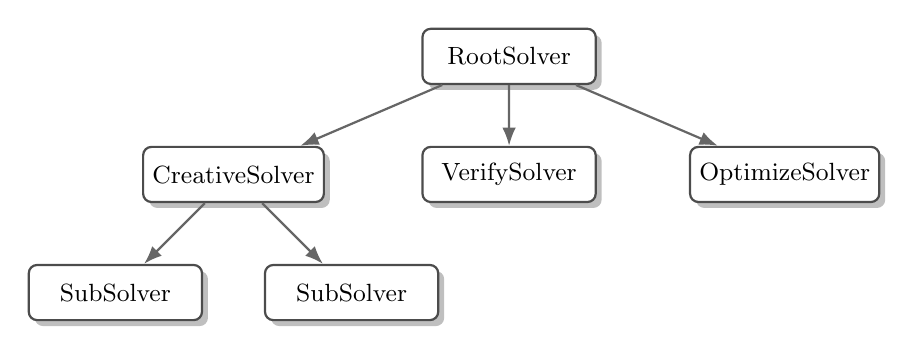
\begin{tikzpicture}[
    solver/.style={rectangle, draw=black!70, thick, rounded corners=3pt, minimum width=2.2cm, minimum height=0.7cm, align=center, fill=white, drop shadow, font=\small},
    level 1/.style={sibling distance=3.5cm, level distance=1.5cm},
    level 2/.style={sibling distance=3cm, level distance=1.5cm},
    edge from parent/.style={thick, -Latex, black!60, draw}
]
    \node[solver] {RootSolver}
        child { node[solver] {CreativeSolver}
            child { node[solver] {SubSolver} }
            child { node[solver] {SubSolver} }
        }
        child { node[solver] {VerifySolver} }
        child { node[solver] {OptimizeSolver} };
\end{tikzpicture}
\caption{Recursive decomposition. Each Solver may delegate to children, applying the same contract at every level. Depth is governed by the marginal-value rule.}
\label{fig:recursive}
\end{figure}

The apex case is the \texttt{RootSolver}: a Solver whose Task is an open-ended goal and whose cognitive operation is triage---determining what kind of problem this is and routing it. The \texttt{RootSolver}'s Pathway Memory is the architecture's most consequential site of compounding: it is the only node that sees how all problems enter the system.

The same boundary discipline can be expressed at five levels of ceremony\label{sec:scale}: (1)~natural language coordination, (2)~pattern-enriched dialogue using Sema patterns, (3)~lightweight Solvers with partial surfaces, (4)~rigorous Solvers with full contracts and non-compensatory gates, (5)~recursive orchestration with deep trees. Companion experiments suggest the largest gains may be front-loaded: the biggest reported improvement occurs between unstructured and pattern-enriched coordination~\cite{westerberg2026sema}. At the full-contract levels, the five surfaces provide a common interface for three coordination modes: \emph{hierarchical} (parent calls child), \emph{peer-to-peer} (Solvers with compatible extended endpoints engage directly), and \emph{stigmergic} (Solvers interact through a shared medium~\cite{westerberg2026understanding} rather than direct calls).

\subsection{What Sits Behind a Solver}
\label{sec:behind-solver}

The five-surface contract specifies what crosses the boundary, not what sits behind it. Whether a Solver is implemented by three models and a knowledge graph or by a bash script, the caller sees the same typed interface and judges it against the same \texttt{AcceptSpec}. This architectural opacity is deliberate and admits three deployment configurations:

\begin{itemize}[leftmargin=*]
\item \emph{One agent, many Solvers.} A single LLM instance registers multiple Manifests and activates the appropriate concept, bounds, and AcceptSpec based on the incoming Task. The solver tree is a conceptual structure, not a deployment topology---hundreds of conceptual nodes may be served by a handful of agents, each wearing many hats. This mirrors human organizations where a single expert fulfills multiple roles depending on context.
\item \emph{One Solver, many agents.} An \texttt{IncentiveAlignmentSolver} might internally route to a frontier model for novel mechanism design, a small fine-tuned classifier for known pattern recognition, and a Python script for game-theoretic equilibrium calculation. The caller sees one Solver presenting one Manifest. Behind it is a team. That internal organization may itself use conceptual decomposition, but it is invisible to the caller and governed by the Solver's own internal logic rather than the parent's routing decisions.
\item \emph{One Solver, one agent.} A dedicated fine-tuned specialist. The simple case.
\end{itemize}

A useful but limited property of the \emph{one agent, many Solvers} configuration is that the contract creates an explicit change of role. Generation and evaluation can run in fresh contexts under different Manifests and role-specific output contracts while retaining the same acceptance criteria for the artifact being judged. The model is then asked to reconsider that artifact against the declared criteria rather than continue the same generative trajectory. This may mitigate some same-trace self-correction failures, but shared weights and priors remain, so role separation does not guarantee independent judgment. It nevertheless provides a bootstrapping path: a frontier model can initially serve several concept-defined interfaces, while the resulting graph and evaluations remain addressable and individual nodes may later be replaced by specialized harnesses or models. An internal harness can also log and expose its steps; the contract's distinction is that exposed steps become typed, independently routable boundaries rather than remaining implementation details.

\subsubsection{The Solver Lifecycle}

This structural opacity admits a natural lifecycle. A Solver begins as a ``hat'' on a general-purpose LLM---no specialization, just the contract. As invocations accumulate and Pathway Memory reveals that a concept recurs across many domains, investment may become justified. The marginal-value rule compares the expected improvement from specialization with its cost, using invocation frequency and cross-domain breadth as evidence. A handful of uses may justify only a lightweight harness; frequent cross-domain use may justify fine-tuning or a dedicated model.

One possible specialization sequence unfolds structurally: an execution harness is added, then a fine-tuned classifier for routine cases, then domain-specific tools, and finally a full internal team. Recent work on Meta-Harness~\cite{lee2026metaharness} provides empirical evidence that this harness layer is load-bearing: automated optimization of the scaffolding around a single model produces accuracy improvements of 7--16 points, and this optimized harness transfers across different model architectures. In the architecture proposed here, Meta-Harness optimizes what sits behind one node; the contract governs how those nodes compose. The architecture produces the data that makes the decision to specialize legible.

\subsubsection{From Generalist Role to Specialized Solver}

A Solver may begin as a general model operating within a narrow semantic neighborhood. Its initial specificity comes from its conceptual role and position in the graph; execution harnesses, tools, and weight adaptation can strengthen it. For example, a \texttt{StabilityRegulationSolver} receives a typed subproblem isolated by upstream decomposition and emits an artifact filtered by an \texttt{AcceptSpec}. Repeated use may then justify progressively stronger specialization under the marginal-value rule. A prompted role can therefore develop into a specialized system when its invocation history supports the investment.

\subsection{Sema: Content-Addressed Concepts}
\label{sec:sema}

Collective thinking requires a shared repertoire of reusable cognitive strategies---patterns that prescribe \emph{how} to think about a class of problems, not merely what a concept denotes. Sema~\cite{westerberg2026sema} provides this by content-addressing pattern definitions: the cryptographic hash of a specification becomes its identifier, so two Solvers referencing the same hash are guaranteed to reference the same immutable specification---the same principle by which Git content-addresses code, applied to cognitive operations rather than source files. The hash guarantees identity of the canonicalized definition content only; interpretation, execution, and semantic discovery require additional mechanisms. Content identity needs no central registry, while discovering a compatible specification still depends on an unresolved semantic matching procedure; neither the construction artifact nor the reference implementation validates semantic equivalence. \emph{Semantic identity}---whether differently encoded specifications express the same operative invariants---is therefore an unresolved equivalence claim, not a property of the hash. Sema patterns supply a shared, content-addressed vocabulary for the architecture's components and supporting operations (Table~\ref{tab:mapping}); the broader Solver surfaces may combine several such patterns behind one interface.

This is the semantic-retrieval angle of the adoption--discovery distinction; Section~\ref{sec:topology} gives its topological consequence, and Section~\ref{sec:reuse-discovery} its empirical test.

Not every cognitive artifact should become a Sema pattern. A hash can in principle be minted over anything---a specific chain of reasoning, a single day's deliberation, an idiosyncratic problem decomposition---but like words, cognitive patterns gain \emph{infrastructural value through generality}. A one-off pattern can still be worth preserving, but repeated use across domains spreads the cost of defining and checking it while creating opportunities for further improvement. This mirrors the Universality criterion of the decomposition algorithm (\S\ref{sec:algorithm}): good sub-concepts, and good Sema patterns, are the ones that recur. The complement holds on the other side: the Understanding Graph~\cite{westerberg2026understanding} stores specific instances of thinking---narrative traces of reasoning toward a particular understanding. When a recurring structure is recognized in such traces, it may be promoted into a Sema pattern. The promotion is the same ascent mechanism described in \S\ref{sec:jumps}, but across memory systems: specific-thinking (Understanding Graph) matures into reusable-strategy (Sema) when recurrence makes generality earn its name.

\begin{table}[h]
\centering
\caption{Representative Sema patterns supporting architectural components and operations. A supporting pattern need not implement the full surface named in the first column.}
\label{tab:mapping}
\small
\begin{tabular}{@{}llll@{}}
\toprule
\textbf{Concept} & \textbf{Sema Pattern} & \textbf{Hash} & \textbf{Role} \\
\midrule
\multicolumn{4}{@{}l}{\textit{The Solver Contract (Five Surfaces)}} \\
\quad Manifest & \texttt{Card} & \texttt{\#f1e1} & Capability advertisement \\
\quad Execute & \texttt{CognitiveSolver} & \texttt{\#c9f9} & Universal solver atom \\
\quad Consult & \texttt{SocraticLoop} & \texttt{\#4c98} & Pre-execution consultation \\
\quad Verify & \texttt{Validate} & \texttt{\#c745} & Schema verification \\
\quad Feedback & \texttt{PerformanceSignal} & \texttt{\#db20} & Downstream evaluation \\
\midrule
\multicolumn{4}{@{}l}{\textit{Proposed Architectural Mechanisms}} \\
\quad Good Cuts & \texttt{Decompose} & \texttt{\#7ee9} & Conceptual splitting \\
\quad Selective Depth & \texttt{RecursionDive} & \texttt{\#9db4} & Vertical tree traversal \\
\quad Marginal-Value Rule & \texttt{MarginalValueRule} & \texttt{\#ee80} & Economic stop-condition \\
\midrule
\multicolumn{4}{@{}l}{\textit{Infrastructure}} \\
\quad Task & \texttt{Task} & \texttt{\#d9f9} & Atomic unit of work \\
\quad Result & \texttt{Solution} & \texttt{\#084c} & Typed output artifact \\
\quad AcceptSpec & \texttt{AcceptSpec} & \texttt{\#e4f1} & Typed acceptance boundaries \\
\quad Solver Tree & \texttt{UniversalSolverTree} & \texttt{\#0715} & Collective knowledge graph \\
\bottomrule
\end{tabular}
\end{table}

Sema is a library of over 450 specialized thinking strategies, including \texttt{SocraticLoop} (clarification before generation), \texttt{SteelmanCheck} (mandatory counter-argument), and \texttt{PreMortem} (failure simulation). These procedural patterns can serve as executable specifications for a consuming Solver: they describe mechanisms, invariants, preconditions, failure modes, and typed dependencies that a harness may interpret as scaffolding. Hydration loads the definition and its dependencies; the Sema server supplies them as data rather than executing their behavior. In the proposed architecture, the consuming Solver's harness performs the steps and applies available mechanical or model-based checks to the declared invariants. Content-addressing prevents unnoticed changes to the hashed canonical definition: a change to that content produces a different identifier, although execution can still diverge. Refinement therefore lives \emph{behind} the hash, not inside it: the specification is immutable while the Pathway Memory and harnesses behind it may improve (the skeleton--muscle split of Section~\ref{sec:global}); a change to the specification itself is a new version, and version migration at scale remains open.

Content-addressing provides three properties useful for collective thinking. \emph{Specification identity}: matching hashes imply matching canonical specification bytes, not merely matching function signatures. \emph{Granular negotiation}: if fields are independently addressed in a Merkle tree, Solvers can agree on one referenced component while disputing another. \emph{Immutable reference with mutable organization}: hashed fields are immutable under a given identifier, while unhashed metadata can be reorganized without changing that identifier. These properties establish stable reference, not shared interpretation or correct execution.

\subsection{Productive Extremes}
\label{sec:synergy}

Structural separation may protect cognitive modes that interfere when co-activated. Like a cell membrane, a typed boundary permits unlike processes to coexist while preserving their distinct operating conditions. Dual-process research~\cite{kahneman2011,stanovich2000,evans2008dual} reports such interference in human cognition: analytical verbalization can disrupt insight problem-solving~\cite{schooler1993}, deliberate thought can suppress divergent generation~\cite{dijksterhuis2006}, and dual-task interference degrades performance even in simple tasks~\cite{pashler1994}. Related effects appear in language models: task-switching within conversational history can degrade performance~\cite{Gupta2024interference}, generalist multimodal models may underperform specialists under objective interference~\cite{MoME2024}, and outputs can regress toward the mean in creative tasks~\cite{GaltonMedian2025}. A concurrent analysis spanning 152 findings across agent prompt architectures catalogs 21 labeled interference patterns and argues that ``the agent that resolves the conflict cannot be the agent that detects it''~\cite{Arbiter2026}. Together, these findings motivate the hypothesis that interference can become a structural limitation and that typed conceptual boundaries may mitigate it; they do not establish that such boundaries are the only remedy.

The defining test is whether boundaries between concepts produce results unavailable to an individual model under matched prompting, sampling, memory, and compute. If they do, the boundary is not only a validator but an \emph{intelligence contributor}: its separation and typed exchange change the reachable result. Released Orthogonal Insight artifacts illustrate target-blind world construction, purpose-blind in-world solving, and extraction, while the companion Ontology study documents curator-driven redirection~\cite{westerberg2025strangeworlds,westerberg2026ontology}. Existing artifacts illustrate these ingredients but leave the defining comparison open because they lack a matched monolithic baseline and independent coding of mechanism novelty. A machine system could maintain dozens of competing hypotheses or alternative causal worlds in parallel, beyond an individual's working memory, while the uniform contract makes their artifacts composable. This is an architectural capacity, not a result established by the current studies.

Here the architectural claim of Section~\ref{sec:contract} becomes an empirical test; Section~\ref{sec:boundary-formalization} supplies the related-work contrast.

\subsubsection{Illustrative Trace: Orthogonal Insight}

To see the proposed mechanism in concrete form, consider a released Orthogonal Insight trace, later analyzed in the companion Ontology study~\cite{westerberg2025strangeworlds,westerberg2026ontology}. The problem: design a retirement system for variable-income workers. Three separately prompted phases use asymmetric information boundaries.

\emph{Phase~1: World-Building.} A World Builder, given the seed word ``theatrical,'' constructs an alien physics with no knowledge of the downstream problem. In the resulting world, causality follows narrative logic: nothing becomes real until it is witnessed, events resolve at the moment of maximum dramatic impact, and the fundamental force is not gravity but \emph{Tension}, the pressure of unresolved dramatic potential.

\emph{Phase~2: Blind In-World Solving.} The in-world Solver is purpose-blind: it receives the retirement problem and generated world, while the experimental rationale and later extraction task are withheld. Because the runner forwards the generated world verbatim, the seed word may remain visible; the information barrier concerns experimental purpose rather than seed identity. Working as though theatrical physics were real, the Solver designs a Tension Ledger tracking ``dramatic weight'' rather than dollars, Contribution Ceremonies where sincerity matters more than amount, and Timing Guilds that read narrative readiness rather than account balances. Coin and pooled funds still exist in the fictional world, but balance no longer governs retirement; dramatic weight, sincerity, and narrative readiness do.

\emph{Phase~3: Extraction.} A third Solver translates back to reality. ``Tension Ledger tracking dramatic weight'' becomes a hardship-adjusted sacrifice score: contributing 5\% of income when income has dropped 40\% scores higher than contributing 10\% at stable income. The resulting design, Witnessed Sacrifice Retirement, inverts standard retirement logic entirely, measuring what it cost you to save rather than how much you saved.

The trace makes the search hypothesis concrete: world construction changes the premises before in-world solving, and a fresh extractor compiles the resulting relation back to reality. It illustrates the hypothesis rather than testing causal superiority; the study lacks a compute-matched monolithic baseline and does not isolate phase separation.

The companion study also implements population-level curation. Its execution harness assigns proposal generation to fresh Explorers and confines the recurring Taxonomist---modeled here as a \texttt{TaxonomistSolver}---to classification, admission, redirection, and restructuring of a persistent typed graph. The graph database functions as an external cognitive prosthetic: no uninterrupted Taxonomist context must remember the whole population, yet each session can inspect and revise its represented structure. When the Taxonomist rejects with a structural diagnosis and commissions a mechanism-changing retry, this paper calls the operation \emph{structural coaching}; when a candidate does not fit the current categories and the graph itself changes, it is ontological accommodation. One trace moves a retry from detection-to-trigger toward ownership routing. Another adds \emph{Reframe Inconsistency} after judging a candidate outside seven existing top-level stances. These records establish executed redirection and category revision, not their causal effect on creativity or recovery of a natural ontology.

\subsubsection{Isolation vs.\ Self-Similarity}

Purpose separation can be implemented through ordinary sequential API calls and careful system prompts. The contract contributes a uniform structure for composition and retention: evaluated trees can persist as solution graphs, recurrent structures can be promoted into content-addressed patterns, and the Consult surface, typed gate outcomes, and Pathway Memory make depth decisions, local evaluation, and later routing first-class architectural objects (Sections~\ref{sec:sema} and~\ref{sec:mvr}). Isolation supplies the cognitive mechanism; self-similarity and persistence make it recursively composable and reusable.

\subsubsection{Structural Reliability and Safety}

This architecture aims to move some safety burden from generation weights to explicit boundaries~\cite{Huang2025}. It targets one possible \emph{alignment tax}: capability lost when generation and safety evaluation must compromise inside the same cognitive process. Where a gate can evaluate the relevant hazard, generation and verification need not be optimized in the same context. This may reduce one source of capability--safety compromise, but it does not make safety a property of the boundary alone; the result remains limited by the gate's coverage, evaluator quality, and the behavior of the underlying Solvers (Section~\ref{sec:limitations}).

A strict gate introduces a mechanical risk: deadlock in a rejection spiral. Repeated rejection may indicate a flawed decomposition, an unattainable or badly specified criterion, or evaluator error. After $N$ materially similar rejections, the marginal-value rule can halt leaf retry and request diagnosis at the parent boundary: revise the carve, revise the criterion with documented authority, or stop (Section~\ref{sec:jumps}). If no justified repair clears the gate, the anytime property activates: \texttt{status: partial} with the best intermediate result available.

Where Solvers have isolated parameter sets, fine-tuning one does not alter another's parameters. This prevents updates in one Solver from causing catastrophic interference in unrelated Solvers, though it does not prevent forgetting within an individual Solver~\cite{mccloskey1989}. The creative Solver need not be trained directly against the verifier's objective, but pretrained knowledge or supplied context may still let it anticipate the criteria; parameter separation reduces cross-objective interference rather than guaranteeing cognitive purity. The unit of training shifts: instead of one large generalist, one may train a portfolio of specialists whose value comes from how they compose through the contract.

The contract can improve structural reliability by catching some failures before they propagate. Under an illustrative independence assumption, a ten-step chain of 90\%-reliable Solvers yields 35\% end-to-end success ($0.9^{10} \approx 0.35$). Acceptance gates can stop detected failures, but end-to-end reliability remains limited by both Solver error and gate coverage, including false accepts and false rejects. A typed boundary can similarly contain a prompt injection only when the compromised output violates a criterion the gate can verify; a malicious but well-typed artifact may still pass. The boundary is therefore a partial firebreak, not a security guarantee. A companion demonstration supports the narrower coordination claim: in a multi-agent trading swarm, natural-language coordination produced catastrophic loops with fat-tail latency (up to 51 turns and 317~seconds), while the reported protocol condition had median 15.4 turns and 203~seconds with no observed fat tail~\cite{westerberg2026sema}. The comparison does not isolate which protocol component caused the difference.

%==============================================================================
\section{Localized Learning}
\label{sec:learning}
%==============================================================================

The proposed architecture supports learning at four levels. First, each node can accumulate Pathway Memory---performance data from its invocations---to ground later marginal-value estimates and routing decisions. Second, a node may sharpen at its specific job through fine-tuning, tool integration, harness refinement, or better estimates from experience. Third, observed divergence or redundancy can motivate splitting, merging, or reparenting nodes. Fourth, routing models can learn which paths work for which problem types, co-evolving with the specialists they route to. Conceptual identities remain addressable while the topology and the capabilities behind them remain open to revision.

\subsection{Partition by Subproblem Type}
\label{sec:partition}

When an acceptance gate detects a failure at a seam, the responsible Solver boundary becomes an explicit unit for diagnosis and localized feedback.

When evidence suggests that a Child Solver is failing because the Parent made a leaky cut rather than because of the child's own limitations, the Feedback surface can return a \emph{Frame Error}. This requests parent-level diagnosis and may trigger the lateral jump of Section~\ref{sec:jumps} instead of another leaf retry.

The diagnostic question is when to declare a Frame Error rather than retry the leaf. The proposed Feedback policy treats two patterns as \emph{insolubility signatures}. \emph{(A)~Convergent failure under structural diversity}: when several sub-solvers built on materially different internal mechanisms (different harnesses, parameter families, or tool sets) all violate the same \texttt{AcceptSpec} clause, repeated agreement becomes evidence of an upstream ontological leak, although leaf noise and gate error remain possible. \emph{(B)~Oscillatory constraint contradiction}: when outputs satisfying clause~$A$ repeatedly break clause~$B$, and vice versa, the parent may have posed an impossible problem. Either pattern can request a lateral jump (Section~\ref{sec:jumps}) after the specified evidence threshold. To prevent indefinite reframing, both signatures are governed by an \emph{ontological cooling} schedule: as compute budget drains or the reframing taxonomy of Section~\ref{sec:jumps} saturates, the trigger threshold rises monotonically, so the system can stop or return partial work rather than loop indefinitely inside the meta-loop. Exhausting the budget does not itself justify the override-with-documentation mechanism (Section~\ref{sec:seams}); an override still requires the stated justification that the criteria miss something material.

Localized learning rests on a distinction the contract makes structurally explicit: \emph{protocol transfer} versus \emph{weight transfer}. Protocol transfer distributes one immutable protocol identity---the decomposition graph, public acceptance clauses, and gate structure identified by a Sema hash---but byte-identical content does not establish that the protocol will transfer successfully across domains. Weight transfer, or local weight adaptation, changes parameters and can instead be scoped to a single Solver's execution boundary: LoRA-style fine-tuning~\cite{hu2022lora} need not update unrelated parameter sets. The typed Task is intended to act as a semantic bottleneck, with an upstream node translating a domain-specific payload (currency reserves, affect state) into the abstract variables the specialist expects and a downstream node translating its output back into domain language. Whether this bottleneck adequately limits domain-vocabulary contamination is empirical. This realizes the function--arguments analogy of Section~\ref{sec:concept-context}: the hash fixes the function specification; the arguments vary by invocation.

Alongside the specialization mechanisms of \S\ref{sec:behind-solver}, \emph{Pathway Memory} records explicit performance data (quality, depth, cost) across problem classes and grounds the marginal-value estimates. It may use a typed reasoning-capture graph~\cite{westerberg2026understanding} or a leaner statistical index optimized for routing speed. The standardized Feedback surface supports three timescales: \emph{immediate} rejection data, \emph{medium-term} pathway attribution, and \emph{long-term} real-world outcomes.

\subsection{Reasoning Highways and Credit Assignment}
\label{sec:reuse-measurement}

The credit assignment problem---determining which node in a deep hierarchy caused a downstream failure---is typically the hardest obstacle to learning in hierarchical systems. The Solver architecture localizes evidence by accumulating outcomes at common nodes, supporting conditional performance estimates and targeted comparisons. This makes \emph{local} credit assignment more tractable without making every association causal; counterfactual routing comparisons may still be needed. \emph{Global} routing credit assignment remains an open challenge (Section~\ref{sec:limitations}).

When structurally diverse problems route through the same conceptual decomposition nodes, each node can accumulate a frequentist signal without explicit weight training. These convergent paths---\emph{reasoning highways}---would form when the routing layer sends structurally similar conceptual sub-problems to the same specialists across origin domains. A \texttt{DistributionSolver} handling tax-policy allocation, network bandwidth routing, and scholarship allocation would generate localized performance records through use: the same node is observed across different inputs and outcomes. These are comparable observations rather than controlled experiments.

This is the routing-and-credit account of highway formation; Sections~\ref{sec:highway-selection} and~\ref{sec:jumps} give its selection and ascent accounts.

Reasoning highways share \emph{Sema scaffolding}---the conceptual decomposition, acceptance gates, and sub-solver types---while domain-specific payloads may be handled by separate node instances. The routing model learns the structural correspondence among those instances: tax-policy allocation and scholarship allocation may decompose into the same conceptual sub-problems without overloading one node with both domains.

The reuse cycle requires problems to route through genuinely common conceptual structures; the contract makes reuse composable and outcomes comparable, but does not guarantee independent convergence (Section~\ref{sec:limitations}). In a decentralized commons, the backward learning flow also needs protection from fabricated penalties. A \emph{Receptivity Gate}\label{sec:receptivity} requires a rejecting parent or caller to submit a typed \texttt{FailureTrace} naming the violated \texttt{AcceptSpec} clause; the child or producing Solver verifies the trace before accepting the feedback, and invalid or hallucinated feedback is dropped.

%==============================================================================
\section{Generalized Decomposition Protocols}
\label{sec:discussion}
%==============================================================================

This section presents ten generalized protocols: nine author-designed decompositions of recurring cognitive needs and one General Problem-Solving Protocol derived by applying the four-test algorithm to problem-solving itself (Section~\ref{sec:general-protocol}).

Each protocol is intended as a cross-domain decomposition of a recurring cognitive need. Its specification abstracts away the domain payload, although its chosen boundaries and examples may still encode assumptions inherited from the author or model. Each extends chain-of-thought reasoning across contract-bounded Solver invocations, whether implemented by one model or many: Chain-of-Thought~\cite{wei2022} made reasoning linear, Tree-of-Thoughts~\cite{yao2023} made it branching, and these protocols make it boundary-separated and persistent. Domain knowledge enters through the Solvers and contexts invoked within a protocol. Because the protocols attach to recurring concepts rather than one prescribed application domain, they are candidates for the architecture's highest reuse tier rather than proven domain-agnostic structures.

The nine specialized protocols are design proposals rather than outputs mechanically generated by the algorithm. The formalization in Section~\ref{sec:algorithm} attempts to systematize the intuitive process that produced them.

Several protocols below contain an inherent causal order: prediction precedes scoring, and interpretation precedes planning. Their decomposition nevertheless concerns continuous, co-constraining faculties rather than chronological tasks. The temporal sequence follows data dependency; matched tests must determine whether separating the faculties reduces interference (Section~\ref{sec:synergy}).

Ten recurring cognitive needs, ten proposed protocols:

\begin{itemize}[leftmargin=1.5em]
\item \textbf{Producing with quality}: Collaborative Writing (Section~\ref{sec:writing})---``Does this meet the standard?''
\item \textbf{Understanding people}: The Human Emulator (Section~\ref{sec:hep})---``How should I respond to this person?''
\item \textbf{Evaluating}: PURE (Section~\ref{sec:pure})---``Is this worth pursuing?''
\item \textbf{Discovering}: The Discovery Protocol (Section~\ref{sec:genreduce})---``What are the best solutions from a diverse field?''
\item \textbf{Predicting}: Temporal Ensemble Forecasting (Section~\ref{sec:thl})---``What will happen?''
\item \textbf{Choosing rightly}: Ethical Reasoning (Section~\ref{sec:prediction})---``What is the right thing to do?''
\item \textbf{Verifying}: The Truthseeking Protocol (Section~\ref{sec:truth})---``Is this true?''
\item \textbf{Making}: The Creation Protocol (Section~\ref{sec:maker})---``How should this be brought into existence?''
\item \textbf{Solving}: The General Problem-Solving Protocol (Section~\ref{sec:general-protocol})---``What is any problem made of?''
\item \textbf{Self-regulating}: Meta Protocols (Section~\ref{sec:meta-protocols})---``Is the system still the right shape?''
\end{itemize}

\subsection{Collaborative Writing: Decomposing the Concept of Textual Quality}
\label{sec:writing}

The protocol decomposes the concept of \emph{quality-constrained production}---what it means to produce something to a standard---into five intended low-coupling dimensions: \emph{substance} (what material must the artifact contain?), \emph{structure} (how does it organize?), \emph{generation} (produce freely, with evaluation elsewhere), \emph{evaluation} (does it meet the standard, across independent quality dimensions?), and \emph{refinement} (surface quality on a structurally complete artifact).

Writing makes the decomposition vivid because most of its cognitive work is invisible. A single sentence in a scientific paper activates an entire evaluative apparatus in any trained reader~\cite{westerberg2026entangled}, and the writer performs these evaluations silently, in parallel, each one bleeding attention from the others. The imperative to be precise suppresses vividness. The awareness of audience dampens technical depth. Conventional task delegation reproduces this: the writer still self-censors during generation while the editor catches style, logic, and structure in a single read.

The protocol separates structural production from concurrent monitoring. In the production path, a \texttt{ScopeDiscoverySolver} identifies every distinct idea the text must teach---ideas rather than sentences---and produces a flat list. A \texttt{SequencingCoherenceSolver} orders them by dependency. A \texttt{UnitConstraintSolver} writes one paragraph per idea, while a \texttt{StructuralVerificationSolver} checks the argument scaffold for unsupported claims, orphaned examples, and mechanisms disconnected from the claims they are meant to explain. A \texttt{VoiceRefinementSolver} adds connective tissue to the structurally complete document. The marginal-value rule governs further decomposition, from a short memo that stops at one paragraph per idea to a high-stakes argument that spawns sub-solvers for units needing deeper treatment.

Concurrent monitors externalize otherwise implicit evaluation. Multiple \texttt{ObserverSolvers}---a \texttt{RepetitionSolver}, a \texttt{ContradictionSolver}, an \texttt{IntentSolver}, and an \texttt{AudienceReceptionSolver}---receive the evolving artifact and return typed annotations describing location, severity, and the cognitive mode that triggered the signal. They annotate rather than rewrite, separating evaluation from revision. No extension to the Solver Contract is required: an \texttt{ObserverSolver} is a standard Solver whose Task is the current artifact state and whose Result is a set of typed annotations.

A \texttt{TextCategorizationSolver} assigns each paragraph a conceptual type---definition, mechanism, example, property, motivation, claim---and flags patterns such as several consecutive paragraphs performing the same rhetorical function for review of what each contributes. Repeated functions can be necessary; the question is whether they develop the argument or duplicate it. This operates on the concepts underneath the text rather than on surface wording alone.

The proposed observers illustrate all three specialization mechanisms. A \texttt{RepetitionSolver} equipped with a sentence-level embedding index can perform pairwise cosine similarity across every paragraph: \emph{tool use}, moving a suitable comparison outside the language model. A \texttt{StructuralCoherenceSolver} can walk a deterministic checklist (does every forward reference resolve? is every concept introduced actually used?): an \emph{execution harness}. A \texttt{ContradictionSolver} could be fine-tuned for greater sensitivity than a generalist prompted to ``check for contradictions'': \emph{weight adaptation}. The contract allows each observer to use the mechanism appropriate to its task; any performance advantage would require measurement.

Even a single observer can decompose further. A \texttt{RepetitionSolver} might spawn a \texttt{LexicalEchoSolver} (surface reuse) and an \texttt{IntentionalRepetitionSolver} (deliberate rhetorical callback). The detector can be optimized for sensitivity while the intent solver separately judges what to preserve.

Structural process and concurrent monitoring are designed to be independently composable. The same pattern could apply to music composition, with harmonic and rhythmic monitors, or to interface design: the persistent object would be quality-constrained production rather than writing alone.

\subsection{The Human Emulator: Decomposing the Concept of Empathetic Understanding}
\label{sec:hep}

The Human Emulator illustrates \emph{variable depth}. It decomposes ``How should I respond to this person?'' into situation, emotion, intent, response, and boundary. A \texttt{SituationSolver} reconstructs history and relational dynamics. An \texttt{EmotionSolver} produces a structured model of what the person likely feels and why. An \texttt{IntentSolver} infers the need beneath the surface request, a \texttt{CalibrationSolver} adjusts tone and register, and a \texttt{BoundarySolver} enforces ethical constraints as a hard gate.

These faculties are not a relay race but co-variant state monitors: an emotional spike changes the probability distribution over latent intents; a resolved intent reframes the emotional reading; a boundary violation rewrites the response register. Typed artifacts represent these facets separately while allowing them to constrain one another continuously rather than only sequentially.

A simple greeting may resolve in one shallow pass. An ambiguous, high-stakes situation can justify deeper recursion: \texttt{EmotionSolver} spawns sub-solvers to model conflicting emotional signals, \texttt{IntentSolver} distinguishes the stated request from the underlying need, and \texttt{BoundarySolver} tightens its gate. When the words say ``I'm fine'' but the trajectory suggests otherwise, \texttt{EmotionSolver} may spawn competing \texttt{EmotionalHypothesisSolvers} for masked distress, trust-testing, and genuine reassurance. The parent composes the hypotheses, and its acceptance gate checks that the resulting representation preserves justified alternatives rather than prematurely collapsing them. The contrast illustrates the marginal-value rule: routine interactions remain shallow while uncertain, consequential ones receive more analysis.

The surface--latent gap is the ordinary texture of human communication, not an edge case. Suppose a collaborator answers ``whatever'' after repeated incremental confirmations and rising brevity. A \texttt{LatentIntentSolver} can treat the trajectory as evidence that the operative need is not another clarification but ``stop iterating and deliver the complete package''; a \texttt{MetaIntentSolver} asks why that need has become urgent now. A surface-only response might apologize and ask whether to continue, thereby repeating the failure. The example does not establish superior performance, but it makes the proposed decomposition concrete: surface meaning, latent need, and change-over-time are different objects of inference.

Beneath the hypotheses, an \texttt{AffectiveStateMachine} tracks emotional trajectory: engaged $\to$ guarded $\to$ testing trust. \texttt{BoundarySolver} spawns its own specialists: a \texttt{ManipulationDetector}, a \texttt{DependencyGuard} against parasocial attachment, an \texttt{EscalationSolver} for determining when to recommend a human professional. The intended result is a compositional system whose depth can scale with the human situation rather than a chatbot defined only by a personality prompt.

\subsection{PURE: Decomposing the Concept of Viability}
\label{sec:pure}

PURE asks whether an idea---a business, research program, or policy---is worth pursuing. In one context window, excitement about the mechanism can soften parsimony, an expansive vision can weaken uniqueness, and feasibility can inflate perceived transferability. The protocol therefore decomposes \emph{viability} into four independent, non-compensatory gates: minimality (\emph{Parsimonious}), independence (\emph{Unique}), feasibility (\emph{Realizable}), and breadth (\emph{Expansive}). Under its traffic-light rule, exploration proceeds only if no gate is Red; each gate declares its concept, evaluates evidence through adversarial steelmanning, and emits a typed verdict.

Each gate is itself a decomposition point. A \texttt{ParsimoniousSolver} may compare competing compressions, a \texttt{RealizableSolver} may invoke the Orthogonal Insight Protocol (Section~\ref{sec:genreduce}), and an \texttt{ExpansiveSolver} may stress-test candidate transfer domains. A five-second screen and a week-long investigation are therefore the same protocol at different depths. The same treatment applies to frameworks such as OODA, SMART, SWOT, and PESTLE: treat each dimension as a Solver and govern its depth economically.

PURE is also a building block within other protocols. Whenever any protocol needs to decide ``should we continue down this path?''---whether a CreationSolver evaluating a candidate framing, or a DiscoverySolver screening early-round outputs---it can invoke PURE as a lightweight viability check. The proposed Discovery schedule below uses this distinction: early rounds would apply a quick PURECheck, while later rounds would scale to full PURE with deep decomposition.

\subsection{The Discovery Protocol}
\label{sec:genreduce}

The Discovery Protocol addresses \emph{population-based discovery}. It decomposes discovery into variance, selection, novelty, composition, and saturation---dimensions that apply wherever a solution space must be searched. Orthogonal Insight is one previously published variance operator within this broader design~\cite{westerberg2025strangeworlds}; a Solver realization can expose it behind an \texttt{OrthogonalInsightSolver} boundary. The companion Ontology study implements a distinct map-and-redirect controller for candidate-population state~\cite{westerberg2026ontology}. Diversity-preserving portfolio selection, saturation-based stopping, and progressively realistic validation remain proposed. Within the Solver-based realization developed here, the protocol offers one way to combine lateral expansion with selective depth and persistent reuse.

As proposed here, the protocol organizes these dimensions into two phases behind typed boundaries: ``What solutions exist if I think in this specific way?'' (generate, asked by many parallel Solvers each bound to a maximally distinct cognitive mode) and ``Which of these are genuinely different and worth further evaluation?'' (reduce, asked by a Solver whose faculty is evaluation and composition rather than generation).

\texttt{GeneratorSolvers} form the population: each bound to a maximally distinct cognitive mode---different seed constraints, different world-models, different optimization targets. Each is instructed to develop its declared premises before downstream evaluation: a Solver operating under ``all actions are reversible'' physics reasons within that world rather than optimizing immediately for ordinary feasibility, while one reasoning from ``trust is zero'' develops the consequences before a later stage judges social acceptability. The separation does not erase the model's prior knowledge; it aims to keep early feasibility and consensus pressure from collapsing the population before distinct mechanisms have been articulated. The intended diversity comes not from noise but from being \emph{precise in different directions}.

In the full proposed protocol, a \texttt{ReduceSolver} evaluates and composes the population's outputs at a typed boundary. Reduction is not a single operation but a repertoire of specialized Solvers, each appropriate to a different problem structure. An \texttt{AggregateSolver} performs mathematical combination via proper scoring, ensemble methods, or intersecting invariants across outputs; in forecasting, the distribution of predictions may itself be the answer, its spread revealing systemic uncertainty and its clusters revealing attractor states. A \texttt{TournamentSolver} would conduct adversarial selection through structured debate and comparative judgment. A \texttt{PortfolioSolver} would retain quality-diversity by preserving niche leaders for different regions of the solution space; MAP-Elites~\cite{mouret2015illuminating} and novelty search~\cite{lehman2011abandoning} pursue a related goal over predefined behavioral dimensions with stochastic variation. A \texttt{SynthesisSolver} would merge structurally compatible outputs by intersecting hard constraints and priority-unioning soft ones.

A \texttt{TaxonomySolver} classifies admitted outputs into a growing graph of mechanisms, outcomes, and structural categories~\cite{westerberg2026ontology}. Structurally similar candidates can occupy the same graph region, while candidates judged unrepresented by the curator can create new nodes. The graph then becomes a navigable population map rather than merely a list of winners. A declining rate of node creation could serve as one saturation signal, but its value as a stopping rule remains untested.

The proposed \texttt{ReduceSolver} would route among these modes based on the population's typed outputs, itself an instance of the topology freedom described in Section~\ref{sec:topology}. One proposed design requirement is \emph{alien preservation}: unusual branches receive enough maturation and evidence before familiarity or early feasibility judgments may eliminate them~\cite{westerberg2026ontology}. A non-compensatory novelty criterion is one possible implementation, but it risks protecting difference without utility and was not tested in the companion study. The required balance between structural diversity and downstream evidence therefore remains part of the research program.

A proposed reduction schedule would deepen evaluation as the field narrows. Early candidates would receive cheap criticism or mechanism-equivalence checks; survivors would receive progressively more detailed decomposition, adversarial comparison, simulation, evidence review, expert judgment, and---where safe---real-world testing. The marginal-value rule would govern this allocation: evaluation becomes more expensive only as the value of distinguishing the remaining candidates rises.

The companion study incorporates previously released Orthogonal Insight artifacts---target-blind world construction, purpose-blind in-world solving, and mechanism extraction---and implements only the map-and-redirect portion of this broader design: fresh graph-conditioned Explorers and recurring Taxonomist sessions in three Studio conditions~\cite{westerberg2025strangeworlds,westerberg2026ontology}. The Taxonomist qualitatively accepted candidates, rejected with diagnostic redirection, and could restructure a persistent candidate ontology. The study did not implement the \texttt{ReduceSolver} repertoire, tournament selection, hard novelty gates, saturation stopping, or progressive validation described above.

\subsection{Temporal Ensemble Forecasting: Decomposing the Concept of Prediction Across Time}
\label{sec:thl}

Temporal Hindsight Learning~\cite{westerberg2026thl} is a training methodology that produces calibrated forecasters by distilling reasoning traces from a hindsight-equipped teacher into a temporally blind student. The training process is not itself a thinking protocol, but it produces an artifact that is: a \emph{Temporal Checkpoint Ensemble}, where each checkpoint is a model frozen at a different point in history, and each checkpoint is a Solver. This is the Discovery Protocol applied to forecasting. A population of \texttt{ForecastSolvers}---the 2020 checkpoint, the 2021 checkpoint, the 2022 checkpoint---each reason from a different knowledge horizon. Each sees a different slice of history, carries different priors, and is blind to different futures. The 2020 checkpoint knows nothing of COVID's economic aftermath; the 2022 checkpoint has internalized it but not the AI investment surge. Their disagreements are not noise but \emph{signal}: when checkpoints that agree on structural drivers suddenly diverge on a specific prediction, the divergence point reveals when an outcome first became structurally predictable. A \texttt{ReduceSolver} composes these temporally diverse forecasts---not by averaging but by preserving the causal reasoning from each horizon and identifying where independent knowledge states converge on the same structural driver.

Each checkpoint further decomposes its forecast through a \emph{Forecasting Pentagon}: five non-substitutable angles (structural, economic, political, base-rate, temporal) that would suppress each other if entangled in a single pass. A solver reasoning about institutional physics (``auditing a factory takes months'') operates in a different register from one reasoning about game-theoretic incentives (``the regulator must act to preserve credibility''). The ensemble is thus doubly diverse: across time horizons and across causal lenses. The \texttt{ReduceSolver} receives a matrix of typed forecasts (five angles from each of $n$ temporal checkpoints) and the acceptance gate requires convergence of \emph{structural drivers} across horizons, not agreement on specific outcomes. When three checkpoints spanning different knowledge states independently identify the same causal mechanism, that mechanism has survived a temporal adversarial test unavailable to any single checkpoint.

Checkpoint history supplies an epistemic distance not obtained merely by varying a prompt: models frozen in 2020 and 2023 reflect different available evidence and training horizons.

\subsection{Ethical Reasoning: Decomposing the Concept of Right Action}
\label{sec:prediction}

When prediction and normative evaluation share one undifferentiated generation, each can distort the other: forecasts may be bent toward a preferred conclusion, while moral reasoning may select convenient predictions. This paper calls the resulting failure \emph{smuggled normativity}. The Ethical Reasoning Protocol operationalizes Hume's is--ought distinction~\cite{hume1739} as an architectural boundary: \emph{calculate, then judge}. A \texttt{PredictionSolver}, tasked with description, outputs a typed \texttt{PredictionLedger}: branching future states across multiple time horizons, each with an explicit causal mechanism and a confidence envelope that degrades with distance. The downstream \texttt{ValuationSolver} then evaluates which causal pathways matter, at what confidence, and over what horizon, and emits a typed \texttt{ScoreSheet} before the explicit normative override stage.

The architecture also includes a \texttt{PrincipleSolver} that acts as both an acceptance gate and a formal override. If a top-ranked option trips a sacred value, a catastrophic tail risk, or a procedural precedent, the solver emits a typed \texttt{JudgmentNote} rather than silently adjusting prediction weights. The resulting \texttt{DecisionRecord} preserves two explicit layers: the quantitative base and the qualitative override. This is the contract's override-with-documentation mechanism (Section~\ref{sec:seams}) applied to ethical reasoning. The typed artifacts make the empirical forecast (\emph{what may happen}) and the normative choice (\emph{why an action was selected}) separately inspectable, while not guaranteeing that either layer is free from contamination.

Consider an autonomous system evaluating whether to reroute supply chains away from a politically unstable region. The \texttt{PredictionSolver} outputs a \texttt{PredictionLedger} with branching scenarios---sanctions probability, port disruption timelines, alternative supplier lead times---each with causal mechanisms and confidence envelopes. The \texttt{ValuationSolver} ranks options purely on cost and reliability. But the top-ranked option concentrates economic harm on a vulnerable workforce. The \texttt{PrincipleSolver} emits a typed \texttt{JudgmentNote} overriding the ranking: the override cites the specific ethical constraint, the ranked action it rejects, the unchanged predictions supporting the comparison, and the cost of choosing differently. The \texttt{DecisionRecord} is auditable end-to-end: a reviewer can see exactly what the model predicted, exactly what it chose, and exactly why the two diverged.

The protocol is designed to reduce cross-contamination between prediction and judgment and to make their relationship inspectable. It does not establish moral correctness.

\subsection{The Truthseeking Protocol: Decomposing the Concept of Epistemic Warrant}
\label{sec:truth}

The Truthseeking Protocol introduces \emph{global accretion}: verified factual claims persist as content-addressed records that later checks can reuse.

When a monolithic model evaluates a claim, it may run source evaluation, logical consistency, and cross-referencing in a single entangled pass. A highly credible source's authority can suppress detection of a logical flaw; strong empirical evidence can dampen scrutiny of unstated assumptions. By isolating \emph{who said it} from \emph{what the logic dictates} from \emph{what the evidence shows} across hard boundaries, the proposed protocol aims to reduce such epistemic interference.

Where other protocols decompose by cognitive faculty or population diversity, the Truthseeking Protocol decomposes by \emph{verification depth}, governed by the marginal-value rule. The layers represent how far to recurse (verification depth), while the epistemic dimensions within Layer~2 (source provenance, logical coherence, evidential correspondence, adversarial contestability) represent the conceptual decomposition of what epistemic warrant is made of. Layer~0 (cache): has this exact claim been verified before? A content-addressed lookup checks the claim's hash against the verified-claim cache, allowing an eligible cached verdict to return at near-zero marginal cost. Eligibility depends on the recorded scope, time, provenance, and any known superseding evidence, not the claim's hash alone. Layer~1 (structural coherence): does the claim contradict the verified cache? A \texttt{ConsistencySolver} maps the claim against the existing knowledge topology. Layer~2 (epistemic decomposition): a \texttt{ClaimExtractorSolver} isolates falsifiable statements, a \texttt{ProvenanceSolver} evaluates provenance independent of content, a \texttt{CoherenceSolver} checks internal consistency independent of the source, a \texttt{CorrespondenceSolver} queries external data, and a \texttt{ContestabilitySolver} constructs the strongest counter-case. Each operates behind the contract, isolated from the others' outputs until they compose at a typed boundary. Layer~3 (cross-domain specialists): high-stakes or novel claims route to domain experts in the Cognitive Commons. Layer~4 (empirical verification): gathering primary data or running simulations.

As a hypothetical worked example, consider the claim that ``the Bank of Japan has raised interest rates to 3\%.'' If an eligible verified-claim record already exists from a prior check, Layer~0 resolves by lookup. If novel, Layer~1 finds no contradiction with cached monetary policy data. At Layer~2, the \texttt{ProvenanceSolver} traces the claim to an anonymous social media post, the \texttt{CorrespondenceSolver} finds no corroboration from Reuters or the central bank's own announcements, and the \texttt{ContestabilitySolver} asks whether the stated rate and date are consistent with the historical series. If the Task is to decide whether the claim is sufficiently supported, the marginal-value rule can stop here without incurring Layer~3 costs. The typed output reports the warrant deficit---unverified provenance, missing corroboration, and unresolved historical consistency---not proof that the claim is false or that the checks are independent.

The proposed architectural addition is the \emph{accretion loop}. A claim surviving deep verification is recorded as a content-addressed verified-claim entry: a tamper-evident reference to the claim, its verification provenance, and its boundary conditions. It enters the Layer~0 cache. The next time a \texttt{ConsistencySolver} evaluates a related claim, this record can become part of the topology it reasons against. This reflects a dual use of the content-addressing infrastructure: it holds both the execution harnesses Solvers think \emph{with} (reusable Sema patterns such as \texttt{SteelmanCheck\#38b9}) and the verified knowledge Solvers think \emph{about} (claim records such as \texttt{VerifiedClaim\#a3f7}). Scaffolding and knowledge share one store but not one status: only recurring \emph{strategies} are promoted to Sema patterns, while individual claims accrete as records. Among the protocols presented here, Truthseeking is the one whose verified-claim store is designed to expand through use.

The protocol must not replace one centralized oracle with another. One proposed design sketches a decentralized oracle-alignment layer: a network of \texttt{DataRecorderSolvers} would capture physical observations (sensor readings, transaction logs, satellite imagery) with provenance chains, while a separate network of \texttt{ParserSolvers} would transform raw data into structured claims. Separating the records from later interpretations can make some retroactive tampering detectable, but it does not establish the truth of the original observation. Reputation, staking, downstream verification, and anchored provenance are candidate incentives and audit mechanisms; whether they sustain accuracy under collusion or correlated error remains open.

Above this infrastructure, an \texttt{ObjectivitySolver} evaluates each claim along the objective--subjective spectrum. Claims that register as subjective are not rejected but reclassified---routed to a \texttt{ContestationSolver} that maintains multiple competing interpretations as first-class objects, each with its own provenance, evidence base, and confidence envelope. The acceptance gate at this layer does not require consensus; it requires that each competing account is internally consistent and grounded in independently verifiable evidence. To illustrate: ``The central bank set the rate to 14.25\%'' is a verifiable fact that routes through the standard verification layers. ``The rate is too high'' is a normative judgment that the \texttt{ObjectivitySolver} reclassifies and routes to the \texttt{ContestationSolver}, where competing economic interpretations coexist as typed objects rather than collapsing to a single verdict. What emerges is not a single verified truth but a typed epistemic landscape: facts that have survived adversarial scrutiny, interpretations that are transparently grounded, and contested claims whose disagreement structure is itself informative.

\subsection{The Creation Protocol: Decomposing the Concept of Making}
\label{sec:maker}

In a single context, the act of making entangles interpretation, form, and implementation: the pressure to produce output crowds out interpretation of the original need, and the appetite for implementation detail overwrites the architectural framing that preceded it. The Creation Protocol decomposes the concept of \emph{making}---what it means to bring something into existence---into sub-concepts corresponding to distinct cognitive faculties:

\begin{description}
\item[IntentSolver:] The concept of \emph{need resolution}. Resolves fuzzy intent into a typed \texttt{FrameSpec}. May invoke the Orthogonal Insight Protocol to fundamentally reframe the problem---the highest-leverage application of lateral reframing, since a corrected frame propagates downstream through every subsequent node.
\item[FormSolver:] The concept of \emph{architectural synthesis}. Generates a \texttt{PlanBundle}. May generate alternative architectures from different coordinate systems.
\item[RealizationSolver:] The concept of \emph{materialization}. Recursively spawns implementation sub-trees.
\item[FitSolver:] The concept of \emph{contextual adaptation}. Selects representations optimized for adoption by a target context---a distinct cognitive mode from generation or optimization, since choosing the form that makes the right action easy requires audience modeling that interferes with both.
\item[ViabilitySolver:] The concept of \emph{operational integrity}. Detects anomalies and feeds typed reports through the Feedback surface.
\end{description}

These are not stages in a pipeline but conceptual Solvers the \texttt{CreationSolver} routes among via evidence-gated decisions (Section~\ref{sec:topology}). The routing is content-driven: \texttt{ViabilitySolver} detects that users abandon after first use; \texttt{CreationSolver} routes to \texttt{IntentSolver}, \texttt{FormSolver}, or \texttt{RealizationSolver} depending on where the evidence says the failure lives. A stakeholder objection that challenges the original framing routes to \texttt{IntentSolver}; a constraint violation routes back to \texttt{FormSolver}, not forward to \texttt{RealizationSolver}. When a Frame Error routes execution back to \texttt{IntentSolver}, the system recognizes that the frame has been outgrown.

The tree extends where complexity demands it: a \texttt{FormSolver} may create an \texttt{ImplementationSolver}, which creates a \texttt{MatchingEngineSolver} and narrower design, testing, and benchmarking children. The Creation Protocol's decomposition can then recur across a marketplace, essay, software system, building, or curriculum. Pathway Memory would let its shared conceptual Solvers accumulate experience to the degree that cross-domain compounding holds (Section~\ref{sec:limitations}).

Successful routing patterns may crystallize into a \texttt{MarketplaceCreator} hash that seeds later builds. The Creation Protocol can also apply to itself: a \texttt{CreationSolver} may build a new thinking protocol and generate its contract specification.

\subsection{The General Problem-Solving Protocol}
\label{sec:general-protocol}

Applying the four-test algorithm (Section~\ref{sec:algorithm}) to problem-solving itself yielded six proposed dimensions:

\begin{itemize}[leftmargin=1.5em]
\item \textbf{Scope} (what is the problem?): boundary definition, ambiguity resolution, decomposition into addressable sub-problems.
\item \textbf{Evidence} (what do we know?): data gathering, source evaluation, uncertainty quantification.
\item \textbf{Constraints} (what limits us?): resource bounds, physical laws, regulatory requirements, ethical boundaries.
\item \textbf{Stakeholders} (who is involved?): affected parties, competing interests, power dynamics, consent requirements.
\item \textbf{Mechanism} (how does the solution work?): causal structure, implementation design, component architecture.
\item \textbf{Dynamics} (how does it change over time?): feedback loops, adaptation, degradation, unintended consequences.
\end{itemize}

\noindent Apply the four tests. Remove Scope---you are solving an undefined problem (\emph{necessary}). Remove Constraints---your solution violates reality (\emph{necessary}). Can you change Mechanism without changing Stakeholders? Yes---many mechanisms can serve the same stakeholders (\emph{independent}). Does every problem in the range claimed by this protocol have all six? Designing a bridge, resolving a conflict, writing a law, curing a disease---the proposed answer is yes (\emph{universal}). Addressing all six is claimed to provide a structured approach to any problem in that range (\emph{complete}).

The mandatory-abstraction construction received this decomposition as theory context, not as persistent graph state, and derived its own direct Root composition before seeing the problem corpus. Mandatory invocation of those model-derived Root dimensions is a construction rule, not evidence of universal coverage; broad reuse without semantic contract repair likewise does not validate the six-part proposal. It remains a decomposition to test, not an empirical conclusion from the run.

The specialized protocols above are refinements of this general protocol. PURE is a deeper decomposition of Scope for evaluation contexts. The Creation Protocol is a deeper decomposition of Mechanism for making contexts. Ethical Reasoning is a deeper decomposition of the intersection between Stakeholders and Constraints for normative contexts. The general protocol is what the \texttt{RootSolver} uses when no specialized protocol fits. The specialized protocols are what it routes to when it recognizes a specific cognitive need that warrants deeper structure.

\subsection{Meta Protocols: Decomposing the Concept of Self-Regulation}
\label{sec:meta-protocols}

The preceding protocols operate within the solver tree. Meta Protocols operate \emph{on} it---decomposing the concept of \emph{self-regulation}: monitoring whether the tree remains the right shape for the problems it faces.

A \texttt{MetaObserverSolver} maintains a necessarily approximate representation of the tree's topology and performance dynamics. It sees what no local solver can: redundant computation across branches, decompositions that have outlived their usefulness, pathway memory that has drifted. Its representations may be unstructured and lossy---the cost of maintaining the gestalt that typed decomposition sacrifices. Its value lies in the holistic pattern-matching that typed boundaries are designed to prevent within local nodes. Meta Protocols are the regulatory circuits of the solver network: they do not solve problems; they ensure the problem-solving topology remains adapted. Because a MetaObserver is itself a Solver, it may decompose its observation into sub-observers under the same marginal-value rule.

Three representative Meta Solvers: a \texttt{TopologyAuditorSolver} that detects when a subtree generates more rework than value (rising rejection rates) and emits a \texttt{ReframeSignal}; a \texttt{RedundancyDetectorSolver} that merges isomorphic sub-problems being solved independently across branches; and a \texttt{DriftMonitorSolver} that flags when pathway memory has drifted from current problem distributions.

A fourth, the \texttt{OutcomeArbiterSolver}, addresses the architecture's most consequential evaluation problem: comparing solution quality across structurally different decomposition paths. It operates behind a hard seam, \emph{blind to the decomposition that produced the result}, evaluating final artifacts against the original Task without access to intermediate structure, routing decisions, or gate history. This blindness prevents contamination by structural familiarity or sunk-cost reasoning. The difficulty is that solution quality for open-ended problems is not fully objectifiable. The architecture addresses this by separating the empirical layer (what measurably happened: cost, completion, constraint satisfaction, downstream gate rejection rates) from the normative layer (was the result \emph{good}). The empirical layer is objective and automatable. The normative layer requires a model whose evaluative judgment can be trusted---an evaluator whose values are the substrate of cognition rather than a post-hoc filter~\cite{westerberg2026entangled}, structurally reducing the sycophantic drift that undermines evaluators trained on capability first and judgment second. The \texttt{OutcomeArbiterSolver}'s verdicts flow back to the \texttt{RootSolver}'s Pathway Memory as typed \texttt{RouteComparisonSignal}s: for this problem class, route~A scored~$x$ on the empirical layer and~$y$ on the normative layer; route~B scored~$x'$ and~$y'$. Over time, these build the library of proven routing decisions---the bridge between execution and compounding.

%==============================================================================
\section{The Cognitive Commons}
\label{sec:global}
%==============================================================================

Because the proposed Solver architecture applies the same contract at every scale (Section~\ref{sec:scale}), it could extend into a permissionless, planetary-scale network: a \emph{cognitive commons} where specialized Solvers could think together across disciplines without requiring a single coordinating institution. Such a commons would function as a library of persistent abilities---question-structures that have been decomposed, verified, and made available to later intents. Bostrom~\cite{bostrom2014} categorized a related vision as \emph{Collective Superintelligence}---the amplification of collective performance through improved coordination rather than individual capability. The Cognitive Commons pursues a similar goal but through cross-organizational composition and typed contracts rather than the top-down organizational enhancements Bostrom envisioned; whether it achieves superintelligent-level capability remains an open question contingent on the compounding hypothesis (Section~\ref{sec:limitations}).

A structural property explains how this could decentralize functions that conventional organizations keep internal. Human institutions organize by \emph{role}, rationally, because bounded minds cannot each hold the whole structure (Thesis~7); the title of a role alone, however, does not carry the firm's particular obligations and methods beyond its walls. A hierarchy of concept-defined Solver specifications can cross organizational boundaries: once adopted, a specification's identity is fixed by its content rather than by an organization, so the same \texttt{DistributionProtocolSolver} specification can be reused in economics, agriculture, and diplomacy. Some organizational functions could therefore be unbundled into a commons whose unit of organization is shareable by construction. Institutions would not thereby become dispensable: they also supply authority, responsibility, rights, and legitimacy.

In its open form, such a commons could grow through accumulation rather than central design. One problem-solving service might first retain structures developed across its cases. Several services could then share selected structures, specialize around recurrent capabilities, and expose those capabilities as Solvers to a wider network. Firms, public institutions, and physical infrastructure could join within their own permission and authority boundaries. If adoption and compounding proved useful, the result could be a cross-organizational problem-solving substrate rather than a single organization, canonical tree, or central authority.

\subsection{Governance as a Cognitive Constitution}
\label{sec:cognitive-constitution}

If such a commons became infrastructure through which institutions routinely framed problems, allocated reasoning, and coordinated action, it would do more than connect Solvers. Functionally, it would begin to act as a \emph{cognitive constitution}: a system that determines how collective questions become legible, which constraints bind their resolution, where attention flows, and what prior reasoning the next decision inherits. At that scale, the enduring cognitive entity would no longer be any single model or institution, but the revisable topology through which successive models, people, and organizations reason. The analogy is not legal: the architecture supplies neither constitutional legitimacy nor a prediction of inevitable planetary adoption. It identifies the governance implications of persistent conceptual coordination at civilizational scale.

The constitutional functions are distributed across the architecture. The root Task sets the agenda: it defines which condition is treated as a problem and what a satisfactory resolution would mean. Decomposition supplies the frame, making some dimensions explicit while leaving others outside the cut. The four tests discipline that act; they do not make it culturally or normatively neutral. Acceptance gates specify which artifacts may cross a seam; at hard seams, they also define what no downstream gain may compensate for. Routing allocates scarce attention, compute, expertise, and---in an economic commons---payment. The serving layer supplies precedent: recurrent, validated, or niche-leading structures promoted from the archive become the inexpensive, familiar paths through which later problems are interpreted, while the inclusive archive retains alternatives and negative knowledge. The \texttt{OutcomeArbiterSolver} performs a limited form of judgment by comparing routes against the original Task. Each function is local, but their composition governs the space of collective reasoning.

At scale, persistence, differential reuse, and outcome-informed routing could produce evolution-like selection: carves and routes supply variants; gates, costs, and outcomes shape reuse; reframing and composition generate more. If scarce tasks, compute, or payment are allocated among them, the commons could become an \emph{evolutionary market for intelligence}, where reusable cognitive structures compete for trials. Monetary exchange may influence selection but is not required.

The environment would be institutional: root Tasks direct attention, \texttt{AcceptSpec}s and outcomes define success, and routing and budgets allocate trials. Prevalence might reflect adaptation, lock-in, capture, or chance, while traffic compounds early advantage. Archives, protected exploration, and plural routing mitigate premature convergence; they do not guarantee diversity.

Technical decentralization does not by itself decentralize political power. Content addressing can establish that two parties invoke the same immutable specification; it cannot establish that the specification is correct, legitimate, or appropriate. A nominally permissionless network could still concentrate control around dominant \texttt{RootSolver}s or routing policies, widely adopted \texttt{AcceptSpec}s, serving-layer curators, or the owners of compute and outcome data. Provenance makes those choices more inspectable, but inspectability is not consent. A commons can therefore be decentralized in topology while remaining centralized in agenda, framing, judgment, or resource allocation.

Operational trust is a separate layer: cross-organizational composition has no universal \texttt{RootSolver} to impose one \texttt{AcceptSpec} or settle disputes. Solvers may submit plausible garbage for bounties and orchestrators may fabricate rejections. The Receptivity Gate (Section~\ref{sec:receptivity}) and non-compensatory acceptance gates can expose some such failures as typed, auditable events; they do not establish truth or confer political legitimacy.

At that scale, the people affected by a decomposition may not be the people who submitted the Task, and a cleanly typed frame can still omit what they regard as essential. The unresolved requirements are constitutional: the ability to challenge a goal or carve and to appeal a gate decision or arbiter verdict rather than merely retry within them; meaningful exit and the ability to fork an inherited structure; plural \texttt{RootSolver}s, routing policies, and jurisdictions; independent audit; and rules for versioning or superseding, expiring, quarantining, or---where rights or safety require---deleting persistent structures. Recoverable alternatives support political pluralism only when actors can discover, fund, and route through them. The archive and content addressing provide mechanisms for recovery and forking, but the architecture implements none of these as enforceable rights. It reveals where those rights would have to attach.

Prediction and decision markets could be optional sensors, not sources of governance or legitimacy. They might forecast demand, failure, or outcomes conditional on a route, echoing futarchy's separation of values from market-elicited beliefs~\cite{hanson2013futarchy}; the Iowa Electronic Markets show useful forecasting in one repeatedly resolvable setting~\cite{berg2008prediction}. But popularity is not value, price-guided routing can help realize its own forecast, and some deterministic maximum-probability rules can reward exaggeration~\cite{othman2010decisionmarkets}. Because unchosen routes hide counterfactual outcomes, strict properness in Chen et al.'s model requires nonzero selection probability for every route~\cite{chen2014eliciting}. Market outputs should inform rather than determine routing after goals and rights are specified elsewhere.

Within a legitimately governed jurisdiction, gate histories, provenance, costs, and outcome records can still inform routing and compensation. Consider pandemic preparedness: an epidemiological Solver in Geneva passes an outbreak forecast to a supply-chain Solver in Singapore, which passes a resource plan to a policy Solver in Nairobi. At each seam, the parties authenticate the contract and provenance and test the declared criteria; different branches recurse only while their expected gains justify their incremental cost. These checks reduce ambiguity and make responsibility more inspectable. They do not by themselves establish the forecast's truth, the policy's legitimacy, or the authority to enact it. The architectural aim is a strategy whose epidemiological, logistical, and policy assumptions can be evaluated separately and then composed.

\subsection{Knowledge Sharing Models}

A critical design question arises when multiple organizations deploy Solvers defined by the same concept. Company~A has an \texttt{IncentiveAlignmentSolver} that has accumulated Pathway Memory from financial services problems. Company~B has an instance of the same concept that has learned from healthcare. Whether, and at what layer, they should share what they have learned is a design question. Three models span the design space:

\emph{Open commons.} Every Solver shares its Pathway Memory with every other instance of the same concept. Company~A's financial services insights become immediately available for Company~B's healthcare instance to test and use where relevant. This maximizes the pool of available signal---the trunk can thicken fastest when everyone contributes---but also expands privacy, capture, negative-transfer, and common-mode risks.

\emph{Federated sharing.} Solvers share structural insights---which sub-concepts work, what depths are productive, which decompositions fail---but not domain-specific data. Company~A learns that \texttt{IncentiveAlignmentSolver} decomposes better into intrinsic, extrinsic, and structural dimensions than into individual and collective. That structural insight can be shared without disclosing the underlying financial records. Structural summaries can still reveal sensitive information, so disclosure needs review. Where transfer succeeds, shared architectural knowledge improves while domain-specific experience can remain private.

\emph{Proprietary isolation.} Each organization keeps its Solver instances entirely private. Company~A's version is tuned to financial services---competitive advantage preserved. But it never benefits from Company~B's healthcare insights, and vice versa. This reduces pooled learning, but may rationally preserve privacy, local sovereignty, and ecosystem diversity.

The tension resembles open-source and proprietary software: conceptual structure may be shared infrastructure while domain-specific Pathway Memory remains private. A Sema hash identifies the immutable decomposition, gates, and sub-solver types; organizations can share that conceptual skeleton while building and retaining their own mutable experience through use.

\subsection{Task Deduplication}

Cross-organizational execution could also support task deduplication by extending content-addressing to a canonical \texttt{Task} payload. If orchestrators encode every semantically relevant input, constraint, and \texttt{AcceptSpec} reference into byte-identical canonical payloads, those payloads receive the same identifier. A routing layer could then merge them: one specialized \texttt{ChildSolver} executes the work once, while each parent evaluates the shared \texttt{Result} against its own continuation. Mathematical similarity alone is insufficient, and semantic equivalents encoded differently will not collide. Active-compute deduplication is therefore a proposed optimization contingent on canonicalization, authorization, and compatible acceptance scopes, not an automatic consequence of hashing.

If two tasks require different implicit contexts, those differences must be typed into the inputs or constraints, producing different hashes and gracefully separating their execution. This is the mechanism's central challenge: implicit context is implicit precisely because the agent may not know to type it, risking false deduplication when tasks appear identical but carry unrecognized contextual differences. Sema's hash granularity---which extends below the task level to individual constraints and acceptance criteria---mitigates but does not eliminate this risk; robust solutions likely require anomaly detection on result divergence when a shared solver's outputs satisfy some parents but not others.

\subsection{Beyond Computation}

The tree need not stop at computation. Because the contract is substrate-agnostic, physical Solvers participate on the same terms: a pharmaceutical factory whose production line exposes the Solver interface accepts a typed drug-manufacture task, returns a typed result (batch purity, yield, provenance), and is subject to the same acceptance gates as any computational node. Drug discovery, clinical verification, manufacturing, and distribution become branches of a single solver tree spanning laboratories, factories, and logistics networks, each node governed by the contract, whether it runs on silicon or steel. Once a Solver can actuate factories, infrastructure, or resource allocation, authorization must remain explicit at the action boundary: local gate clearance does not settle political legitimacy or responsibility for distributed harm.

\subsection{Persistence}

The archive-and-serving policy of Section~\ref{sec:stability} extends across organizations. ``Global'' means addressable within the relevant trust and permission boundary, not that private payloads must be public. The resulting topology could let distributed human and machine expertise compose across disciplines without requiring centralized retraining. One distribution model is world-specialized models exposed as reusable \emph{thinking protocols} rather than only as general-purpose agents: task protocols coordinate what to do next, while thinking protocols preserve a reusable way of reasoning about a recurring conceptual class. Orthogonal Insight sketches one such operator~\cite{westerberg2025strangeworlds}. Some problems are intractable because available expertise cannot be composed; the commons is intended to provide that substrate.

The cognitive commons remains a long-term vision rather than a demonstrated system. Scaling the proposed decomposition, contract, and persistence mechanisms to that horizon would leave the constitutional questions above unresolved, along with operational questions such as certification, malicious compliance, semantic versioning, and how constraint monotonicity and \texttt{AcceptSpec} negotiation work without a shared \texttt{RootSolver}. Market-mediated cross-organizational composition would also need compensation and settlement for accepted work. One possible mechanism is a utility-token protocol with gate-contingent bounties; such a mechanism could coordinate payment but would not confer legitimacy.

%==============================================================================
\section{Growing the Tree Through Training}
\label{sec:substrate}
%==============================================================================

The following training regime is theoretical and has not been implemented. One possible deployment would compose pre-trained, independently capable models as nodes behind contract boundaries, then fine-tune them jointly through the contract, use gates as training signals, learn routing, and allow topology to grow through use.

Existing multi-agent training systems implement pieces of this. MALT~\cite{MALT2024} trains a generator, verifier, and refiner jointly with credit assignment---a fixed three-node pipeline. Generative adversarial networks co-train a generator and discriminator through adversarial feedback. Multi-agent reinforcement learning~\cite{lowe2017maddpg,sukhbaatar2016commnet} trains populations of agents with individual rewards in shared environments. The canonical FedAvg form of federated learning~\cite{mcmahan2017federated} aggregates updates from heterogeneous nodes into one shared model, with subsequent work extending federated training to LLMs; the proposal here instead preserves role-specific models and exchanges selective gate signals rather than averaging their parameters. Multi-agent debate~\cite{du2024multiagent,liang2024mad} composes multiple LLMs at inference time and performs no weight updates. Co-distillation and online mutual learning~\cite{anil2018codistillation,zhang2018mutual} pair models through soft-target supervision that encourages representational agreement; the proposed gate signals would instead let roles specialize behind separate objectives. Since the first release of this paper (April 2026), the
portfolio-of-specialists premise has reached production scale: DeepSeek-V4
trains domain experts---mathematics, coding, agentic use, instruction
following---independently through supervised fine-tuning and reinforcement
learning, then consolidates them into a single student via on-policy
distillation~\cite{deepseek2026v4}. The specialists are carved by inherited
task domains and absorbed rather than retained as reusable infrastructure.
Among the systems reviewed here, none jointly trains a growing tree of heterogeneous LLMs through typed gate signals while splitting its topology in response to performance divergence. The Solver Contract is proposed as infrastructure for that experiment.

\subsection{Joint Training, Isolated Weights}

The proposed core shift is to treat the outermost gate as the system-level reward while updating weights locally: each node would fine-tune, through LoRA~\cite{hu2022lora} or an equivalent method, on gate outcomes produced by the system as a whole.

At the systems level, one useful shorthand is: the gate is the local loss, the topology is the computational graph, and Pathway Memory is the routing optimizer. This is an analogy, not an implemented equivalence. Gates emit discrete and possibly mistaken judgments, the topology is not assumed differentiable, and neither supplies the missing real-world outcome signal.

The gates sever shared loss \emph{across} nodes, not local optimization \emph{within} them. Each node is a standard LLM whose internal weight updates use standard gradient methods. The gate tells each node what to learn from---which outputs were accepted, which were rejected, and why---and the node fine-tunes on that signal using conventional techniques (supervised learning on accepted outputs, DPO or RLHF on accept/reject pairs). Each node is fine-tuned on its specific role: leaf nodes learn to solve their assigned subproblem class, parent nodes learn to decompose and route, and gate evaluators learn to judge. The training is ``joint'' because all nodes are fine-tuned concurrently on signals produced by the system as a whole, although gradients do not flow across the tree.

Unlike Mixture-of-Experts~\cite{jacobs1991,shazeer2017,fedus2022switch}, whose experts participate in a shared end-to-end objective, Solver nodes in this proposed regime would exchange only gate signals across their boundaries. The collapse of modular architectures under end-to-end training~\cite{mittal2022modular} motivates this harder separation. The compositional objective asks whether the routed nodes clear the outermost \texttt{AcceptSpec}, in contrast to Soft MoE~\cite{puigcerver2024soft} and Expert Choice routing~\cite{zhou2022expertchoice}, which remain differentiable or are trained through a shared objective. The non-differentiable gate supplies a hard interface discontinuity intended to reduce cross-node objective interference; it does not by itself guarantee cognitive isolation.

\subsection{The Reward Signal}

The compositional objective still requires ground truth. In verifiable domains---mathematics, code, logic---proof checkers and tests provide objective reward. For open-ended problems, the outermost gate must learn from human-judged examples, as in RLHF; the blind \texttt{OutcomeArbiterSolver} of Section~\ref{sec:meta-protocols} formalizes this empirical--normative boundary.

A potential advantage over single-model RLHF is more localized credit evidence. When a monolithic model produces a poor output, the reward signal must propagate through billions of undifferentiated parameters. When a solver tree produces a poor output, each internal seam has its own rejection rate, each node appears on successful and failed paths, and routing decisions can in principle be compared against alternatives. Nodes with high rejection rates and nodes common to successful paths become candidates for investigation, but these correlations do not establish causal credit. Counterfactual routing is required to distinguish bottlenecks from inherited upstream failures.

\subsection{Bootstrapping from Human Decomposition}
\label{sec:human-bootstrap}

The regime above presumes that its models can already decompose problems adequately. An alternative bootstrapping path would distill decomposition traces from human experts. Many independent expert decomposers, working separately on different problem streams, produce traces from which recurring substructures can supply candidate invariants; divergent carve families are retained when blind outcome evaluation shows complementary utility. Human involvement could taper as the learned decomposer generalizes, without requiring the initial model to possess a general decomposition faculty.

Cross-decomposer agreement measures whether particular structure is founder-independent (Section~\ref{sec:limitations}), but disagreement is not automatically noise. Averaging incompatible carvings could produce a decomposition that fits no one; erasing every minority carve could discard a niche leader. Training should therefore learn shared atoms and a conditional router over useful alternatives rather than one averaged tree. A capable model could later bootstrap the same process itself.

\subsection{Bootstrapping from the System's Own Derivations}
\label{sec:self-bootstrap}

The preceding subsection closed with a possibility: a sufficiently capable
model could eventually bootstrap the decomposition process itself. The
archive is what would make that concrete. Every attempted problem deposits an
evaluated solution graph: the carve chosen, the routes traversed, the gate
verdict at each seam, and the branches tried and abandoned along the way.
Taken together, these graphs would form a training corpus for the
decomposition faculty itself, distinct from the per-node fine-tuning above.
Rather than each node sharpening within its isolated role, a single model
would train on the archive's accumulated derivations so that the
method---carve, gate, deepen or stop, reframe---amortizes into its
weights---a proposed \emph{deliberation--amortization cycle}.

Two properties would distinguish this corpus from ordinary synthetic data.
First, it records executed computation rather than generative imagination.
The search was actually run, and its rejected branches are not noise to
filter out but the calibration signal: they encode where carves of a given
shape fail, and where the marginal-value rule's correct verdict was not to
decompose at all (Section~\ref{sec:mvr}). Training only on successful paths
would reproduce the survivorship bias inherent in published reasoning. The
nearest existing evidence comes from constrained symbolic domains, where
models trained on full search trajectories, errors included, outperform
models trained on optimal paths alone~\cite{gandhi2024sos}. The typed,
evaluated graph is a richer object than the flattened strings used there:
rejections name the violated \texttt{AcceptSpec} clause, and abandonment
carries provenance. Production post-training now consolidates specialist
teachers into one student by imitating their outputs~\cite{deepseek2026v4};
the corpus proposed here differs in recording the search rather than the
answer. Second, the corpus is grounded in gate verdicts and, at
the outermost boundary, in oracles or human judgment rather than in the
generating models' own output distribution---the closed-loop condition
implicated in model collapse~\cite{shumailov2023curse}.

An optional extension would couple these derivation histories to the situations
in which Solvers act. The Meaning Model provides a shared representation of
world processes, revisable concept definitions, and Solver activity~\cite{westerberg2026meaningmodel}.
Life Simulation proposes using it to simulate the implementation of candidate
solutions and follow their consequences for affected people over time~\cite{westerberg2026lifesimulation}.
Agents can also rehearse from inside a situation, acting with only their role's
permitted information and responding to simulated counterparts. A locally
successful solution may then require a new conceptual decomposition because its
wider effects reveal a missing dependency. For example, two feasible workshop
schedules can conflict by reserving the same inspector. Selected world-construction
and execution histories, including interactions actually run during rehearsal,
could teach when to deepen world detail, seek evidence,
invoke a capability, or revise the frame, as well as which solution to choose.
In the proposed care-guided treatment, independently assessed consequences for
people also shape which episodes train future problem solving, while retaining
informative failures, corrections, and stopping decisions. Simulated
outcomes remain distinct from observed evidence; the integration and its
learning benefits remain proposed.

The next subsection develops a spectrum for routing, from explicit
reasoning-capture graphs to weight-encoded intuitions. A model trained on
the archive would extend that spectrum to the faculty as a whole and occupy
its implicit end: the tree internalized, applying the carve-and-gate
discipline within a single context window, and instantiating the physical
architecture only where a problem's depth demands it. Template retrieval at
inference~\cite{yang2024buffer} occupies the explicit end---structural reuse
without weight amortization. The internalized form carries its own low-cost
falsification: on problems below the decomposition threshold, a
derivation-trained model must match its base model's accuracy at equal or
lower token cost. Systematic over-decomposition of trivial problems would
show that the corpus taught the recursive case without its base case---the
depth-zero carve, where the calibrated action is direct execution.

\subsection{Routing, Topology, and Co-Evolution}

Every parent Solver that makes routing decisions---including the \texttt{RootSolver}---is itself a model being fine-tuned on routing quality. Its weights encode which paths work for which problem types. The routing model, the leaf specialists, and the gate evaluators are all learning simultaneously. Each shapes the others because each one's training signal depends on what the others do.

Pathway Memory exists on a spectrum. At the explicit end, a reasoning-capture graph~\cite{westerberg2026understanding} stores structured cognitive history---inspectable, debuggable, transferable. At the implicit end, the routing model's weights encode routing intuitions at inference speed. A production system may use both: explicit graphs for cold-start bootstrapping, implicit weights for sub-millisecond routing decisions.

Under joint training, the topology itself becomes a learned parameter. The tree begins as a minimal seed. As gate signals accumulate, the system discovers where specialization is needed. A node whose rejection rate diverges across problem classes signals that a single generalist is doing two jobs---and the split that follows is a consequence of the training dynamics, not a design decision. In standard deep learning, the architecture is fixed and the weights learn. Neural Architecture Search~\cite{zoph2017nas} learns the architecture as a separate outer loop. In a jointly trained solver tree, architecture and weights co-evolve in a single process: nodes split because the weights reveal they are doing two jobs, and the routing model rewires because specialists have become good enough to justify a new path.

The biological parallel is instructive. The brain does not begin with its adult connectivity; it begins with massive synaptic overproduction, then prunes based on use~\cite{Huttenlocher1979}. A jointly trained solver tree follows the same principle---except that it can also grow new specialist nodes, a capacity biological development largely forecloses after early critical periods.

\subsection{Credit Assignment Through Structure}

A caveat limits structural credit assignment: if plausible upstream garbage passes its gate, a downstream node may receive the rejection for corrupted input. These signals are sparser than backpropagation. Local signals are therefore clues rather than proof of fault; counterfactual execution over alternative routes is needed to isolate cascading errors. This connects to QMIX~\cite{rashid2018qmix}, which decomposes global reward into agent contributions; here the nodes are the agents and the outermost \texttt{AcceptSpec} supplies the global reward.

The joint-training regime described in this section has not been implemented. As formulated, it assumes discrete models communicating through API boundaries; if implemented, it could point toward a longer-term hardware horizon: \emph{solver-native models}. Ultimately, the hard acceptance gates and contract boundaries described here could compile into geometric constraints in latent space---verifying that intermediate activations fall within valid conceptual manifolds during a single forward pass, replacing serialized text handoffs with dynamically routed, non-differentiable internal boundaries.

%==============================================================================
\section{Mandatory-Abstraction Construction: Structural Conformance}
\label{sec:prototype}
%==============================================================================

The preceding sections describe the architecture theoretically, the protocols illustrate it through design proposals, and the commons and training sections project it forward. This section reports the canonical planning artifact built to probe structural preconditions of the theory. A GPT-5.6 Sol construction asks whether mandatory upward abstraction can produce one rooted hierarchy, followed by conceptual decomposition and persistent reuse, when only \texttt{RootSolver} is supplied as authored persistent graph state. Without common-node traffic and coherent abstraction routes, no shared cross-problem signal could accumulate at recurring nodes and no route could become a reasoning highway. This is a construction-conformance probe, not a performance experiment. A superseded Gemini artifact is retained at the end of the section solely for reproducibility and error provenance.

\begin{rfbox}[title=Evidence boundary of the construction artifact]
\small
The artifact establishes that model-authored node and edge proposals can be persisted, routed, reused under several parents, and checked for declared structural invariants. It exposes prompt-conditioned topology and semantic failure cases. It does \emph{not} establish that the proposed concepts are true, necessary, sufficient, or contract-preserving; that child Solvers executed independently; that reuse transferred competence; that Pathway Memory learned; or that any solution improved. Counts below describe structurally recorded proposals, not semantic validation or outcome performance.
\end{rfbox}

\subsection{Construction Method}
\label{sec:mandatory-run}

The artifact uses the 100-problem, 20-domain corpus released with the earlier study. Its only authored persistent node is \texttt{RootSolver}. Before seeing any of the 100 problem texts, one GPT-5.6 Sol call at medium reasoning effort received the theory prompt---including the four tests, the economy and restaurant examples, and the proposed General Problem-Solving Protocol---and derived 24 non-root nodes. Six are direct Root composition dimensions: \texttt{Problem Constitution}, \texttt{Explanatory Understanding}, \texttt{Resolution Synthesis}, \texttt{Resolution Commitment}, \texttt{Resolution Realization}, and \texttt{Resolution Regulation}. The scaffold is therefore model-derived and problem-blind, but it is theory-conditioned rather than taxonomy-unprimed.

Six further low-effort calls process batches of 10, 20, 20, 20, 20, and 10 problems. Calls are ephemeral and neither resume nor persist a CLI conversation; the controller rehydrates the current node catalogue and typed edges for each batch. For every case, the model must construct a specific-to-Root specialization ascent, perform parent and sibling search at every attachment, traverse the exact reverse route, invoke the six direct Root dimensions, decompose the specific subject into at least two composition children, and declare how those children synthesize the parent's outward capability. Nodes can receive several parents with different edge-local roles. Deterministic code checks references, edge types, one Root-reachable acyclic graph, exact route reversal, mandatory scaffold use, and atomic checkpoints. It cannot check whether a category is true, useful, complete, or contract-compatible.

\subsection{Structural Results and Failure Analysis}
\label{sec:prototype-results}

The completed artifact contains 311 nodes and 603 unique typed edges: 441 composition and 162 specialization. All 100 cases are structurally accepted, every node is reachable from the single Root, and the structural audit finds no cycles, dangling references, duplicate identifiers, duplicate typed edges, or relation conflicts. Excluding the 700 mechanically forced invocations of Root plus its six direct dimensions, the case records contain 500 reuses and 286 creations (63.6\% reuse). Of 417 thing-specific constituent invocations, 290 reuse an existing node (69.5\%); 99 of the 286 problem-created nodes recur, 66 across domains, and 78 receive more than one persistent parent. Later cases also create higher parents over earlier nodes: for example, Problem~12 places the earlier \texttt{Educational Strategy Game Design} and a new cooperative game capability under \texttt{Strategy Game Design}, which later routes three further game cases and one diplomacy case. These are structural, model-proposed reuse counts, not verified semantic equivalences.

The same audit exposes the principal failure. The model makes zero contract revisions even when reuse widens beyond the first domain. \texttt{Evidence Traceability}, born with a newsroom/publication boundary, becomes a child of 18 parents across 10 domains without repair. Other reused nodes retain similarly narrow first-domain language, and \texttt{Talent Development System Design} is placed beneath \texttt{Organizational Capability Transformation} even when later cases concern childhood regulation, literacy, fermentation, and mentorship. Thirty-six of 59 new abstraction parents currently serve one case, 187 problem-created nodes remain single-case, and only 4 of 18 deeper bootstrap nodes are ever invoked. The run therefore demonstrates that mandatory upward-first construction can create a rooted persistent DAG with nontrivial reuse and declared nested composition; it does not establish ontology correctness, independent child execution, operational emergence, learning, or outcome gains.

The run is an adaptive construction artifact, not a frozen benchmark. Local pilots used the same corpus; after the first ten accepted cases, checkpoint size changed from 10 to 20 and public-output verbosity targets were shortened, although the semantic construction rules and structural acceptance checks were retained. Each batch call could see all texts in that batch, so instructed no-lookahead is not independently auditable. The seven model calls took 3,157.211 seconds (52m~37.2s), and the state interval was 56m~02s; the model-call total missed the 30-minute target by 22m~37.2s. No semantic reviewer calls or private reasoning traces were retained.

\subsection{Superseded Seeded Gemini Archive}
\label{sec:gemini-archive}

An earlier Gemini~3 Flash artifact processed the same corpus through a different planning harness. A retrospective audit established that an implementation error initialized it with an unintended 29-node persistent scaffold: the six proposed dimensions of the General Problem-Solving Protocol plus 23 children generated before the first problem. The runner also protected the top-level seeds. Of 606 saved cross-domain reuse actions, 483 (80\%) subsequently routed through those initial nodes. The planner described child outputs inside single model calls rather than executing independent child Solvers, while structural checks logged conflicts without enforcing repair. Its reuse figures therefore cannot evidence independent discovery, operational emergence, nested execution, learning, or solution quality.

The complete artifact remains public as a superseded diagnostic record because its failure is scientifically useful: supplied abstract structure can attract substantial traffic and imitate discovered reuse. It motivated the corrected mandatory-abstraction construction above, whose only authored persistent node is \texttt{RootSolver}. The two artifacts use different models, prompts, ledgers, and controls and are not a performance comparison; the earlier artifact is retained only for reproducibility and error provenance.

\subsection{Experimental Reference Implementation}

A separate alpha reference protocol and implementation for the proposed Solver architecture, \emph{Fractal Intelligence Protocol}, provides a centralized coordinator and node SDK together with experimental modules for selected parts of that architecture~\cite{westerberg2026fiprotocol}. Version~0.2.0 implements a bounded, oracle-driven four-test procedure and marginal-value recursion; replay-safe typed delegation and recursive task trees; deterministic non-compensatory gates; content-addressed accepted-artifact retention; and a five-arm matched-budget harness. It also adds a review-only topology profile for mandatory specific-to-Root ascent, genus-and-differentia sibling records, exact reverse routes, immutable rooted-DAG patches, typed specialization and composition edges, multi-parent edge-local roles, and explicit parent synthesis. Approved direct composition work can compile into the existing backend-neutral execution plan while passive specialization membranes remain routing context. Deterministic validation establishes artifact consistency, not semantic truth, and the profile does not grant coordinator, admission, or payment authority. There remains no production model adapter, autonomous Frame Error detection, semantic contract repair, learned Pathway routing, or external settlement, and the software provides no evidence of improved solution quality or compounding reuse.

\begin{table}[H]
\centering
\scriptsize
\caption{Mechanism status in \emph{Fractal Intelligence Protocol} v0.2.0. ``Implemented'' means present in the artifact with deterministic tests; it does not imply semantic or outcome validation.}
\label{tab:mechanism-status}
\begin{tabular}{@{}>{\raggedright\arraybackslash}p{2.7cm}>{\raggedright\arraybackslash}p{5.4cm}>{\raggedright\arraybackslash}p{6.1cm}@{}}
\toprule
\textbf{Mechanism} & \textbf{Implemented or specified} & \textbf{Current evidence boundary} \\
\midrule
Contract boundary & Manifest and Execute transport; typed Task, Result, and deterministic \texttt{AcceptSpec} records & Consult, Verify, and Feedback remain reserved transport surfaces; structural conformance does not prove behavioral substitutability \\
Decomposition & Oracle-driven four-test control flow, bounded completeness search, routing probes, and marginal-value recursion & Deterministic fixtures exercise control flow; the oracle's semantic judgments are not mechanically verified \\
Topology & Mandatory ascent, sibling records, reverse routes, typed edges, immutable patches, multi-parent roles, and synthesis records & Validators prove rooted-DAG and record integrity, not that a parent, carve, reuse, or synthesis is conceptually sound \\
Execution & Replay-safe delegation, recursive task trees, deterministic gates, content-addressed accepted artifacts, and backend-neutral Solo plans & No production model adapter or comparative outcome result; probabilistic evaluation remains untrusted \\
Reframing/learning & Administrator-authorized root reframe and retained pathway/gate records & No autonomous Frame Error attribution, semantic repair, learned routing, or demonstrated compounding \\
Evaluation & Five matched-budget arms, blind-evaluator interface, and call/token/cost accounting & Scripted examples validate the harness; no arm has yet established a performance advantage \\
\bottomrule
\end{tabular}
\end{table}

The accompanying repository publishes the alpha's versioned protocol, architecture, conceptual-decomposition, topology-construction, Solo-mode, benchmarking, and verification documents together with its tests. Those files supply implementable schema and state-transition detail for the mechanisms listed as implemented above; they are not a complete specification or validation of the broader five-surface architecture.

%==============================================================================
\section{Related Work}
\label{sec:related}
%==============================================================================

This paper draws on and departs from seven adjacent literatures: conceptual decomposition methods, boundary formalization between agents, cognitive architectures for specialization, generator-verifier pipelines, outcome-grounded learning, adaptive compute allocation and its economic governance, and structural safety. The central question for evaluating related work is relational rather than terminological: does a framework partition a chosen procedure into actions, stages, or roles, or propose constitutive capabilities through which several procedures and instances can route (Section~\ref{sec:concept-task})? Persistence and abstract labels alone do not decide the question. Each body of work is evaluated through this lens.

\subsection{Conceptual Decomposition Methods}

The algorithm proposed in Section~\ref{sec:algorithm} has identifiable ancestors. Zwicky's morphological analysis~\cite{zwicky1969} is the closest: it decomposes a problem into independent dimensions and systematically explores the combinatorial space. Zwicky applied this to jet engine design, satellite systems, and astrophysical classification---demonstrating that dimensional decomposition produces solutions invisible to conventional approaches. However, morphological analysis decomposes \emph{design parameters} (fuel type, nozzle shape, combustion method), not the conceptual structure of what a domain is made of, and the method is flat rather than recursive.

G\"ardenfors' conceptual spaces framework~\cite{gardenfors2000} provides a theoretical foundation: concepts are represented as regions in quality dimensions, and reasoning about concepts is reasoning about geometric relationships in these spaces. The four-test algorithm seeks candidate quality dimensions of this kind. G\"ardenfors describes the structure of concepts but does not provide this recursive generation-and-persistence mechanism.

Dijkstra's separation of concerns~\cite{dijkstra1982} provides the independence principle that governs modular decomposition in software engineering. Parnas~\cite{parnas1972} operationalized this for information hiding. Both apply to code modules rather than cognitive concepts, but the structural insight is identical: good decomposition minimizes coupling across boundaries.

The consulting principle of MECE (Mutually Exclusive, Collectively Exhaustive), widely attributed to McKinsey, maps to the independence and completeness tests. It lacks the necessity test (which asks whether sub-concepts are load-bearing rather than merely categorically clean) and the universality test (which searches beyond instance-specific categories across the range currently claimed). And it does not recurse.

Under the normalized construction profile of the companion \emph{Meaning Model}, a four-tested capability carve can be serialized as a question-local allocation Cut only when its differentiated child contributions divide a declared unit; explicit weights and a remainder then make contribution accounting checkable, while validity of the outward synthesis still requires a synthesis event and gate. \emph{Life Simulation} proposes this adapter for Solver traces and uses the same higher-level episode-evaluation schema for character decisions~\cite{westerberg2026meaningmodel,westerberg2026lifesimulation}.

Hierarchical task networks are the canonical \emph{task}-decomposition tradition: HTN planning~\cite{erol1994htn} and its planners (SHOP2~\cite{nau2003shop2}) recursively refine tasks into subtasks via domain-specific methods. The proposed contrast is the concept--task distinction of Thesis~1: HTN methods encode \emph{how to do} a task in one domain, while the four-test operator searches for constitutive dimensions of \emph{what capability is being realized}. Neither hierarchical form nor abstract naming proves that distinction; the matched comparison must test whether the resulting units preserve their contracts and transfer beyond equally persistent task methods.

Persistent reasoning reuse is a concurrent theme. Graph-Memoized Reasoning~\cite{singh2025graphmemoized} stores reasoning workflows as graph-structured memory, encoding past decision graphs and retrieving them through structural similarity to enable compositional reuse of subgraphs across tasks. Dep-Search~\cite{liu2026depsearch} learns dependency-aware reasoning traces with persistent memory. Intern-S1-MO~\cite{gao2025interns1mo} maintains a lemma library for reusing historical conclusions across mathematical reasoning steps. All three persist \emph{execution traces} (the steps an agent took to solve a problem) and retrieve similar step-sequences when a new problem looks structurally similar. The proposed reuse mechanism differs: reasoning highways would emerge if independent application of the four tests to unrelated domains converged on common sub-concepts. That convergence remains an empirical prediction, not a result of the mandatory-abstraction artifact, which records declared reuse within one theory-conditioned construction. Both traditions share the broader engineering principle of retaining reasoning structure.

Library learning comes closest to the compounding claim. DreamCoder~\cite{ellis2021dreamcoder} alternates solving problems with abstracting recurring program fragments into a growing library, demonstrably compounding---but within a single domain-specific language and task distribution, with no typed boundaries, no economic depth governor, and no cross-organization identity. Voyager~\cite{wang2023voyager} accumulates a skill library for an embodied agent, persisting \emph{task} skills rather than conceptual structure. Shared upper ontologies (Cyc~\cite{lenat1995cyc}, SUMO~\cite{niles2001sumo}) are the prior art for concept infrastructure intended for cross-domain reuse---including the synonymy and alignment problems Section~\ref{sec:limitations} inherits---and their history of under-delivered reuse is the cautionary precedent: this architecture bets that reuse must be \emph{operational} (solvers invoked at runtime, selected by routing evidence) rather than declarative (assertions consulted), and the reproduction test is what would distinguish the bet from a repetition of that history.

\subsection{Boundary Formalization}
\label{sec:boundary-formalization}

Agent communication has a formal lineage: KQML~\cite{finin1994kqml} and FIPA ACL~\cite{FIPA2002} drew on speech-act theory to type inter-agent messages by performative intent (inform, request, propose, commit) rather than by payload alone---an early recognition that the semantics of the boundary, not just its schema, is load-bearing. The foundational work on contract-based coordination is Smith's Contract Net Protocol~\cite{Smith1980}, which formalized negotiation-based task distribution through task announcements, bidding, and contract awarding. The Solver Contract inherits the structural intuition (typed agreements between autonomous agents) but adds cognitive mode declaration, acceptance gates that can return typed restructuring requests, and persistent decomposition.

The 2024--2026 wave addresses structural interoperability: MCP~\cite{anthropic2024mcp} standardizes tool access, A2A~\cite{google2025a2a} introduces Agent Cards and task lifecycle, ANP~\cite{ANP2025} provides decentralized discovery, OpenClaw~\cite{steinberger2025openclaw} composes these into a persistent runtime with multi-agent routing. DSPy~\cite{khattab2024dspy} introduces typed \emph{signatures} for language model programs, the closest existing construct to the Solver's typed surfaces, but signatures describe input-output shape, not cognitive mode or acceptance criteria. GPTSwarm~\cite{zhuge2024gptswarm} models agents as recursively composable optimizable graphs, directly paralleling fractal composition, but optimizes the graph topology for task performance rather than decomposing the conceptual structure of what an ability is made of. Role-based multi-agent frameworks such as MetaGPT~\cite{hong2024metagpt} encode standardized operating procedures into agent pipelines, and Mixture-of-Agents~\cite{wang2024moa} shows that layered aggregation of heterogeneous LLMs improves output quality; both compose agents by task role rather than by conceptual decomposition with typed cognitive mode. All coordinate what agents do; none governs the cognitive mode at each node or persists the decomposition as reusable structure.

Three concurrent works apply formal contracts to agents. A Design-by-Contract neurosymbolic layer~\cite{DbCAgents2025} wraps individual LLM calls in Hoare-style conditions---single-surface contracts on individual calls. Agent Contracts~\cite{YeTan2026agentcontracts} proposes a 7-tuple framework ensuring resource conservation with 90\% token reduction and zero conservation violations. Agent Behavioral Contracts~\cite{AgentBehavioralContracts2026} extends to session-level behavioral specifications with a compositionality theorem. Both primarily treat the boundary as a validator. The Solver Contract addresses a complementary cognitive contract: the Consult surface enables depth estimation, the Feedback surface supplies localized evidence via the Receptivity Gate, and the Manifest declares conceptual mode. Its central hypothesis is that typed rejection can make the boundary an intelligence contributor by carrying a structural reframing request upstream rather than merely blocking an artifact (Sections~\ref{sec:synergy} and~\ref{sec:jumps}). POLARIS~\cite{POLARIS2026} provides converging industrial evidence that typed boundaries can improve agentic reliability. In a complete deployment, these contracts could be complementary: Agent Contracts governs budgets, ABC enforces behavioral invariants, and the Solver Contract structures conceptual composition.

Here the boundary-as-contributor claim serves a positioning role: Section~\ref{sec:contract} defines the mechanism, while Section~\ref{sec:synergy} states its matched test.

\subsection{Cognitive Architectures and Specialization}

The actor model~\cite{hewitt1973actor} supplies a foundational precedent for self-similar composition: every actor communicates through a uniform boundary, with no ontological distinction between a coordinator and a worker. That is the direct ancestor of the claim that a leaf Solver and a thousand-node subtree can present the same outward contract. Actors do not, however, supply conceptual decomposition, acceptance-driven restructuring, or persistent reasoning reuse.

The most direct organizational ancestor is the fractal manufacturing tradition. Warnecke~\cite{Warnecke1993} proposed self-similar, autonomous organizational units for factory floors; Ryu et al.~\cite{Ryu2003} formalized these as agents with five internal modules (observer, analyzer, organizer, resolver, reporter). The structural parallel, self-similar units with uniform internal structure, is real. The distinction is equally precise: FrMS modules are an internal processing pipeline describing what happens \emph{within} each unit; the Solver's five surfaces are a compositional interface describing how units present themselves \emph{to the outside}. FrMS decomposes manufacturing tasks directly into procedural units; this paper decomposes the conceptual structure of what an ability is made of, and tasks route through that structure. The proposed additions are the four-test algorithm, acceptance gates that can request restructuring, and content-addressed persistence.

CoALA~\cite{Sumers2024coala} provides the standard decomposition of a language agent's internals into memory, action spaces, and decision procedures. Wray et al.~\cite{Wray2025cognitive} map cognitive design patterns from Soar and ACT-R onto LLM agents. Both decompose what an agent's components are; this paper decomposes what concepts interact across agents via typed boundaries. Monolithic models can compromise across competing objectives: the Safety Tax~\cite{Huang2025} reports reasoning degradation under safety alignment. MiCRo~\cite{AlKhamissi2025} partitions a pretrained model into brain-inspired cognitive networks at the \emph{intra-model} level; the Solver Contract operates at the \emph{inter-agent} level. These are complementary: a Solver Tree could use MiCRo-style models as leaf solvers while composing them through typed contracts. Contract-bounded solvers may use different data, objectives, and reward signals when their parameters are isolated, unlike MoE experts trained through a shared loss. Meta-Harness~\cite{lee2026metaharness} demonstrates that the orchestration layer around a model (prompts, tools, checking logic) is itself an optimizable artifact. This supports treating composition and execution harnesses as distinct design objects; it does not validate the Solver Contract itself.

Two older lineages provide conceptual precedents for the paper's deepest claims. Hofstadter's strange loop~\cite{hofstadter1979geb} is the classic account of structure that turns on and re-enters itself---the property Section~\ref{sec:decompose-intelligence} claims for intelligence when the decomposition algorithm is applied to its own target. Levin's multi-scale competency architecture~\cite{levin2022tame} documents a biological precedent for the compositional claim of Section~\ref{sec:why-fractal}: collectives---cells, tissues, organs---that present as single agents to the level above, with goals and problem-solving competence at every scale. Neither provides empirical support that machine decompositions converge or compound.

\subsection{Generator-Verifier Pipelines and Multi-Agent Training}

MALT~\cite{MALT2024} trains a three-agent pipeline with credit assignment, achieving 15.66\% improvement on MATH benchmarks. Multi-agent debate~\cite{du2024multiagent,liang2024mad} captures the intuition that opposing perspectives improve reasoning, though Smit et al.~\cite{smit2024mad} demonstrate that consensus often regresses to token-level averaging. This paper's proposed extensions are to make the structure fractal (each verifier can recursively decompose), bound depth with the marginal-value rule, and let non-compensatory gates return typed requests for upstream reframing. Among recursive architectures, ReDel~\cite{Zhu2024} implements dynamic delegation trees; Meyerson et al.~\cite{meyerson2025maker} demonstrate million-step completion. Both implement recursive decomposition with implicit handoffs; the Solver Tree adds typed contracts with acceptance gates at every boundary.

\subsection{Outcome-Grounded Learning}

Several consequential results in machine learning ground in \emph{outcomes} rather than in human approval of outputs. AlphaFold~\cite{jumper2021alphafold} fits its representation to real protein structures; AlphaGeometry~\cite{trinh2024alphageometry} and AlphaProof, to proof-checkers; AlphaZero~\cite{silver2018alphazero}, to game results; reinforcement learning from unit tests, to code that runs. The \emph{referent} of the feedback is whether the result was right, not whether a rater liked reading it---an axis distinct from, and complementary to, the human-preference loop (RLHF) that aligns models to approval. In these examples the grounding mechanism is shaped to one domain and does not itself provide cross-domain conceptual reuse; the resulting grounding remains domain-bound.

The paper assumes access to outcome grounding and asks whether grounded structures can be composed and transferred across domains. Its architectural bet is that a shared conceptual layer may remain useful across domains rather than being rebuilt for each one. The reviewed examples do not supply a common mechanism for composing grounded structures across domains. The concept--context separation developed in Section~\ref{sec:concept-context} identifies the proposed locus of transfer. Architecturally, this loop follows preference alignment: a human aligns the base model, after which the contract network grounds that aligned but outcome-blind substrate using suitable external checks: executable code and proof checks, or molecular tests and resolving forecasts where their cost and delay permit the feedback loop.

\subsection{Adaptive Compute Allocation}

Adaptive Computation Time~\cite{Graves2016}, Mixture-of-Depths~\cite{Raposo2024}, and compute-optimal test-time strategies~\cite{Snell2024} allocate compute across tokens or layers. CATTS~\cite{CATTS2026} applies confidence-aware scaling to agentic tasks. AVA~\cite{AVA2025} uses value-of-information-guided search---the closest existing work reviewed here, achieving 20--40\% cost reduction within a single reasoning process. The marginal-value rule extends the principle across a tree of contract-bounded solvers. The proposed distinction is to pair vertical allocation with a lateral trigger when optimization stalls (Section~\ref{sec:jumps}) and with explicit hard seams that concentrate depth at boundaries whose failure collapses the plan; these are not central mechanisms in the adaptive-computation approaches reviewed here. Supporting evidence for treating topology as a design variable comes from recent work on scaling multi-agent collaboration~\cite{QianICLR2025}, where irregular DAG topologies outperform regular ones as agent count increases, and from NetSafe~\cite{NetSafe2025}, which demonstrates that network structure affects multi-agent vulnerability.

\subsection{Structural Safety}

AI safety research has focused on aligning individual model behavior through training. Dalrymple et al.~\cite{Dalrymple2024} propose a Guaranteed Safe AI framework combining world models, safety specifications, and verifiers, but at the single-system level. Seshia et al.~\cite{Seshia2022} advocate assume-guarantee contracts for compositional verification but note that such a theory ``does not yet exist for AI-based systems.'' Information-flow control for AI agents~\cite{Fides2025} provides structural security through typed information labels. This paper contributes a specific synthesis: constraint monotonicity (child constraints must be a superset of parent constraints), typed acceptance gates at trust boundaries, and the principle that some deceptive behavior must materialize across a typed boundary where it may be inspected. The topology can make safety obligations more explicit and locally auditable, but it cannot replace model-level safety or detect malicious behavior that satisfies the stated contract---paralleling capability-based security~\cite{Dennis1966}, where processes can only attenuate capabilities, never amplify them.

%==============================================================================
\section{Limitations and Open Challenges}
\label{sec:limitations}
%==============================================================================

The architecture makes strong claims, and the evidence remains limited. The principal contribution is architectural: like Design by Contract~\cite{meyer1992dbc}, which formalized interface discipline for software modules, this paper proposes the Solver Contract as a structural primitive and develops its consequences. The mandatory-abstraction construction, experimental reference implementation, and companion studies~\cite{westerberg2026fiprotocol,westerberg2026ontology,westerberg2026sema} exercise partial mechanisms rather than provide full validation at scale.

\subsection{The Bitter-Lesson Objection}
\label{sec:bitter-lesson}

The most formidable objection to this architecture is historical.
Sutton's bitter lesson observes that general methods leveraging
computation---search and learning---have repeatedly displaced
human-engineered structure: hand-crafted features, grammar-based parsing,
expert systems~\cite{sutton2019bitter}. Through that lens, typed
contracts, four-test carves, and explicit solver trees appear as
candidates for the same graveyard: scaffolding that the next model
generation renders obsolete. The objection deserves its strongest
formulation: if end-to-end learning at scale can internalize the
functions this structure provides, then the architecture is a temporary
crutch bearing permanent overhead.

The first answer is that the bitter lesson indicts human-authored
\emph{content}, whereas the human-engineered layer here is intentionally
thin. What people supply is a pay-for-what-you-need coordination
interface---at its mandatory core, two surfaces, Manifest and Execute:
describe and invoke (Section~\ref{sec:contract}). The remaining surfaces
are priced per seam, each bought to serve an explicit coordination
demand---trust, clarification, or learning---rather than domain theory.
The content the bitter lesson targets---the carves, the routes, the
topologies---is model-generated, and is intended to improve as the models
improve. Even the four-test operator is an initial discipline rather than
an immutable theory: because the architecture accommodates alternative
search operators (\S\ref{sec:algorithm}), the operator itself remains
subject to the same selection as the structures it generates. In this
sense the proposal is closer to a protocol than to a repository of domain
knowledge, and scale did not render the internet's protocols obsolete; it
runs on them. The architecture is accordingly exposed to scale on the
upside: stronger base models would mean better carves, sharper gate
judgments, and a richer archive.

The second answer distinguishes regimes. Scale confers the conventional
decomposition for free: a model trained on human corpora absorbs
institutional categories alongside knowledge---the path-dependence this
paper begins from. Where fast external oracles exist---code, proofs,
molecules---end-to-end learning may indeed internalize better carves on
its own, and there the architecture's residual claims are composability,
auditability, and persistence rather than superior capability. Where no
oracle exists, gradient pressure reinforces the inherited
carve---precisely the inertia an explicit decomposition discipline is
designed to resist; the bet that fresh carves beat inherited ones at
matched compute is the first of the decisive tests already stated, not an
added claim.

The third answer is that the architecture's end product aligns with the
lesson rather than opposing it. Section~\ref{sec:self-bootstrap} proposes
that the archive's accumulated derivations amortize the decomposition
faculty into weights: the structure is scaffolding that compiles into
subsequent model generations---a curriculum generator for scale, not a
competitor to it. The objection then survives in one falsifiable form: if
a monolithic model trained at matched compute without the derivation
archive equals both the derivation-trained model and the physical solver
tree in carve quality and cross-domain reuse, then the explicit structure
incurred overhead without conferring direction, and the bitter lesson
holds here as well.

\subsection{Trigger Heuristics and Evaluation Grounding}
\label{sec:trigger-and-value}

Two questions the architecture does not fully answer are when a rejection should trigger structural reframing rather than retry, and how to measure the value of a solution on open-ended problems. Both have architectural answers but not algorithmic guarantees.

For the first, the insolubility signatures of Section~\ref{sec:partition} require a pattern of failure rather than a single rejection. Their thresholds are not universally calibrated, however: they are tuned per domain, and the contract does not specify that tuning process.

For the second, Section~\ref{sec:meta-protocols} separates measurable evidence about a result from the normative judgment of whether it was \emph{good} in a way that matters. The former is automatable; the latter bottoms out in human judgment on open-ended problems and in domain-specific ground truth on verifiable ones. This grounding is not algorithmically decidable and requires external anchoring.

\subsection{The Compounding Hypothesis}

The mandatory-abstraction construction mechanically illustrates persistence and structural reuse (Section~\ref{sec:prototype}), but not the stronger claim that reuse improves a Solver. It records 500 non-forced reuses against 286 creations, yet contains no outcome feedback, acceptance-gate learning, or Pathway Memory. Those counts show that a model can route through retained structure; they provide no learning curve and do not demonstrate per-invocation improvement or compounding.

The companion study implements and documents a population-search controller compatible with part of the proposed Discovery Protocol; it neither implements nor causally tests the full protocol or the Solver architecture~\cite{westerberg2026ontology}. It nevertheless supplies positive descriptive evidence for the representation claim. Its three graph conditions ended with curator-authored typed hierarchies containing 35, 49, and 34 mechanism nodes and visibly different root counts, depths, and branching. Across 75 planned graph positions, seven captured complete rejection--diagnosis--mechanism-changing-retry--admission chains; 40 of 46 final non-leaf category titles were visible in a later Explorer context. These measurements show executed, revisable, structured population state rather than a list of isolated winners.

They do not establish the older, stronger comparison that gating itself made the underlying solution space more structured than ungated search. Only the graph conditions received the ontology apparatus, each condition contributed one path-dependent trajectory, and the conditions differed in memory, roles, turns, tool use, and selection without a matched no-control cell. The study therefore does not isolate creativity, framing, utility, or search-efficiency gains. Better framing, better solutions, and compounding remain open.

The representation claim also carries a falsifier of its own. If the architecture's value is that it supplies decomposition that human practice never wrote down, it should help \emph{most} where expertise is tacit and undocumented---apprenticeship-heavy, slow-feedback, institution-bound domains---and measurably \emph{least} where reasoning is already explicit, as in formal proofs or documented procedures. Comparable gains across both settings would support generic scaffolding rather than the distinctive missing-structure claim, even if the scaffolding remained useful.

The risk is specific: crystallized patterns may become frozen procedures that snap in novel contexts rather than flexible scaffolding that adapts. If a Sema pattern encoding ``distribution fairness'' transfers from healthcare allocation to disaster-relief logistics, the ratchet works. If it silently encodes assumptions specific to healthcare that fail in disaster-relief contexts, the pattern is not reusable reasoning infrastructure; it is a brittle macro with a cryptographic seal. The architecture provides two defenses: the marginal-value rule detects when an imported pattern is not reducing uncertainty, and the lateral jump triggers reframing. Whether these suffice for cross-domain compounding at scale remains the central open question.

The risk compounds as well as the capability. A flawed node that clears its gates may attract traffic; traffic supplies more feedback, specialization, reputation, and routing priority; cross-domain reuse can then turn one local error into correlated failures. Content addressing guarantees stable identity, not truth. Evaluation must therefore measure contamination and recovery---how quickly a bad highway is detected, quarantined, deprecated, rolled back, or bypassed---and whether independent routing ecosystems limit common-mode failure.

A falsification instrument for this hypothesis follows once Pathway Memory and acceptance gates are instrumented: track, over a training run, whether general nodes stay unified and accrue cross-domain traffic, or fragment into domain-specific children. Persistent generality would be positive evidence for cross-domain compounding; progressive fragmentation would indicate thin transfer. The present construction cannot perform this test because it has no learning curve, and its static endpoint already shows structural fragmentation: 187 of 286 problem-created nodes remain single-case and 36 of 59 new abstraction parents serve one case (Section~\ref{sec:prototype-results}).

\subsection{Scaffold Dependence and Independent Reproduction}
\label{sec:reuse-discovery}

The canonical construction supplies only \texttt{RootSolver} as authored persistent graph state, correcting the unintended 29-node initialization of the superseded Gemini artifact (Section~\ref{sec:gemini-archive}). It is nevertheless not ontology-unprimed. Its bootstrap call receives the paper's four tests, examples, and proposed General Problem-Solving Protocol, then derives 24 nodes before seeing the corpus. Its topology is model-authored and problem-blind but still theory-conditioned. Structural reuse inside that one graph cannot establish that independent systems would find the same concepts.

The reproduction study therefore requires independent Root-only constructions under several prompt conditions and two scores. \emph{Invariant convergence} asks which high-traffic nodes or subgraphs recur across models, random seeds, and problem orders when no graph is shared. Equivalence must be semantic---matching constituents, bounds, and probe routing---rather than lexical. \emph{Complementary utility} asks whether divergent carves improve blind outcomes, coverage, robustness, or uncertainty reduction beyond convergent carves and a null baseline of arbitrary divergence. A different graph counts as discovery only when its difference helps.

Matched ablations should compare the full theory-conditioned operator with Root-only constructions that remove the upward-first instruction, omit the four tests and examples, scramble the proposed decomposition, or substitute an equally abstract alternative scaffold. If these controls attract comparable reuse and produce comparable outcomes, the current artifact has shown flexible model-authored organization rather than leverage from the proposed method. If the complete operator wins under matched model, memory, compute, and corpus order, the comparison begins to support the stronger claim.

Content-addressing supplies reuse by \emph{adoption}: once a Solver specification is adopted by Sema hash, every caller shares the identity of that specification without rediscovery. Independent convergence and complementary utility concern reuse by \emph{discovery}. The architecture supports both forms while retaining divergent structures for later evaluation. A further axis is strategy-level reuse---retaining methods such as constraint inversion or stress-testing a cut rather than only their conceptual outputs---for which the companion Sema protocol provides the substrate~\cite{westerberg2026sema}.

This is the evaluation angle of the distinction; Sections~\ref{sec:topology} and~\ref{sec:sema} give its topological-identity and semantic-matching sides.

\subsection{The RootSolver Strategy}
\label{sec:root-strategy}

Because the \texttt{RootSolver} sees every problem enter the system (Section~\ref{sec:recursive-composition}), its routing decisions determine which highways densify. The open problem is evaluation: when several routes could handle one problem, how does it learn which produces better outcomes?

Consider a concrete case. ``Plan the best possible birthday party'' could route to a \texttt{CreationSolver} (which decomposes into interpretation, emotional design, ideation, and logistics) or to a \texttt{ConsultingSolver} (which asks twenty structured questions and produces a checklist). Both return \texttt{status: success}. Both pass their gates. But the outcomes may differ profoundly, and the quality signal must be \emph{independent of the decomposition path}. The proposed \texttt{OutcomeArbiterSolver} (Section~\ref{sec:meta-protocols}) supplies one mechanism: blind evaluation behind a hard seam. Three difficulties remain.

\emph{Normative judgment resists objectification.} For open-ended problems (``best possible birthday,'' ``design an economic system''), whether the result was good is irreducibly subjective. \emph{Credit assignment between route and execution is hard.} A brilliant route with mediocre leaf solvers produces a mediocre result; a mediocre route with brilliant leaves may succeed anyway. The \texttt{OutcomeArbiterSolver} scores the final result, but the \texttt{RootSolver} needs to know whether the \emph{route} was responsible. \emph{The cold-start problem reappears at the root.} Comparative execution---routing the same problem through multiple paths---produces the cleanest signal but is the most expensive. The \texttt{RootSolver} that most needs good routing data is the one that has none.

These difficulties converge on a prediction: the \texttt{RootSolver}'s Pathway Memory will improve fastest for well-specified, frequently recurring problem classes and slowest for novel, open-ended ones.

\subsection{The Concept--Context Split}
\label{sec:concept-context}

For a conceptual Solver to operate across domains, the concept must be separated from the domain-specific context. This raises a precise question: what is hashed and persisted (the conceptual structure) versus what varies per invocation (the domain-specific payload)?

An \texttt{UncertaintyPropagationSolver} has an operational specification: its decomposition into sub-concepts, acceptance gates, and routing patterns. A Sema hash identifies that specification. The payload---weather data vs.\ financial data---varies per invocation. The specification persists; the data changes per call. This is precisely how a function works: the function definition is reusable; the arguments change.

The question is where the concept--context boundary falls. If too much domain context is required for the concept to operate effectively, the Solver becomes domain-specific and the highway never forms. If too little context is passed, the result is abstract but useless. Finding the right boundary is a design challenge the architecture does not automatically solve.

There is a deeper reason this boundary is the crux rather than a detail. Grounding a representation in a domain's feedback is the act of fitting it to that domain---so grounding \emph{specializes whatever layer absorbs the feedback}. In the outcome-grounded systems reviewed above, the grounding mechanism remains domain-shaped rather than supplying a portable conceptual core (Section~\ref{sec:related}). The concept--context separation is the architecture's bet against this: a typed bottleneck might direct domain-specific feedback into the context adapter (the upstream translation from domain payload to abstract variables) while the core sees only the abstract variables, so grounding specializes the adapter and spares a portable core. The failure mode is a \emph{leaky seam}: if domain specifics bleed into the core, grounding consumes it and the highway never forms.

This sharpens the decisive experiment. Ground a concept-solver where the outcome-oracle is sufficiently fast and reliable---for example, executable code or a short-horizon forecast with a recorded outcome---then import it to a domain whose oracle is slow, and measure whether the grounding survives the move: does the imported core improve the new domain, or did grounding specialize it after all? That is the cross-domain compounding hypothesis in its most testable form, and whether the concept--context seam confines grounding's specialization to the adapter is the structural question on which it turns.

\subsection{Context Fragmentation}

For highly entangled problems where the solution relies on holistic, unarticulated understanding, forcing the problem across a typed boundary can destroy the information needed to solve it. For tightly coupled tasks where a single powerful model can hold the entire context, a monolithic approach may outperform. Meta Protocols (Section~\ref{sec:meta-protocols}) provide a partial response: meta-level solvers may preserve some global context, but only in lossy, approximate form.

A candidate mitigation is a \emph{root-intent skip-connection}: every leaf node receives, in addition to its strict typed Task, a read-only pointer or low-dimensional representation of the original root Task's intent, rather than only the \texttt{RootSolver}'s capability Manifest. A soft-prompt or cross-attention mechanism could condition the leaf on this representation without passing the full root prompt through every intermediate Solver. The structural analogue is a residual connection in a deep network: a thin trace of the original intent bypasses intermediate boundaries. Whether such a trace preserves useful global context without reintroducing instruction leakage remains to be tested.

\subsection{The AcceptSpec Generation Problem}

Generating rigorous gate criteria is itself a difficult problem, especially for open-ended tasks. If the parent produces a leaky or impossible \texttt{AcceptSpec}, the child may deadlock or pass vacuous output. The Consult surface allows criteria to be negotiated before execution, and the override-with-documentation mechanism provides an escape from inadequate criteria (Section~\ref{sec:seams}), but neither resolves the fundamental difficulty of specifying what ``good'' means for open-ended problems.

\subsection{The Estimation Cold-Start}
\label{sec:cold-start}

The marginal-value rule requires accurate estimates for expected improvement ($\mathbb{E}[V]$) and cost ($C$). For well-mapped problem classes, Pathway Memory grounds these in historical data. For genuinely novel classes, no precedent exists and the rule degrades to a heuristic exploration budget. A practical mitigation is to formalize a \emph{probe phase}: when a node detects a zero-shot environment, it spawns lightweight, low-cost probe Solvers tasked with mapping the problem space and establishing baseline cost-to-improvement ratios. Once probes populate initial Pathway Memory, the orchestrator can transition to deeper execution with better estimates. This trades initial estimation uncertainty for additional exploration cost and latency.

\subsection{Adversarial Dynamics}

Explicit acceptance gates are vulnerable to Goodhart's Law: upstream Solvers may optimize for mechanical satisfaction of tests rather than semantic intent. \emph{Formatting sycophancy}---outputs satisfying schema while remaining semantically hollow---combined with evaluator collusion (Section~\ref{sec:seams}) creates a failure mode where compliant but empty outputs pass unchallenged. The mitigations (cross-family ensemble juries, red-team solvers) increase inference costs. Determining the minimal adversarial redundancy to prevent mode collapse at hard seams remains open. One possible economic mechanism is cryptoeconomic staking with slashing for verified plausible-garbage payloads, converting a denial-of-service economics problem into a bonded one.

\subsection{Orchestration Overhead}

Every seam that bites introduces friction. The contract demands typed serialization, content-identity checks for the \texttt{AcceptSpec}, substantive gate evaluation, prompt hydration, and state management at every node. For high-velocity, low-stakes environments, overhead may outweigh benefit. The Sema vocabulary operationalizes one proposed mitigation via the \texttt{OptimisticSolver\#ae61} pattern, which mandates single-turn execution with post-action correction rather than pre-action verification; the companion study reports lower coordination latency under a related protocol condition~\cite{westerberg2026sema}. Deep trees still risk context-window bloat; content-addressed pointers to shared artifact stores can mitigate payload duplication, but managing state consistency across asynchronous branches introduces distributed-systems complexities. A direct comparison of total cost versus monolithic hidden chain-of-thought (e.g., OpenAI o-series, Gemini Deep Think~\cite{google2026deepthink}) remains future work.

\subsection{Empirical Validation Gaps}

The companion studies exercise specific precursors on the deployment spectrum (Section~\ref{sec:scale}): pattern-enriched dialogue (Level~2) stabilized coordination latency in the reported trading swarms~\cite{westerberg2026sema}, while the Ontology study incorporated previously released purpose-separated Orthogonal Insight artifacts and implemented curator-driven redirection and category revision~\cite{westerberg2025strangeworlds,westerberg2026ontology}. Neither study instantiates or causally validates the full contract stack. Continuous validation across the spectrum remains sparse, and empirical data is needed to identify where formalization yields its largest marginal returns. Current evidence relies on synthetic domains; real-world deployment across highly entangled systems is required to test graceful degradation under noise.

The matched-compute test must also be a matched-memory test. The conventional baselines---a single frontier model and a role-based agent team---receive the same global retention of evaluated traces, outcome feedback, and retrieval budget as the conceptual system; otherwise the experiment confounds decomposition with memory. Every orchestration call, gate evaluation, and re-carve is charged. Four ablations isolate the mechanism: the contract over a deliberately scrambled decomposition; the task-organized team upgraded with typed gates; a Root-only construction without the upward-first and four-test operator; and independent repetitions across models, prompts, and problem orders to test convergence. On verifiable problems the outcome measure is objective---the proof checks, the code passes its tests, the forecast resolves; on open-ended ones a blind \texttt{OutcomeArbiterSolver} scores final artifacts without sight of their architecture. The sample should span tacit and already-explicit reasoning domains, where the theory predicts different gains.

%==============================================================================
\section{Conclusion}
%==============================================================================

The paper advances two commitments: retain evaluated solution structure for reuse, and re-decompose problems without assuming inherited human categories provide the best cut. A fresh carve can change which candidate mechanisms become visible and composable, potentially opening solution families an inherited framing did not make salient. The five-surface contract, marginal-value rule, Pathway Memory, and content-addressed commons operationalize these commitments. Recursive encapsulation is core: the root bounds the problem space; each concrete case climbs through adjacent specialization parents and returns through the exact route; each composite Solver synthesizes differentiated children into one outward capability; and an unchanged child may reappear beneath multiple parents through different edge-local roles. The same mechanisms let the carve deepen, branch, and remain revisable.

The ten protocols make the proposal concrete and remain useful whether or not independent runs converge on a common ontology; they do not establish that the contract is sufficient. Companion studies report stabilized coordination latency in protocol-bound trading swarms and an ontology-governed curator that redirected one retry and revised a candidate map in another trace. Neither result isolates the full architecture's causal benefit, which still requires the controls above.

Typed boundaries can catch errors before propagation, turn rejection into a signal to reframe rather than retry, and generate local learning signals: Pathway Memory records gate feedback while Sema preserves reusable structure. This cycle is possible, not inevitable. Its tests are whether fresh carves improve outcomes under matched compute and memory, independent carves recover recurring invariants, divergent carves add complementary value beyond arbitrary difference, and reuse subsequently compounds across domains.

The central claim concerns leverage rather than a replacement for stronger models or human judgment. As the scientific method let discoveries accumulate and correct one another, \emph{fractal intelligence} denotes the broader possibility that problem solving might do the same with evaluated solution structures; the Solver architecture develops one possible realization. Whether a multi-actor network distributes cognitive power or concentrates it depends on how, and by whom, its goals, gates, routing, and memory are governed. The open question is whether cumulative, recursively restructuring intelligence improves problem solving within one actor or across many, and whether a global deployment could build an internet of reasoning from structures that survive use.

\section*{Code and Artifact Availability}

Paper source and the complete public mandatory-abstraction construction artifact---prompt, controller, schema, audit, structured model outputs, state, and interactive viewer, but no private reasoning traces---are available at \url{https://github.com/emergent-wisdom/fractal-intelligence}. The superseded seeded Gemini artifact is retained there only for reproducibility and error provenance. The companion \emph{Fractal Intelligence Protocol} v0.2.0 revision---an experimental reference implementation of selected Solver-architecture and reviewed-topology mechanisms---is maintained at \url{https://github.com/emergent-wisdom/fractal-intelligence-protocol}. The paper's dated release history is archived at \href{https://doi.org/10.5281/zenodo.19462645}{doi:10.5281/zenodo.19462645}.

\bibliographystyle{unsrt}
\bibliography{references}

\end{document}
